% Phase 3 capstone report (UE23CS441A). Build: tools/build.sh (XeLaTeX + BibTeX).
% Conventions and sources of every number: PLAN.md.
\documentclass[12pt,a4paper,oneside]{report}
% Phase 3 report preamble. Rules: PLAN.md ("Guidelines" and "Phase 2 theme").
% Engine: XeLaTeX (Times New Roman from the system, as in the Phase 2 report).

% ---------------------------------------------------------------- page, fonts, spacing
\usepackage[a4paper,left=2cm,right=2cm,top=2cm,bottom=2cm,
            includehead,includefoot,headheight=36pt,headsep=12pt,footskip=28pt]{geometry}
\usepackage{fontspec}
\setmainfont{Times New Roman}
\setsansfont{Arial}
\setmonofont{Consolas}[Scale=0.9]
\usepackage{amsmath,amssymb}
\usepackage{unicode-math}
\setmathfont{TeX Gyre Termes Math}
\usepackage{setspace}
\onehalfspacing                      % 1.5 line spacing for text; floats and notes stay single
\usepackage{microtype}
\usepackage[english]{babel}
\usepackage{ragged2e}
\setlength{\parindent}{0pt}
\setlength{\parskip}{6pt plus 2pt}
\setlength{\emergencystretch}{2.5em}   % lets justified lines absorb long words instead of overflowing
\hyphenation{ortho-pan-to-mo-gra-phy ortho-pan-to-mo-gram Prog-nos-ti-ca-tion Con-tras-tive}

% ---------------------------------------------------------------- colours (sampled from Phase 2 figures)
\usepackage[table]{xcolor}
\definecolor{p2indigo}{HTML}{3C348A}
\definecolor{p2teal}{HTML}{085142}
\definecolor{p2maroon}{HTML}{6F271D}
\definecolor{p2orange}{HTML}{BA7218}
\definecolor{p2green}{HTML}{244E06}
\definecolor{p2grey}{HTML}{474348}
\definecolor{p2arrow}{HTML}{9E9A94}
\definecolor{p2title}{HTML}{4A86E8}
\definecolor{p2red}{HTML}{C0504D}
\definecolor{taxnavy}{HTML}{1B2F3A}
\definecolor{taxteal}{HTML}{2A4E4F}
\definecolor{taxmint}{HTML}{DBECE5}
\definecolor{taxpink}{HTML}{F2D6D0}
\definecolor{taxsage}{HTML}{528075}
\definecolor{taxcream}{HTML}{FCF7E9}
\definecolor{lblue}{HTML}{DAE8FC}
\definecolor{lyellow}{HTML}{FFF2CC}
\definecolor{lred}{HTML}{F8CECC}
\definecolor{lgreen}{HTML}{D5E8D4}
\definecolor{lgrey}{HTML}{F2F2F2}
\definecolor{guidebox}{HTML}{F3F5F9}

% ---------------------------------------------------------------- headings (guideline sizes)
\usepackage{titlesec}
\titleformat{\chapter}[display]
  {\centering\bfseries\fontsize{18}{22}\selectfont}
  {\MakeUppercase{\chaptertitlename}~\thechapter}{14pt}
  {\MakeUppercase}
\titlespacing*{\chapter}{0pt}{0pt}{22pt}
\titleformat{\section}{\bfseries\fontsize{16}{19}\selectfont}{\thesection}{0.9em}{}
\titlespacing*{\section}{0pt}{16pt}{8pt}
\titleformat{\subsection}{\bfseries\fontsize{14}{17}\selectfont}{\thesubsection}{0.9em}{}
\titlespacing*{\subsection}{0pt}{12pt}{6pt}
\titleformat{\subsubsection}{\bfseries\fontsize{12}{15}\selectfont}{\thesubsubsection}{0.9em}{}
\titlespacing*{\subsubsection}{0pt}{10pt}{4pt}
\setcounter{secnumdepth}{3}
\setcounter{tocdepth}{2}

% Unnumbered front-matter and back-matter titles (centred, bold, Phase 2 style).
\newcommand{\frontheading}[2][16]{%
  \begin{center}\bfseries\fontsize{#1}{#1pt}\selectfont #2\end{center}\vspace{6pt}}

% ---------------------------------------------------------------- header and footer (guideline 20-21)
\usepackage{fancyhdr}
\newcommand{\reporttitle}{An Intelligent Dental Assisting System for Dentists in Cavity and Periodontal Disease Detection}
\newcommand{\semester}{August -- Dec, 2026}
\fancypagestyle{report}{%
  \fancyhf{}%
  \fancyhead[L]{\parbox[b]{0.74\textwidth}{\itshape\fontsize{11}{13}\selectfont
     An Intelligent Dental Assisting System for Dentists in Cavity and Periodontal\\ Disease Detection}}%
  \fancyhead[R]{
\includegraphics[height=26pt]{figures/pes_logo.png}}%
  \fancyfoot[L]{\fontsize{10}{12}\selectfont Dept. of CSE}%
  \fancyfoot[C]{\fontsize{10}{12}\selectfont \semester}%
  \fancyfoot[R]{\fontsize{10}{12}\selectfont Page No. \thepage}%
  \renewcommand{\headrulewidth}{0.8pt}%
  \renewcommand{\footrulewidth}{0.5pt}}
% A chapter's first page: footer only (guideline 21).
\fancypagestyle{plain}{%
  \fancyhf{}%
  \fancyfoot[L]{\fontsize{10}{12}\selectfont Dept. of CSE}%
  \fancyfoot[C]{\fontsize{10}{12}\selectfont \semester}%
  \fancyfoot[R]{\fontsize{10}{12}\selectfont Page No. \thepage}%
  \renewcommand{\headrulewidth}{0pt}%
  \renewcommand{\footrulewidth}{0.5pt}}
% Front matter: no header or footer (guideline 21: they start from the Introduction).
\fancypagestyle{front}{\fancyhf{}\renewcommand{\headrulewidth}{0pt}\renewcommand{\footrulewidth}{0pt}}

% ---------------------------------------------------------------- floats, captions, tables
\usepackage{graphicx}
% Images kept out of git (report/phase3/.gitignore): the figures reproduced from the reviewed papers,
% the Tufts crops and the app screenshots. A fresh clone without them still builds, with a framed
% placeholder; tools/restore_images.py restores them.
\newcommand{\optionalgraphics}[2][]{\IfFileExists{#2}{\includegraphics[#1]{#2}}{%
  \fbox{\parbox[c][2.4cm][c]{0.9\linewidth}{\centering\footnotesize Image kept out of git:\\
  \texttt{\detokenize{#2}}\\ restore with \texttt{tools/restore\_images.py}}}}}
\usepackage{float}
\usepackage[labelfont=bf,labelsep=colon,font=small,justification=centering,
            figurename=Figure,tablename=Table]{caption}
\captionsetup[table]{position=top,skip=6pt}
\captionsetup[figure]{skip=6pt}
\usepackage{subcaption}
\usepackage{booktabs,tabularx,longtable,multirow,makecell,array}
\usepackage{threeparttable}
\renewcommand{\arraystretch}{1.18}
\newcolumntype{L}[1]{>{\RaggedRight\arraybackslash}p{#1}}
\newcolumntype{C}[1]{>{\centering\arraybackslash}p{#1}}
\newcolumntype{Y}{>{\RaggedRight\arraybackslash}X}
% longtable splits pages itself; a stretchable \parskip inside it gives "infinite glue shrinkage".
\AtBeginEnvironment{longtable}{\setlength{\parskip}{0pt}}
\setlength{\abovecaptionskip}{6pt}
\setlength{\belowcaptionskip}{4pt}
\renewcommand{\floatpagefraction}{0.8}
\renewcommand{\topfraction}{0.9}
\renewcommand{\textfraction}{0.08}

% Figure and table helpers: the caption is single-spaced, the source note optional.
\newcommand{\srcnote}[1]{\par\vspace{2pt}{\footnotesize\itshape #1\par}}

% ---------------------------------------------------------------- lists, algorithms, code
\usepackage{enumitem}
\setlist{itemsep=2pt,topsep=4pt,parsep=0pt}
\setlist[itemize]{label=\textbullet,leftmargin=1.4em}
\usepackage{algorithm}
\usepackage[noend]{algpseudocode}
\makeatletter\@addtoreset{algorithm}{chapter}\makeatother
\renewcommand{\thealgorithm}{\thechapter.\arabic{algorithm}}
\usepackage{listings}
\lstset{basicstyle=\ttfamily\footnotesize,breaklines=true,frame=single,rulecolor=\color{p2arrow},
        backgroundcolor=\color{lgrey},columns=fullflexible,keepspaces=true,xleftmargin=4pt,xrightmargin=4pt,
        aboveskip=6pt,belowskip=6pt,showstringspaces=false}
\usepackage{dirtree}
\usepackage{tcolorbox}
\tcbuselibrary{skins,breakable}
\newtcolorbox{keybox}[1][]{enhanced,breakable,colback=lgrey,colframe=p2indigo,boxrule=0.6pt,
  arc=2pt,left=6pt,right=6pt,top=4pt,bottom=4pt,fonttitle=\bfseries,title={#1}}

% ---------------------------------------------------------------- diagrams and plots
\usepackage{tikz}
\usetikzlibrary{positioning,arrows.meta,shapes.geometric,shapes.misc,shapes.multipart,fit,calc,
                backgrounds,shadows,decorations.pathreplacing,matrix,chains}
\tikzset{
  >={Stealth[length=2.6mm]},
  arr/.style={-{Stealth[length=2.4mm]},draw=p2arrow,line width=0.9pt},
  darr/.style={-{Stealth[length=2.4mm]},draw=p2arrow,line width=0.9pt,dashed},
  box/.style={rectangle,rounded corners=2.5pt,draw=none,text=white,font=\sffamily\scriptsize\bfseries,
              align=center,minimum height=8.5mm,inner sep=3pt},
  stage/.style={box,fill=p2indigo,text width=46mm},
  cari/.style={box,fill=p2teal,text width=36mm},
  bone/.style={box,fill=p2maroon,text width=36mm},
  filt/.style={box,fill=p2orange,text width=46mm},
  rept/.style={box,fill=p2green,text width=46mm},
  io/.style={box,fill=p2grey,text width=38mm},
  soft/.style={rectangle,rounded corners=2.5pt,draw=#1,line width=0.7pt,fill=#1!8,text=black,
               font=\sffamily\scriptsize,align=center,minimum height=7mm,inner sep=3pt},
  soft/.default=p2indigo,
  lbl/.style={font=\sffamily\scriptsize,text=p2grey,align=center},
}

% ---------------------------------------------------------------- TOC, LOF, LOT (Phase 2 style)
\usepackage{tocloft}
\renewcommand{\cfttoctitlefont}{\hfill\bfseries\fontsize{16}{19}\selectfont}
\renewcommand{\cftaftertoctitle}{\hfill}
\renewcommand{\cftloftitlefont}{\hfill\bfseries\fontsize{16}{19}\selectfont}
\renewcommand{\cftafterloftitle}{\hfill}
\renewcommand{\cftlottitlefont}{\hfill\bfseries\fontsize{16}{19}\selectfont}
\renewcommand{\cftafterlottitle}{\hfill}
\addto\captionsenglish{%
  \renewcommand{\contentsname}{TABLE OF CONTENTS}%
  \renewcommand{\listfigurename}{LIST OF FIGURES}%
  \renewcommand{\listtablename}{LIST OF TABLES}%
  \renewcommand{\bibname}{REFERENCES}}
\renewcommand{\cftchapfont}{\bfseries}
\renewcommand{\cftchappagefont}{\bfseries}
\renewcommand{\cftchapleader}{\hfill}
\setlength{\cftbeforechapskip}{8pt}
\setlength{\cftfignumwidth}{3.2em}
\setlength{\cfttabnumwidth}{3.2em}
\setlength{\cftsecnumwidth}{2.9em}      % room for 10.10--10.14
\setlength{\cftsubsecindent}{4.4em}
\setlength{\cftsubsecnumwidth}{3.4em}
\renewcommand{\cftdotsep}{1.5}

% ---------------------------------------------------------------- references, links, misc
\usepackage[hidelinks]{hyperref}
\usepackage{xurl}
\usepackage{siunitx}
\sisetup{group-separator={,},group-minimum-digits=4}

% RCE claim tags live in TeX comments: % {C001}. They never print; tools/export_md.py reads them.
% \pp is "percentage points".
\newcommand{\pp}{\,pp}
\newcommand{\ci}[2]{[#1,\,#2]}
\newcommand{\fdi}[1]{\textsf{#1}}
% Literature-survey entry header, as in the Phase 2 report.
\newcommand{\litmeta}[3]{\par\noindent\textbf{Authors:} #1\quad\textbf{Year:} #2\quad\textbf{Venue:} #3\par}
\newcommand{\litpart}[1]{\par\noindent\textbf{#1}\enspace}


\begin{document}

% ================================================================ front matter (no header/footer)
\pagenumbering{roman}
\pagestyle{front}
\newgeometry{left=2cm,right=2cm,top=2cm,bottom=2cm,nohead,nofoot}
% Inner title page: college template "Page 1-2", styled as the Phase 2 cover.
\begin{titlepage}
\thispagestyle{empty}
\singlespacing
\centering
\vspace*{-6mm}

\includegraphics[width=3.5cm]{figures/pes_logo.png}\par
\vspace{6mm}
{\bfseries\itshape\fontsize{16}{20}\selectfont Dissertation on\par}
\vspace{5mm}
{\color{p2title}\fontsize{18}{23}\selectfont ``An Intelligent Dental Assisting System for Dentists in Cavity and\\
 Periodontal Disease Detection''\par}
\vspace{5mm}
{\itshape\fontsize{12.5}{15}\selectfont Submitted in partial fulfilment of the requirements for the award of degree of\par}
\vspace{2mm}
{\bfseries\fontsize{16}{20}\selectfont Bachelor of Technology\\ in\\ Computer Science \& Engineering\par}
\vspace{4mm}
{\bfseries\fontsize{16}{20}\selectfont UE23CS441A -- Capstone Project Phase - 3\par}
\vspace{3mm}
{\bfseries\fontsize{16}{20}\selectfont Project\_ID : PW26\_MHR\_06\par}
\vspace{5mm}
{\bfseries\itshape\fontsize{12}{15}\selectfont Submitted by:\par}
\vspace{3mm}
{\bfseries\fontsize{12}{15}\selectfont
\begin{tabular}{@{}c@{\hspace{2.2cm}}l@{}}
C S DEEPAK            & PES1UG23CS907\\
CHENNUPATI GUNADEEP   & PES1UG23CS160\\
ARCHANA               & PES1UG23CS098\\
AVSN SAI SRUJAN       & PES1UG23CS123\\
\end{tabular}\par}
\vspace{4mm}
{\itshape\fontsize{12}{15}\selectfont Under the guidance of\par}
\vspace{3mm}
\colorbox{guidebox}{\parbox{12.4cm}{\centering\vspace{2mm}
  {\bfseries\fontsize{14}{17}\selectfont Dr. Mamatha H R\par}
  {\fontsize{12}{15}\selectfont Professor \&\par}
  {\itshape\fontsize{11.5}{14}\selectfont Director of CHEAL \& Bajaj Engineering Skills Training@PESU\par}
  {\fontsize{12}{15}\selectfont PES University\par}\vspace{2mm}}}\par
\vspace{5mm}
{\color{p2red}\bfseries\fontsize{12.5}{15}\selectfont August -- Dec, 2026\par}
\vspace{4mm}
{\fontsize{12}{15}\selectfont
\textbf{DEPARTMENT OF COMPUTER SCIENCE AND ENGINEERING}\\
FACULTY OF ENGINEERING\\
\textbf{PES UNIVERSITY}\\
(Established under Karnataka Act No. 16 of 2013)\\
100ft Ring Road, Bengaluru -- 560 085, Karnataka, India\par}
\end{titlepage}

% Certificate: college template "Page 1-2", second page.
\clearpage
\thispagestyle{empty}
\begingroup
\singlespacing
\centering

\includegraphics[width=2.6cm]{figures/pes_logo.png}\par
\vspace{3mm}
{\bfseries\fontsize{16}{19}\selectfont PES UNIVERSITY\par}
{\fontsize{11}{13}\selectfont (Established under Karnataka Act No. 16 of 2013)\\
100ft Ring Road, Bengaluru -- 560 085, Karnataka, India\par}
\vspace{2mm}
{\bfseries\fontsize{12}{15}\selectfont FACULTY OF ENGINEERING\par}
\vspace{5mm}
{\bfseries\fontsize{20}{24}\selectfont CERTIFICATE\par}
\vspace{1mm}
{\itshape\fontsize{12}{15}\selectfont This is to certify that the dissertation entitled\par}
\vspace{3mm}
{\bfseries\fontsize{14}{18}\selectfont `An Intelligent Dental Assisting System for Dentists in Cavity and\\ Periodontal Disease Detection'\par}
\vspace{2mm}
{\itshape\fontsize{12}{15}\selectfont is a bonafide work carried out by\par}
\vspace{3mm}
{\bfseries\fontsize{12}{15}\selectfont
\begin{tabular}{@{}c@{\hspace{2.2cm}}l@{}}
C S DEEPAK            & PES1UG23CS907\\
CHENNUPATI GUNADEEP   & PES1UG23CS160\\
ARCHANA               & PES1UG23CS098\\
AVSN SAI SRUJAN       & PES1UG23CS123\\
\end{tabular}\par}
\vspace{5mm}
\justifying
\setstretch{1.3}
{\fontsize{12}{15}\selectfont in partial fulfilment for the completion of seventh semester Capstone Project Phase - 3
(UE23CS441A) in the Program of Study - \textbf{Bachelor of Technology in Computer Science and
Engineering} under rules and regulations of PES University, Bengaluru during the period August --
Dec, 2026. It is certified that all corrections / suggestions indicated for internal assessment have
been incorporated in the report. The dissertation has been approved as it satisfies the 7th semester
academic requirements in respect of project work.\par}
\vspace{4mm}
\singlespacing
\centering
{\fontsize{12}{15}\selectfont
\begin{tabular}{@{}C{5.3cm}C{5.3cm}C{5.3cm}@{}}
Signature & Signature & Signature\\[1mm]
\textbf{Dr. Mamatha H R} & \textbf{Dr. Shylaja S S} & \textbf{Dr. Sridhar K S}\\
Professor \& Director of & Chairperson & Registrar\\
{\itshape\small CHEAL \& Bajaj Engineering Skills Training@PESU} & & \\
\end{tabular}\par}
\vspace{3mm}
{\bfseries\fontsize{12}{15}\selectfont External Viva\par}
\vspace{1mm}
{\fontsize{12}{15}\selectfont
\begin{tabular}{@{}L{7.4cm}L{7.4cm}@{}}
\textbf{Name of the Examiners} & \textbf{Signature with Date}\\[2mm]
1. \rule{5.8cm}{0.4pt} & \rule{5.8cm}{0.4pt}\\[4mm]
2. \rule{5.8cm}{0.4pt} & \rule{5.8cm}{0.4pt}\\
\end{tabular}\par}
\endgroup
\clearpage

% Declaration: college template "Page 3-8".
\thispagestyle{empty}
\vspace*{12mm}
\frontheading[16]{DECLARATION}
\vspace{6mm}
\begingroup
\justifying
\setstretch{1.5}
We hereby declare that the Capstone Project Phase - 3 entitled \textbf{``An Intelligent Dental
Assisting System for Dentists in Cavity and Periodontal Disease Detection''} has been carried out by
us under the guidance of \textbf{Dr. Mamatha H R, Professor \& Director of CHEAL \& Bajaj Engineering
Skills Training@PESU} and submitted in partial fulfilment of the course requirements for the award of
degree of \textbf{Bachelor of Technology} in \textbf{Computer Science and Engineering} of
\textbf{PES University, Bengaluru} during the academic semester August -- Dec, 2026. The matter
embodied in this report has not been submitted to any other university or institution for the award
of any degree.\par
\endgroup
\vspace{22mm}
\begin{center}
\singlespacing
{\fontsize{12}{15}\selectfont
\begin{tabular}{@{}L{4.0cm}L{6.0cm}L{4.2cm}@{}}
\textbf{PES1UG23CS907} & \textbf{C S DEEPAK}          & \rule{3.6cm}{0.4pt}\\[9mm]
\textbf{PES1UG23CS160} & \textbf{CHENNUPATI GUNADEEP} & \rule{3.6cm}{0.4pt}\\[9mm]
\textbf{PES1UG23CS098} & \textbf{ARCHANA}             & \rule{3.6cm}{0.4pt}\\[9mm]
\textbf{PES1UG23CS123} & \textbf{AVSN SAI SRUJAN}     & \rule{3.6cm}{0.4pt}\\
\end{tabular}}
\end{center}
\clearpage

% Acknowledgement: college template "Page 3-8"; order as guideline "ACKNOWLEDGEMENT" (font 14 bold).
\thispagestyle{empty}
\vspace*{12mm}
\frontheading[14]{ACKNOWLEDGEMENT}
\vspace{4mm}
\begingroup
\justifying
I would like to express my gratitude to \textbf{Dr. Mamatha H R}, Department of Computer Science and
Engineering, PES University, for continuous guidance, assistance, and encouragement throughout
the development of this UE23CS441A -- Capstone Project Phase -- 3.

I am grateful to the project coordinator, \textbf{Dr. Chaitra B}, for organizing, managing, and
helping with the entire process.

I take this opportunity to thank \textbf{Dr. Shylaja S S}, Chairperson, Department of Computer
Science and Engineering, PES University, for all the knowledge and support I have received from the
department.

I would like to thank \textbf{Dr. Sridhar K S}, Registrar, PES University, for the help extended to me.

I am deeply grateful to \textbf{Dr. Suryaprasad J}, Vice-Chancellor, PES University, for providing to
me various opportunities and enlightenment every step of the way.

% The guideline's order puts the CEO between the Vice-Chancellor and the Chancellor. The CEO's name is
% not in the college template and is not guessed here (open_issues.md): add the paragraph once known.

I am also deeply grateful to \textbf{Prof. Jawahar Doreswamy}, Chancellor -- PES University, for the
opportunities PES University has given me.

Finally, this project could not have been completed without the continual support and encouragement
I have received from my parents, family and friends.\par
\endgroup
\clearpage

% Abstract: at most 150 words (guideline 5), at most two paragraphs (template). Checked by tools/check_report.py.
\thispagestyle{empty}
\vspace*{12mm}
\frontheading[16]{ABSTRACT}
\vspace{4mm}
\begingroup
\justifying
% RCE-ABSTRACT-BEGIN
A panoramic radiograph (OPG) is read tooth by tooth, yet caries systems are scored by which teeth
they mark carious, a score an image-blind list can partly earn. % {C010}
Phase 3 completes an assistant that turns one OPG into a per-tooth report in six stages: tooth
detection (YOLOv11l), numbering (ResNet18, one-to-one assignment), caries lesion detection, severity
grading, an abnormality flag and report fusion. % {C002}
It runs at 1.70 s per image on a laptop CPU, from a command line, a Streamlit demo or Docker. % {C001} {C002}

An image-blind constant fitted in closed form, the eight first and second molars, scores F1 0.320 on
164 held-out DENTEX images; the pipeline scores 0.498. % {C010} {C013}
On 337 external radiographs from four sites the lesion detector leads the constant by 9.28 points
(95\% interval 4.72--13.73), though not at every site. % {C022} {C024}
Retrained with a radiograph-level split, the Phase 2 bone-loss flag finds 27.5\% of labelled teeth at
95.9\% specificity. % {C040}
% RCE-ABSTRACT-END
\par
\endgroup
\clearpage

\restoregeometry

\cleardoublepage
% Each list opens with a \chapter* page, which takes the plain style (footer only). The guideline starts
% headers and footers at the Introduction (item 21), so plain is emptied inside this group; the last
% \clearpage ships the final list page before the group ends.
\begingroup
\fancypagestyle{plain}{\fancyhf{}\renewcommand{\headrulewidth}{0pt}\renewcommand{\footrulewidth}{0pt}}
\phantomsection
\tableofcontents
\clearpage
\phantomsection
\listoffigures
\clearpage
\phantomsection
\listoftables
\clearpage
\endgroup

% ================================================================ main matter (header + footer)
\pagenumbering{arabic}
\pagestyle{report}
\chapter{Introduction}
\label{ch:intro}

\section{Background}

Dental panoramic radiography, also called orthopantomography (OPG), gives a single two-dimensional
view of the full dentition, the alveolar bone, the maxilla, the mandible and the surrounding
anatomy. Because one image covers most of the clinically relevant oral region, OPGs are used
routinely to screen for dental caries, periodontal bone loss, impacted teeth and other pathology.
They are also hard to read: local contrast is weak, structures overlap, the projection distorts,
and early lesions are subtle, so findings can be missed or reported inconsistently.

An OPG is unfamiliar to a computer-vision reader in two ways (Figure~\ref{fig:opgprimer}). It is
displayed as if the viewer faces the patient, so the patient's right side is on the image's left.
And teeth are named in the two-digit notation of the Fédération Dentaire Internationale (FDI): the
first digit is the quadrant (1 upper right, 2 upper left, 3 lower left, 4 lower right, in the
patient's frame) and the second the position counted from the midline (1 central incisor to 8 third
molar). Tooth 16 is therefore the upper-right first molar and 36 the lower-left one. Caries
dissolves mineral, so a lesion appears as a darker (radiolucent) region inside the bright tooth;
fillings and crowns are the brightest objects in the image.

\begin{figure}[H]
\centering
\includegraphics[width=0.86\textwidth]{figures/repo/R01_opg_primer.pdf}
\caption{Reading an OPG. One held-out DENTEX radiograph (\texttt{test\_120}) cropped to the teeth.
Dotted lines separate the quadrants Q1--Q4; the numbers are the FDI codes assigned by the
project's numbering stage. Yellow: the expert's seven caries annotations, on teeth 12, 16, 28, 35,
36, 37 and 46. Dashed: the eight-molar set \{16, 17, 26, 27, 36, 37, 46, 47\} named by the
image-blind constant of Chapter~\ref{ch:method}. Radiograph: DENTEX~\cite{hamamci2023dentex},
CC~BY-NC-SA~4.0.}
\label{fig:opgprimer}
\end{figure}

\section{Motivation}

The project builds an intelligent dental assisting system that moves from a full OPG to a
structured, tooth-wise report. The system is tooth-centric: instead of classifying the whole
radiograph as one unit, it decomposes the OPG into tooth-level regions and analyses each tooth with
task-specific models. The design follows clinical practice. Dentists reason tooth by tooth, and an
assistant is useful only if it can localise its findings and map them to a standard numbering
scheme. % {C070}

The survey carried out alongside the project reached a system-level conclusion that has shaped
every phase since: the dental-AI literature is strong on isolated sub-tasks and weak on complete
OPG-to-report workflows. A second observation came later, from the project's own measurements, and
it changed the direction of Phase 3. A caries system is usually scored by which teeth it marks as
carious, and that score can be earned partly without looking at the image at all, because caries is
concentrated on a few tooth positions. A fixed list of molars, the same for every patient, sets a
floor under any such score (Chapter~\ref{ch:problem}). Phase 3 therefore had two jobs: to finish the
end-to-end system, and to show what in its output a list that never reads the radiograph could not
produce.

\section{From Phase 2 to Phase 3}

Phase 2 (January--May 2026) delivered the disease-analysis modules separately: a two-stage ResNet18
caries cascade on DENTEX tooth crops, and a periodontal branch on the Tufts dental
database~\cite{panetta2022tufts} that included annotation parsing, tooth-level crop generation,
overlap-based labelling, a binary bone-loss classifier, a severity classifier and an exploratory
cemento-enamel junction (CEJ) module. Tooth detection, FDI numbering and report generation were
designed but not integrated, and no script took a full OPG to a report.

Phase 3 (August--December 2026) closed that gap and then tested it. Figure~\ref{fig:timeline}
summarises the progression, and Table~\ref{tab:phase-status} updates the Phase 2 implementation-status
table stage by stage.

\begin{figure}[H]
\centering
% Project progression, Phase 1 -> Phase 3. Components traced to: Phase 2 report (Ch. 1, Table 3.1);
% transfer.md section 1-2; this report Table 1.1.
\begin{tikzpicture}[node distance=6mm and 7mm,
  ph/.style={box,fill=#1,text width=44mm,minimum height=10mm,font=\sffamily\small\bfseries},
  items/.style={rectangle,rounded corners=2pt,draw=#1,line width=0.7pt,fill=#1!7,text width=44mm,
                font=\sffamily\scriptsize,align=left,inner sep=4pt}]
\node[ph=p2grey]   (p1) {Phase 1 \\[-1pt]{\normalfont\scriptsize Survey and design}};
\node[ph=p2indigo,right=of p1] (p2) {Phase 2 \\[-1pt]{\normalfont\scriptsize Jan--May 2026: modules}};
\node[ph=p2teal,right=of p2]   (p3) {Phase 3 \\[-1pt]{\normalfont\scriptsize Aug--Dec 2026: integrate, validate}};
\draw[arr] (p1) -- (p2); \draw[arr] (p2) -- (p3);
\node[items=p2grey,below=4mm of p1] (i1) {%
  \textbullet~Survey of OPG analysis\\
  \textbullet~Tooth-centric design\\
  \textbullet~Dataset roles chosen\\
  \textbullet~Pipeline-based taxonomy};
\node[items=p2indigo,below=4mm of p2] (i2) {%
  \textbullet~Caries cascade (ResNet18)\\
  \textbullet~Tufts parsing and crops\\
  \textbullet~Bone-loss binary + severity\\
  \textbullet~CEJ heuristic (exploratory)};
\node[items=p2teal,below=4mm of p3] (i3) {%
  \textbullet~Detector + FDI head + report\\
  \textbullet~Lesion detector (pre-registered)\\
  \textbullet~Image-blind constant theory\\
  \textbullet~Six cohorts, paired intervals\\
  \textbullet~CLI, Streamlit, Docker\\
  \textbullet~Phase 2 results corrected};
\draw[p2arrow,line width=0.6pt] (p1) -- (i1); \draw[p2arrow,line width=0.6pt] (p2) -- (i2);
\draw[p2arrow,line width=0.6pt] (p3) -- (i3);
\end{tikzpicture}

\caption{Project progression. Phase 1 surveyed the literature and fixed the tooth-centric design;
Phase 2 built the disease modules separately; Phase 3 integrated six stages into one pipeline,
validated it on six cohorts against an image-blind constant, and corrected two Phase 2 results.}
\label{fig:timeline}
\end{figure}

\begin{table}[H]
\centering
\caption{Implementation status at the end of Phase 2 and Phase 3. Phase 2 column: the status table
of the Phase 2 report. Phase 3 column: the repository on 2 November 2026.}
\label{tab:phase-status}
\small
\begin{tabularx}{\textwidth}{@{}L{4.6cm}L{3.3cm}Y@{}}
\toprule
Pipeline stage & End of Phase 2 & End of Phase 3\\
\midrule
Tufts data exploration and parsing & Complete & Complete; radiograph-level splits added\\
Tooth detection (Stage 1) & In progress, architecture only & Complete: YOLOv11l trained on three corpora, the default since 11 Oct 2026\\
FDI numbering (Stage 2) & Not yet integrated & Complete: ResNet18 head with box-position features and one-to-one Hungarian assignment\\
Caries detection (Stage 3a) & Complete (crop classifier) & Complete: a whole-image lesion detector, adopted under a pre-registered rule; the crop classifier is retained\\
Caries severity (Stage 3b) & Complete & Retained; not separately evaluated\\
Bone-loss / abnormality flag (Stage 4a) & Complete, macro-F1 0.9233 & Retrained with a radiograph-level split; the 0.9233 was a split artefact (Section~\ref{sec:res-stage4})\\
Bone-loss severity (Stage 4b) & Complete, macro-F1 0.7208 & Withheld from the report: retrained on mask overlap, it did not beat a tooth-position prior\\
CEJ-based estimation & Exploratory & Kept as a documented negative result\\
FDI-aware report generation & Not yet integrated & Complete: JSON report (schema \texttt{opg-report/1.6}) with an overlay image\\
End-to-end single-OPG inference & Not yet integrated & Complete: command-line tool, Streamlit demo and Docker image\\
\bottomrule
\end{tabularx}
\end{table}
% {C002} {C040} {C041}

\section{Novelties of Phase 3}
\label{sec:novelties}

The main contributions of Phase 3 are listed below; each is developed in the chapter named beside
it.

\begin{enumerate}[label=\arabic*.,leftmargin=1.6em]
\item \textbf{A complete six-stage pipeline.} One OPG in, one per-tooth JSON report out, through
  detection, numbering, caries localisation, severity, an abnormality flag and report fusion. It runs
  in 1.70~s per image on a laptop CPU with no GPU, as a command-line tool, a Streamlit demo and a
  Docker image (Chapters~\ref{ch:system} and~\ref{ch:impl}). % {C001} {C002}
\item \textbf{A theory of the tooth-level score.} The report is a chain of three decisions
  (detected, numbered, finding), and the caries score has an image-blind floor whose F1 has a
  closed form; the best constant contains exactly the codes whose prevalence exceeds half its F1
  (Chapter~\ref{ch:method}). % {C010}
\item \textbf{A constant-baseline evaluation protocol.} Two metric families, six cohorts (DENTEX, four
  Ningxia sites and CariesXrays), paired cluster-bootstrap intervals, random-effects pooling with a
  Hartung--Knapp--Sidik--Jonkman interval, and a comparison at matched output volume
  (Chapters~\ref{ch:method} and~\ref{ch:results}).
\item \textbf{A pre-registered change of task for caries.} Five repairs of the per-crop caries
  classifier failed; a whole-image lesion detector, adopted under a rule committed before training,
  led the constant on the pooled external sites while flagging fewer teeth (Section~\ref{sec:res-rq2}). % {C020}
\item \textbf{Outputs a constant cannot produce.} Tooth numbering with an error analysis, calibrated
  confidence and confidence-based abstention controlled by a shuffle test (Section~\ref{sec:res-rq3}). % {C034} {C035} {C036}
\item \textbf{Honest correction of Phase 2.} The bone-loss classifier was retrained with a
  radiograph-level split, the severity grade was withheld, and the shortcut signature of the
  per-crop caries classifier was measured (Section~\ref{sec:res-stage4}). % {C040}
\item \textbf{Traceable engineering.} Hash-pinned default checkpoints, 215 manuscript numbers asserted
  against saved artefacts, an end-to-end test suite and a reproducible container
  (Section~\ref{sec:impl-verify}). % {C050}
\end{enumerate}

\section{Objectives}

\begin{enumerate}[label=O\arabic*.,leftmargin=2.2em]
\item Integrate tooth detection, FDI numbering, caries analysis and an abnormality flag into one
  pipeline that produces a structured per-tooth report from a single OPG.
\item Run on commodity hardware without a GPU and package the system for demonstration.
\item Evaluate every stage on held-out and external data, beside an image-blind baseline, with
  intervals that respect the clustering of teeth within radiographs.
\item Change a model only under a rule written before the evidence, and report the rule's outcome
  whether or not it favours the change.
\item Correct any Phase 2 result that does not hold under a stricter split, in the open.
\end{enumerate}

\section{Scope}

The system is a research prototype. It is not a clinically validated device and makes no diagnosis;
every report says so (Section~\ref{sec:lld-report}). Its caries output is evaluated against expert
annotations of panoramic radiographs; its Stage-4 output flags proximity to an expert-marked
abnormality on the Tufts data and is not a measurement of periodontal bone loss. Training uses only
public datasets. One external cohort (Ningxia) is treated as locked test data and is never trained
or tuned on.

\section{Organisation of the Report}

Chapter~\ref{ch:problem} defines the problem and the research questions. Chapter~\ref{ch:lit} reviews
the literature. Chapter~\ref{ch:prs} specifies requirements. Chapters~\ref{ch:hld}
and~\ref{ch:lld} give the high- and low-level designs, and Chapter~\ref{ch:system} the detailed
design of every stage. Chapter~\ref{ch:method} sets out the datasets, the training recipes, the theory
of the image-blind constant and the evaluation protocol. Chapter~\ref{ch:impl} covers implementation
and pseudocode. Chapter~\ref{ch:results} reports and discusses the results, and
Chapter~\ref{ch:conclusion} concludes. Appendix~A lists definitions and acronyms; Appendix~B is the
user manual.

\chapter{Problem Statement}
\label{ch:problem}

\section{Problem Definition}

Given one panoramic radiograph $I$ of a patient, the system must produce a report $R(I)$ with one
record per tooth present in the image. Each record $t_i$ carries:
\begin{itemize}
\item the tooth's box in image coordinates and the detector's confidence;
\item its FDI code $c_i \in \{11,\dots,18,\,21,\dots,28,\,31,\dots,38,\,41,\dots,48\}$ and the
  numbering confidence;
\item a caries finding in $\{\textit{no caries},\ \textit{caries},\ \textit{deep caries}\}$ with its
  confidence;
\item an abnormality flag (the Stage-4 output) with its confidence;
\item an \emph{assessable} flag that says whether the record is reliable enough to read.
\end{itemize}
The report must be produced on a CPU in a few seconds, must state its own limitations, and must be
traceable to the exact model checkpoints that produced it. The problem is therefore not a single
classification but a structured prediction: which teeth are present, which tooth each one is, and
what each one shows.

\section{The Report as a Chain of Decisions}

A record is correct only if the tooth is detected ($D$), numbered correctly once detected ($N$), and
given the right finding ($F$):
\begin{equation}
P(\text{record correct}) = P(D)\;P(N \mid D)\;P(F \mid D, N).
\label{eq:chain}
\end{equation}
The first two factors concern identity, not disease, and bound everything after them
(Figure~\ref{fig:errorchain}). A perfect caries model still writes a wrong report on every tooth that
was missed or misnumbered: a lesion correctly recognised but attached to the wrong tooth number is a
wrong report. A score that summarises only the last decision is silent about the two that condition
it. On the DENTEX evaluation images the first two factors are 99.6\% and 93.2\%, so 92.8\% of teeth
reach the third decision correctly identified (Table~\ref{tab:identity}). % {C030}

\begin{figure}[H]
\centering
% Error chain of a tooth-indexed report (eq. 2.1). Values traced to paper/paper.md Table 1
% (DENTEX 164 images, 936 teeth: detected 99.6%, exact of detected 93.2%, end to end 92.8%).
\begin{tikzpicture}[node distance=5mm and 9mm]
\node[io,text width=24mm] (in) {OPG\\[-1pt]{\normalfont one radiograph}};
\node[stage,text width=30mm,right=of in] (d) {Detected?\\[-1pt]{\normalfont $P(D)$ = 99.6\%}};
\node[stage,text width=30mm,right=of d] (n) {Numbered correctly?\\[-1pt]{\normalfont $P(N\mid D)$ = 93.2\%}};
\node[cari,text width=30mm,right=of n] (f) {Right finding?\\[-1pt]{\normalfont $P(F\mid D,N)$}};
\node[rept,text width=24mm,below=13mm of f] (ok) {Correct record};
\draw[arr] (in) -- (d); \draw[arr] (d) -- node[lbl,above]{yes} (n); \draw[arr] (n) -- node[lbl,above]{yes} (f);
\draw[arr] (f) -- node[lbl,right]{yes} (ok);
\node[soft=p2maroon,text width=28mm,below=13mm of d] (e1) {Tooth absent\\from the report};
\node[soft=p2maroon,text width=28mm,below=13mm of n] (e2) {Findings attached\\to the wrong tooth};
\draw[arr,draw=p2maroon] (d) -- node[lbl,left]{no} (e1);
\draw[arr,draw=p2maroon] (n) -- node[lbl,left]{no} (e2);
\node[lbl,above=1mm of n,xshift=-20mm] {identity: 92.8\% of teeth reach the finding correctly identified};
\end{tikzpicture}

\caption{The error chain of a tooth-indexed report. An error in an early decision cannot be repaired
by a later one. Percentages: the pipeline on 164 held-out DENTEX images (936 teeth), from
Table~\ref{tab:identity}.}
\label{fig:errorchain}
\end{figure}

\section{Why the Usual Caries Score Can Mislead}

Caries is not spread evenly over the mouth. In the project's data the first and second molars carry
most of it (Figure~\ref{fig:prior}). A learner trained to minimise error over a population will use
any cue that predicts the label, and tooth position predicts it, so a model can earn part of its
score by knowing \emph{where caries usually is} rather than seeing where it is in this image, a
shortcut in the sense of Geirhos et al.~\cite{geirhos2020shortcut}. The usual metric cannot tell the
two apart, because a set of tooth codes can be chosen without any image.

Two consequences follow. First, a reported score has a floor set by this prior, and it means little
until an image-blind constant is scored beside it. Second, the floor moves with the population: a
constant's lesion agreement is the share of a cohort's lesions that lie on its teeth, so agreement
measured on one development cohort cannot separate a model that reads the lesion from one that has
absorbed the prior. External cohorts, paired with the constant and reported per site, can.
Chapter~\ref{ch:method} derives the best image-blind constant in closed form.

\section{Research Questions}

\begin{description}[leftmargin=1.2cm,style=nextline]
\item[RQ1] Does tooth-level agreement separate the full pipeline from an image-blind constant, on
  development data and on external cohorts?
\item[RQ2] Does changing the caries stage from classifying tooth crops to localising lesions in the
  whole image, a task a fixed list cannot perform, separate them?
\item[RQ3] What does the pipeline show on outputs a fixed list cannot produce: numbering, calibrated
  confidence and abstention?
\end{description}

\section{Constraints and Challenges}

\begin{itemize}
\item \textbf{No single dataset carries every label.} Tooth boxes and numbers, caries labels,
  lesion boxes and abnormality masks come from different public datasets with different conventions,
  so each stage is trained on the data that carries its label (Table~\ref{tab:datasets}).
\item \textbf{Labels are not diagnoses.} DENTEX caries labels were read from panoramic radiographs
  alone, and the Tufts abnormality masks mark apical lesions, sclerosis and cysts, not periodontal
  bone loss.
\item \textbf{Evaluation sets are small and clustered.} Teeth within one radiograph share exposure
  and annotator, so intervals must resample radiographs, not teeth.
\item \textbf{Domain shift.} Radiographs from another hospital differ in device, exposure and
  population; one external cohort (Ningxia) is kept locked for testing.
\item \textbf{Deployment.} Inference must run on a CPU, and the report must carry its own caveats.
\item \textbf{Licences.} DENTEX images may be shown under CC~BY-NC-SA~4.0; Tufts images may not be
  redistributed.
\end{itemize}

\section{Success Criteria}

A change to the pipeline is accepted only under a rule written before the evidence. For the caries
stage the rule, committed before any candidate was trained, required the new method to beat both
the image-blind constant and the existing crop classifier on at least two of three cohorts, with the
interval excluding zero, at no more than 1.5 times their rate of flagged teeth
(Section~\ref{sec:method-prereg}). % {C020} {C021}
Every reported number must trace to a saved artefact, and a
result that fails is reported beside one that passes.

\chapter{Literature Review}
\label{ch:lit}

\section{Approach}

This chapter keeps the fifteen studies reviewed in the Phase 2 report and adds the work that Phase 3
depends on: external validation, shortcut learning and input-blind baselines, calibration and
abstention, and vision-language models. Every citation resolves to an entry of the project
bibliography that was checked against Crossref, OpenAlex, Semantic Scholar and arXiv in November
2026. Every number attributed to a study below was checked against that study's published abstract;
where a Phase 2 statement could not be confirmed it was removed or rewritten, and the correction is
noted. Two Phase 2 entries had been attached to the wrong reference (Sections~\ref{lit:albano}
and~\ref{lit:iacob}); both now cite the paper they describe.

\section{Reviewed Studies}

\subsection{Detection of Dental Caries Under Fixed Dental Prostheses~\cite{ayhan2025detection}}
\litmeta{Ayhan et al.}{2025}{BMC Oral Health}
% {C101}
\litpart{Problem addressed.} Caries beneath fixed dental prostheses is hard to see on panoramic
radiographs because the restoration obscures the tooth underneath.
\litpart{Method used.} Panoramic radiographs of 1,004 patients were split 90/10 for training and
test. A YOLOv7 model first finds and crops the regions containing prostheses; on 2,467 such crops a
second stage detects caries with YOLOv7 and with YOLOv7 extended by a convolutional block attention
module (CBAM) (Figure~\ref{fig:lit-ayhan}).

\begin{figure}[!htbp]
\centering
\optionalgraphics[width=0.62\textwidth]{figures/phase2/p2_2_01_yolov7_cbam.jpg}
\caption[YOLOv7 + CBAM architecture for caries detection]{YOLOv7 + CBAM architecture for caries
detection under prostheses (figure reproduced from~\cite{ayhan2025detection}, as in the Phase 2
report).}
\label{fig:lit-ayhan}
\end{figure}

\litpart{Strengths.}
\begin{itemize}
\item The attention model reached recall 0.827, precision 0.834, mAP 0.846 and F1 0.830 on the
  caries-under-prosthesis task.
\item The two-stage design narrows the search to the prosthesis region before looking for caries.
\end{itemize}
\litpart{Limitations.}
\begin{itemize}
\item Only an internal 90/10 split is reported; no external cohort.
\item Caries only, with no numbering, severity grading or periodontal analysis.
\end{itemize}

\subsection{AI-Powered Dental Caries Detection from Intraoral Images~\cite{khuwaja2024ai}}
\litmeta{Khuwaja et al.}{2024}{IEEE INMIC}
% {C102}
\litpart{Problem addressed.} Early caries detection from smartphone photographs of the mouth, to make
screening cheaper and more accessible in low- and middle-income areas.
\litpart{Method used.} YOLO, EfficientDet, MobileNet and ResNet-50 detectors are compared on
smartphone intraoral images; YOLOv8 and ResNet-50 are built into a mobile application
(Figure~\ref{fig:lit-khuwaja}).

\begin{figure}[!htbp]
\centering
\optionalgraphics[width=0.52\textwidth]{figures/phase2/p2_2_02_intraoral_pipeline.jpg}
\caption[Mobile application workflow for intraoral caries screening]{Mobile application workflow for
intraoral caries screening (figure reproduced from~\cite{khuwaja2024ai}, as in the Phase 2 report).}
\label{fig:lit-khuwaja}
\end{figure}

\litpart{Strengths.}
\begin{itemize}
\item Targets accessibility: screening on a phone, without radiographic equipment.
\item Compares several detector families; the abstract reports ResNet-50 as the most effective and
  MobileNet as a strong alternative.
\end{itemize}
\litpart{Limitations.}
\begin{itemize}
\item Photographs show only visible tooth surfaces, with no radiographic depth.
\item The abstract reports no quantitative metric, so the result cannot be compared with
  radiograph-based systems. \emph{(The Phase 2 report quoted a dataset size and mAP that the abstract
  does not contain; both are omitted here.)}
\end{itemize}

\subsection{Advanced AI-Assisted Panoramic Radiograph Analysis for Periodontal Prognostication~\cite{jundaeng2025advanced}}
\litmeta{Jundaeng et al.}{2025}{Frontiers in Dental Medicine}
% {C103}
\litpart{Problem addressed.} Radiographic assessment of alveolar bone loss is subjective and
labour-intensive; the study automates it and adds a per-tooth periodontal prognosis.
\litpart{Method used.} Two thousand panoramic radiographs from one device were enhanced, and YOLOv8
models segment the teeth, the cemento-enamel junction (CEJ) and the alveolar bone level, from which
bone loss is quantified and a prognosis is assigned to each tooth (Figure~\ref{fig:lit-jundaeng}).

\begin{figure}[!htbp]
\centering
\optionalgraphics[width=0.42\textwidth]{figures/phase2/p2_2_03_periodontal_dual_yolo.jpg}
\caption[YOLO-based pipeline for periodontal bone-loss assessment]{YOLO-based pipeline for
periodontal bone-loss assessment and prognosis (figure reproduced from~\cite{jundaeng2025advanced},
as in the Phase 2 report).}
\label{fig:lit-jundaeng}
\end{figure}

\litpart{Strengths.}
\begin{itemize}
\item Tooth segmentation reached 97\% accuracy (F1 0.80), and CEJ and bone-level segmentation 98\%
  accuracy with F1 0.90.
\item Produces tooth-level bone-loss estimates, which is what periodontal staging needs.
\end{itemize}
\litpart{Limitations.}
\begin{itemize}
\item All radiographs came from the same device, so variation in acquisition is not tested.
\item No caries analysis. \emph{(The Phase 2 report quoted an mAP of 0.995 that the abstract does not
  contain; it is omitted here.)}
\end{itemize}

\subsection{Detection of Cavities from Dental Panoramic X-ray Images Using Nested U-Net Models~\cite{alharbi2023detection}}
\litmeta{Alharbi et al.}{2023}{Applied Sciences}
% {C104}
\litpart{Problem addressed.} Pixel-level segmentation of carious cavities on panoramic radiographs.
\litpart{Method used.} U-Net, U-Net++ and U-Net3+ are trained on 1,500 panoramic radiographs; the
nested variants aggregate multi-scale features to sharpen the cavity boundary
(Figure~\ref{fig:lit-alharbi}).

\begin{figure}[!htbp]
\centering
\optionalgraphics[width=0.66\textwidth]{figures/phase2/p2_2_04_nested_unet.jpg}
\caption[Nested U-Net architecture for cavity segmentation]{Nested U-Net architecture for cavity
segmentation (figure reproduced from~\cite{alharbi2023detection}, as in the Phase 2 report).}
\label{fig:lit-alharbi}
\end{figure}

\litpart{Strengths.}
\begin{itemize}
\item U-Net3+ reached 95\% testing accuracy, the best of the three variants.
\item Segmentation gives a precise outline of each lesion for visual interpretation.
\end{itemize}
\litpart{Limitations.}
\begin{itemize}
\item Pixel accuracy is dominated by healthy background and is not a lesion- or tooth-level measure.
\item No tooth numbering, severity grade or multi-disease output.
\end{itemize}

\subsection{Deep Learning-Based Recognition of Periodontitis and Dental Caries in Dental X-ray Images~\cite{chen2023deep}}
\litmeta{Chen et al.}{2023}{Bioengineering}
% {C105}
\litpart{Problem addressed.} Recognising both periodontitis and caries on the same radiographs.
\litpart{Method used.} A two-stage pipeline: YOLOv7 detects teeth on periapical radiographs, and an
EfficientNet-B0 classifier labels each cropped tooth (Figure~\ref{fig:lit-chen23}).

\begin{figure}[!htbp]
\centering
\optionalgraphics[width=0.72\textwidth]{figures/phase2/p2_2_05_two_stage_pipeline.jpg}
\caption[Two-stage detection and classification pipeline]{Two-stage pipeline combining tooth
detection and classification (figure reproduced from~\cite{chen2023deep}, as in the Phase 2 report).}
\label{fig:lit-chen23}
\end{figure}

\litpart{Strengths.}
\begin{itemize}
\item Two diseases in one system; for periodontitis the area under the receiver operating characteristic (ROC) curve was 98.67\% and the
  area under the precision--recall curve 98.38\%.
\item The detect-then-classify structure is the same tooth-centric decomposition this project uses.
\end{itemize}
\litpart{Limitations.}
\begin{itemize}
\item Periapical radiographs only, not panoramic.
\item No severity grade and no explanation of individual predictions.
\end{itemize}

\subsection{YOLO-Based Panoramic Dental X-ray Image Analysis~\cite{nassiri2025yolo}}
\litmeta{Nassiri and Akhloufi}{2025}{Neural Computing and Applications}
% {C106}
\litpart{Problem addressed.} Automated analysis of panoramic dental X-rays with YOLO-family detectors.
\litpart{Method used.} A multi-step pipeline of YOLO models for detecting teeth and dental conditions
on panoramic X-rays (Figure~\ref{fig:lit-nassiri}).

\begin{figure}[!htbp]
\centering
\optionalgraphics[width=0.66\textwidth]{figures/phase2/p2_2_06_yolo_panoramic.jpg}
\caption[YOLO-based framework for panoramic dental X-ray analysis]{YOLO-based framework for panoramic
dental X-ray analysis (figure reproduced from~\cite{nassiri2025yolo}, as in the Phase 2 report).}
\label{fig:lit-nassiri}
\end{figure}

\litpart{Strengths.}
\begin{itemize}
\item One-stage YOLO detectors give fast inference, which suits screening.
\item Provides a baseline design for tooth-level localisation on panoramic images.
\end{itemize}
\litpart{Limitations.}
\begin{itemize}
\item No abstract of this article is indexed by Crossref, OpenAlex or Semantic Scholar, so its
  reported figures could not be checked for this report. \emph{(The Phase 2 report quoted a
  comparison of YOLO versions on DENTEX with an mAP50 near 0.978; it is not relied on here.)}
\end{itemize}

\subsection{Deep Learning for Automatic Tooth Caries Segmentation in Paediatric Radiographs~\cite{asci2024deep}}
\litmeta{Asci et al.}{2024}{Children (MDPI)}
% {C107}
\litpart{Problem addressed.} Caries segmentation on panoramic radiographs of children, where primary,
mixed and permanent dentition differ.
\litpart{Method used.} A U-Net trained on 6,075 paediatric panoramic radiographs segments carious
regions; results are reported for each dentition group and in total (Figure~\ref{fig:lit-asci}).

\begin{figure}[!htbp]
\centering
\optionalgraphics[width=0.52\textwidth]{figures/phase2/p2_2_07_unet_pediatric.jpg}
\caption[U-Net segmentation for paediatric caries detection]{U-Net segmentation for paediatric caries
detection (figure reproduced from~\cite{asci2024deep}, as in the Phase 2 report).}
\label{fig:lit-asci}
\end{figure}

\litpart{Strengths.}
\begin{itemize}
\item Over all dentition groups: sensitivity 0.8269, precision 0.9123 and F1 0.8675.
\item Handles three dentition stages with one model.
\end{itemize}
\litpart{Limitations.}
\begin{itemize}
\item Caries only; no severity grade and no periodontal analysis.
\item Trained and evaluated on children only.
\end{itemize}

\subsection{CariesXrays: Enhancing Caries Detection via Feature Pyramid Contrastive Learning~\cite{chen2024cariesxrays}}
\litmeta{Chen et al.}{2024}{AAAI Conference on Artificial Intelligence}
% {C108}
\litpart{Problem addressed.} Subtle caries lesions are hard to detect in hospital-scale panoramic
datasets.
\litpart{Method used.} The authors release CariesXrays, 6,000 panoramic radiographs with 13,783
annotated caries instances, and propose feature pyramid contrastive learning (FPCL) to sharpen lesion
features in a detector.
\litpart{Strengths.}
\begin{itemize}
\item A large public benchmark with lesion-level boxes; FPCL reports AP50 84.1.
\item This project's lesion detector trains on CariesXrays and is compared with FPCL on it
  (Section~\ref{sec:res-train}).
\end{itemize}
\litpart{Limitations.}
\begin{itemize}
\item Lesion boxes without tooth identity, so it cannot by itself produce a tooth-indexed report.
\item No severity grade. \emph{(The Phase 2 report showed the Asci et al.\ figure for this entry by
  mistake; it is not repeated.)}
\end{itemize}

\subsection{AI-Dentify: Deep Learning for Proximal Caries Detection on Bitewing X-rays~\cite{perez2024ai}}
\litmeta{Pérez de Frutos et al.}{2024}{BMC Oral Health}
% {C109}
\litpart{Problem addressed.} Proximal caries between teeth on bitewing radiographs, where surfaces
overlap.
\litpart{Method used.} YOLOv5, RetinaNet and EfficientDet are trained on 13,887 bitewings from the
HUNT4 Oral Health Study and compared with dental clinicians (Figure~\ref{fig:lit-aidentify}).

\begin{figure}[!htbp]
\centering
\optionalgraphics[width=0.6\textwidth]{figures/phase2/p2_2_09_ai_dentify.jpg}
\caption[Detection of proximal caries in bitewing X-rays]{Detection of proximal caries in bitewing
X-rays (figure reproduced from~\cite{perez2024ai}, as in the Phase 2 report).}
\label{fig:lit-aidentify}
\end{figure}

\litpart{Strengths.}
\begin{itemize}
\item A large population-study dataset and a comparison with clinicians; YOLOv5 reported 0.647 mean
  average precision and 0.548 mean F1.
\end{itemize}
\litpart{Limitations.}
\begin{itemize}
\item Bitewing modality only; no periodontal analysis and no severity grade.
\end{itemize}

\subsection{Artificial Intelligence for Radiographic Detection of Caries Lesions: A Systematic Review~\cite{albano2024artificial}}
\label{lit:albano}
\litmeta{Albano et al.}{2024}{BMC Oral Health}
% {C110}
\litpart{Problem addressed.} How well AI models detect caries lesions on radiographs.
\litpart{Method used.} A systematic review of 20 studies (five periapical, nine bitewing and six
panoramic), assessed with QUADAS-2.
\litpart{Strengths.}
\begin{itemize}
\item Reports the spread of performance: sensitivity 0.44 to 0.86, specificity 0.85 to 0.98,
  accuracy 0.73 to 0.98 and area under the curve (AUC) 0.84 to 0.98.
\end{itemize}
\litpart{Limitations.}
\begin{itemize}
\item A review: no new experiment and no unified framework. \emph{(The Phase 2 report cited this entry
  as reference~[10], a different paper; it now cites the review itself.)}
\end{itemize}

\subsection{DenseNet201-Powered Dental Radiograph Classification~\cite{kaushik2025densenet201}}
\litmeta{Kaushik and Sharma}{2025}{IEEE ICPC2T}
% {C111}
\litpart{Problem addressed.} Multi-class classification of dental conditions on radiographs.
\litpart{Method used.} Transfer learning with DenseNet201 (ImageNet weights, Adam optimiser) on 29,815
dental X-ray images in five categories.
\litpart{Strengths.}
\begin{itemize}
\item Overall accuracy 91\%, with F1 0.95 for normal images and 0.91 for implants.
\end{itemize}
\litpart{Limitations.}
\begin{itemize}
\item Cavity detection was the weakest class, consistent with class imbalance.
\item Image-level labels give no lesion localisation and no tooth identity.
\end{itemize}

\subsection{Automated Detection of Periodontal Bone Loss in 2D Radiographs Using AI: A Systematic Review~\cite{iacob2025automated}}
\label{lit:iacob}
\litmeta{Iacob et al.}{2025}{Dentistry Journal (MDPI)}
% {C112}
\litpart{Problem addressed.} How effective AI architectures are at detecting periodontal bone loss on
periapical, bitewing and panoramic radiographs.
\litpart{Method used.} A PRISMA systematic review registered in PROSPERO, covering 20 diagnostic
accuracy studies published between 2019 and 2024, with risk of bias assessed by QUADAS-2.
\litpart{Strengths.}
\begin{itemize}
\item Brings the recent evidence together and identifies the main obstacle to comparison.
\end{itemize}
\litpart{Limitations.}
\begin{itemize}
\item The included studies use heterogeneous accuracy indices and imaging protocols, which limits
  comparison and reproducibility. \emph{(The Phase 2 report attached this entry to
  reference~[4]~\cite{muresanu2024automating}, a different study, and quoted an image count the
  review's abstract does not contain.)}
\end{itemize}

\subsection{The 2018 Classification of Periodontitis: Challenges from a Clinical Perspective~\cite{chmielewski20252018}}
\litmeta{Chmielewski et al.}{2025}{Dentistry Journal (MDPI)}
% {C113}
\litpart{Problem addressed.} The clinical difficulties of applying the 2018 AAP/EFP classification of
periodontitis.
\litpart{Method used.} A narrative review of studies on diagnostic accuracy and on inter- and
intra-examiner agreement when the classification is used, with and without implementation aids
(Figure~\ref{fig:lit-aapefp}).

\begin{figure}[!htbp]
\centering
\optionalgraphics[width=0.62\textwidth]{figures/phase2/p2_2_10_aap_efp_2018.jpg}
\caption[Clinical inputs to the 2018 AAP/EFP classification]{Clinical inputs to the 2018 AAP/EFP
classification of periodontitis (figure reproduced from~\cite{chmielewski20252018}, as in the Phase 2
report).}
\label{fig:lit-aapefp}
\end{figure}

\litpart{Strengths.}
\begin{itemize}
\item Shows why staging needs consistent, objective measurements.
\end{itemize}
\litpart{Limitations.}
\begin{itemize}
\item No AI implementation and no quantitative evaluation of an automated system.
\end{itemize}

\subsection{Automated Diagnosis of Dental Conditions in Panoramic X-rays with Ensemble Deep Learning~\cite{gamal2025automated}}
\litmeta{Gamal et al.}{2025}{IEEE IMSA}
% {C114}
\litpart{Problem addressed.} Interpreting panoramic radiographs for common pathologies (caries,
impacted teeth) and restorations (fillings, implants) more reliably than with one model.
\litpart{Method used.} CNNs with transfer learning, combined in an ensemble.
\litpart{Strengths.}
\begin{itemize}
\item More than 92\% classification accuracy; the ensemble improves stability.
\end{itemize}
\litpart{Limitations.}
\begin{itemize}
\item Higher computational cost than a single model; no lesion localisation or severity grade.
  \emph{(The Phase 2 report listed specific backbones, a crop count and a 92.93\% figure that the
  abstract does not contain; they are omitted here.)}
\end{itemize}

\subsection[AI-Driven Approaches for Enhancing Early Detection of Dental Caries]{AI-Driven Approaches for Enhancing Early Detection of\\ Dental Caries~\cite{sastika2025ai}}
\litmeta{Sastika and Marappan}{2025}{IEEE ICICKE}
% {C115}
\litpart{Problem addressed.} The state of AI for early caries detection.
\litpart{Method used.} A literature review of CNN classifiers, YOLO detectors, U-Net segmentation and
ensemble CNNs (Figure~\ref{fig:lit-sastika}).

\begin{figure}[!htbp]
\centering
\optionalgraphics[width=0.72\textwidth]{figures/phase2/p2_2_11_ai_caries_overview.jpg}
\caption[Overview of AI-driven approaches for early caries detection]{Overview of AI-driven approaches
for early caries detection (figure reproduced from~\cite{sastika2025ai}, as in the Phase 2 report).}
\label{fig:lit-sastika}
\end{figure}

\litpart{Strengths.}
\begin{itemize}
\item Summarises reported performance: accuracies of 85--99\%, precisions of 86--96\% and F1-scores
  of 87--94\%.
\end{itemize}
\litpart{Limitations.}
\begin{itemize}
\item A review: no experiment, no integration of several diseases and no treatment of deployment.
\end{itemize}

\section{Thematic Review}

\subsection{Datasets}

The project uses five public datasets. The Tufts Dental Database provides 1,000 OPGs with expert
tooth and abnormality annotations~\cite{panetta2022tufts}. DENTEX provides hierarchically annotated
quadrant, enumeration and diagnosis labels~\cite{hamamci2023dentex}. CariesXrays provides 6,000 OPGs
with lesion boxes~\cite{chen2024cariesxrays}. The multi-centre dataset of Li et al.\ was collected at
three hospitals in Ningxia and Shenzhen~\cite{li2024multicenter}. UFBA-425 provides 425 radiographs
with tooth annotations~\cite{budagam2024oralbbnet}. Combining public datasets is itself a research
topic: van Nistelrooij et al.\ merged OdontoAI tooth segmentations with DENTEX boxes and diagnoses to
predict segmentations, FDI numbers and diagnoses together~\cite{vannistelrooij2024combining}. % {C120}

\subsection{Detection, Numbering and Caries}

A systematic review of deep-learning caries detection found accuracies of 86.1--96.1\% on panoramic
radiographs, in studies whose quality and reporting it judged low~\cite{mohammadrahimi2022deep}.
Caries and periodontal analysis has used dual networks~\cite{lim2024dual}, dedicated convolutional
classifiers~\cite{bilal2024pdcnet}, U-Net variants~\cite{vickram2025extraction} and contrastive feature
pyramids~\cite{chen2024cariesxrays}. One study confirmed panoramic caries labels against bitewings
before training a YOLOv5 tooth detector and an Attention U-Net, on 500 radiographs with 1,792 caries
among 14,997 teeth~\cite{pornprasertsuk2025clinical}. Numbering is reported at very high figures:
class-averaged accuracy 0.9988 (F1 0.979) in one system~\cite{zancan2025ai}, and a multi-stage system
reports higher scores than earlier methods on Tufts and two other datasets~\cite{zhang2025reliable}. A meta-analysis
summarises deep-learning tooth detection and segmentation on OPGs~\cite{bonfanti2025deep}. Classifying
a tooth that is already cropped is easier than numbering under detector output, where teeth can be
missed or duplicated; this project reports numbering end to end (Section~\ref{sec:res-identity}). % {C121}

\subsection{Periodontal Bone Loss}

A systematic review and meta-analysis covers AI for alveolar bone loss and periodontitis on panoramic
and periapical radiographs~\cite{khubrani2025detection}. Published methods combine YOLOv8 tooth
detection with keypoint models for landmarks on periapical radiographs~\cite{wimalasiri2025ai},
super-resolution networks before segmentation on panoramic radiographs~\cite{kong2024integrating}, and
segmentation of the alveolar crest and CEJ on bitewings, evaluated by dental
professionals~\cite{lee2025evaluation}. A YOLOv8 model for several dental conditions was trained on
1,628 panoramic radiographs and validated externally on 180 from several
centres~\cite{muresanu2024automating}. The Phase 2 periodontal branch of this project, and its Phase 3
correction, are described in Sections~\ref{sec:sys-stage4} and~\ref{sec:res-stage4}. % {C122}

\subsection{Transfer and External Validation}

Of 516 medical-imaging AI studies published January--August 2018, only 31 (6\%) validated
externally~\cite{kim2019design}. Dental models tested elsewhere degrade: an apical-lesion model fell
from F1 54.1\% to 32.7\% at a second centre~\cite{krois2021generalizability}, and a YOLOv11 detector of
13 conditions fell from mAP@0.5 0.857 to 0.806 on external images, weakest on subtle pathology such as
caries~\cite{mutlu2026comparison}. One enumeration-then-caries detector held lesion sensitivity at
0.70 internally and 0.67 externally~\cite{bizjak2024advancing}. % {C123}

\subsection{Shortcuts and Input-Blind Baselines}

Shortcut learning predicts that a model will exploit any cue correlated with the
label~\cite{geirhos2020shortcut}, and other fields test for it with baselines that withhold the input
the task is about. Visual-question-answering models answered from language priors while ignoring the
image, inflating their apparent capability~\cite{goyal2017making}, and lost accuracy when answer
priors differed between training and test~\cite{agrawal2018dont}; in natural-language inference, a
model shown only the hypothesis, without the premise, scores above the majority class on many
datasets~\cite{poliak2018hypothesis}. In medical imaging, COVID-19 detectors relied on confounders
and failed at new hospitals~\cite{degrave2021ai}, and in a pneumonia task sorting radiographs by
hospital alone reached AUC 0.861 because prevalence differed between sites~\cite{zech2018variable}.
In the 49 task-relevant papers of the project's own survey of OPG analysis, none was noticed to
report an image-blind baseline (an observation, not a systematic count). % {C124} {C097}

\subsection{Calibration, Abstention and Vision-Language Models}

Temperature scaling~\cite{guo2017calibration} and isotonic regression~\cite{zadrozny2002isotonic} are
the calibration methods compared here, and abstention follows selective
classification~\cite{geifman2017selective}. Vision-language models (VLMs) are being adapted to dental
diagnosis~\cite{meng2026dentvlm}; this project uses Qwen2.5-VL~\cite{bai2025qwen25vl} as a general
comparator that needs no task training. % {C125}

\section{Comparative Analysis}

The comparison in Table~\ref{tab:lit-compare} places the studies that address panoramic analysis beside this project on
the capabilities a tooth-indexed report needs. A dash means the capability is not reported in the
study's abstract, which is not proof that the study lacks it.

\begin{table}[!htbp]
\centering
\caption[Capabilities of reviewed panoramic-radiograph systems]{Capabilities of reviewed
panoramic-radiograph systems against this project. \checkmark: reported in the abstract;
---: not reported there.}
\label{tab:lit-compare}
\small
\begin{tabular}{@{}L{3.9cm}C{1.35cm}C{1.35cm}C{1.2cm}C{1.85cm}C{1.5cm}C{1.65cm}@{}}
\toprule
Study & Tooth detection & FDI numbering & Caries & Periodontal / bone & External cohort & Image-blind baseline\\
\midrule
Ayhan et al.~\cite{ayhan2025detection} & --- & --- & \checkmark & --- & --- & ---\\
Jundaeng et al.~\cite{jundaeng2025advanced} & \checkmark & --- & --- & \checkmark & --- & ---\\
Alharbi et al.~\cite{alharbi2023detection} & --- & --- & \checkmark & --- & --- & ---\\
Asci et al.~\cite{asci2024deep} & --- & --- & \checkmark & --- & --- & ---\\
Chen et al.~\cite{chen2024cariesxrays} & --- & --- & \checkmark & --- & --- & ---\\
Mureşanu et al.~\cite{muresanu2024automating} & --- & --- & --- & --- & \checkmark & ---\\
Zancan et al.~\cite{zancan2025ai} & --- & \checkmark & \checkmark & --- & --- & ---\\
van Nistelrooij et al.~\cite{vannistelrooij2024combining} & \checkmark & \checkmark & \checkmark & --- & --- & ---\\
Bizjak and Robič~\cite{bizjak2024advancing} & \checkmark & \checkmark & \checkmark & --- & \checkmark & ---\\
\textbf{This project} & \checkmark & \checkmark & \checkmark & \checkmark\textsuperscript{a} & \checkmark & \checkmark\\
\bottomrule
\end{tabular}
\srcnote{\textsuperscript{a}\,An abnormality flag trained on Tufts expert masks; not a periodontal
bone-loss measurement (Section~\ref{sec:sys-stage4}).}
\end{table}

\section{Research Gap}

The Phase 2 survey organised dental-AI systems for panoramic radiographs into single-task,
multi-task, pipeline-based and end-to-end families (Figure~\ref{fig:taxonomy}). The literature covers
detection well and severity, quantification and explainability poorly, and no family delivers all of
them. Three further gaps shape Phase 3.

\begin{enumerate}[label=\arabic*.,leftmargin=1.6em]
\item \textbf{Few complete OPG-to-report systems} number teeth under detector output and attach
  findings to those numbers; most report a sub-task on curated crops.
\item \textbf{External validation is rare}, and when performed it is usually a single pooled number,
  not reported site by site.
\item \textbf{No image-blind floor is reported.} Because caries concentrates on a few tooth positions,
  a tooth-level score cannot show that a system reads the radiograph unless a constant that never
  reads it is scored beside it.
\end{enumerate}

\begin{figure}[!htbp]
\centering
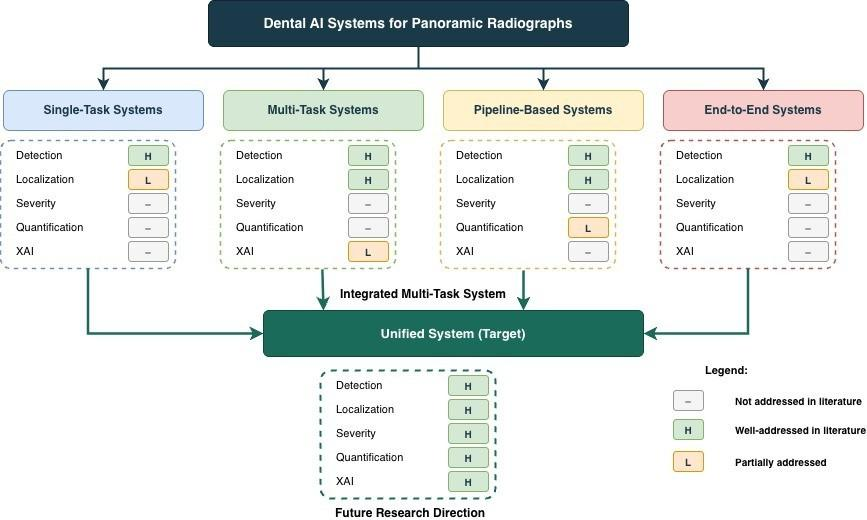
\includegraphics[width=0.8\textwidth]{figures/phase2/p2_3_02_taxonomy.jpg}
\caption[System-level taxonomy of dental AI approaches]{System-level taxonomy of dental AI approaches
for panoramic radiographs, adapted from the project's companion survey (Phase 2 report, Figure 3.2).}
\label{fig:taxonomy}
\end{figure}

\chapter{Project Requirements Specification}
\label{ch:prs}

\section{Purpose}

This chapter specifies what the OPG analysis system must do and the conditions under which it must
do it. It is written for the project guide, the examiners and any developer who maintains the code.
The requirements describe the system as delivered in Phase 3; Chapter~\ref{ch:results} reports how
well each measurable requirement is met.

\section{Product Scope}

The product is a decision-support prototype that takes one panoramic radiograph and returns a
structured, per-tooth report: which teeth are present, their FDI numbers, whether each shows caries
and how deep, and whether each overlaps an expert-style abnormality. It is meant for demonstration,
teaching and research. It is not a medical device, makes no diagnosis, and states so in every report.

\section{Product Perspective}

The system is self-contained (Figure~\ref{fig:context}). A user supplies an image through a command
line or a browser; the system loads hash-pinned model checkpoints from local storage, runs on the
CPU, and writes a JSON report and an optional overlay. It needs no network connection at inference
time, stores no patient data, and has no external dependencies beyond the Python packages it ships
with.

\begin{figure}[!htbp]
\centering
% System context. Components traced to: scripts/run_inference.py (CLI, load_models, run_pipeline),
% app.py (Streamlit), Dockerfile, models/README.md (checkpoint store), paper/paper.md Table 3 (datasets).
\begin{tikzpicture}[node distance=7mm and 10mm]
\node[stage,text width=50mm,minimum height=13mm] (sys) {OPG analysis system\\[-1pt]{\normalfont six-stage pipeline, CPU}};
\node[soft=p2grey,text width=50mm,below=4mm of sys] (store) {Model store: seven hash-pinned checkpoints (313 MB)};
\begin{scope}[on background layer]
\node[draw=p2indigo,dashed,rounded corners=4pt,line width=0.8pt,fit=(sys)(store),inner sep=6pt,
      label={[lbl,anchor=south]north:system boundary}] (bd) {};
\end{scope}
\node[io,text width=30mm,left=22mm of sys,yshift=10mm] (den) {Dentist / student\\[-1pt]{\normalfont browser}};
\node[io,text width=30mm,left=22mm of sys,yshift=-10mm] (res) {Researcher\\[-1pt]{\normalfont command line}};
\node[rept,text width=30mm,right=22mm of sys,yshift=10mm] (rep) {JSON report\\[-1pt]{\normalfont \texttt{opg-report/1.6}}};
\node[rept,text width=30mm,right=22mm of sys,yshift=-10mm] (ovl) {Overlay image};
\node[soft=p2teal,text width=44mm,below=10mm of store] (data) {Public datasets: DENTEX, Tufts, CariesXrays, Kaggle (training only, offline)};
\node[soft=p2maroon,text width=40mm,left=8mm of data] (ext) {Locked external cohorts: Ningxia, UFBA-425 (evaluation only)};
\node[soft=p2orange,text width=36mm,right=8mm of data] (dev) {Developer: tests, Docker build};
\draw[arr] (den.east) -- node[lbl,above,sloped]{upload OPG} (sys.west|-den.east);
\draw[arr] (res.east) -- node[lbl,below,sloped]{\texttt{-{}-image}} (sys.west|-res.east);
\draw[arr] (sys.east|-rep.west) -- (rep.west);
\draw[arr] (sys.east|-ovl.west) -- (ovl.west);
\draw[darr] (data.north) -- node[lbl,right]{trained checkpoints} (store.south);
\draw[darr] (ext.north) |- ($(store.south west)+(0,-2mm)$);
\draw[darr] (dev.north) |- ($(store.south east)+(0,-2mm)$);
\end{tikzpicture}

\caption[System context diagram]{System context. Users and data sources outside the boundary; the
pipeline, its model store and its outputs inside.}
\label{fig:context}
\end{figure}

\section{User Classes and Characteristics}

The system serves four classes of user, each through a different interface
(Table~\ref{tab:users}).

\begin{table}[!htbp]
\centering
\caption[User classes]{User classes and how each uses the system.}
\label{tab:users}
\small
\begin{tabularx}{\textwidth}{@{}L{3.4cm}YL{4.2cm}@{}}
\toprule
User class & Needs & Interface\\
\midrule
Dentist or dental student & Upload an OPG, see the numbered overlay and the per-tooth findings, read the limitations & Streamlit web demo\\
Researcher & Run the pipeline on many images, change checkpoints, reproduce a reported number & Command-line tool, evaluation scripts\\
Developer / maintainer & Retrain a stage, add a test, rebuild the container & Source code, test suite, Dockerfile\\
Examiner & Check that a number in the report traces to an artefact & Number-verification script, saved outputs\\
\bottomrule
\end{tabularx}
\end{table}

\section{Operating Environment}

Inference runs on a laptop or desktop CPU under Windows, macOS or Linux with Python 3.12, or inside
the provided Docker image (a CPU-only build on \texttt{python:3.12-slim}). Training was done on
cloud and laptop accelerators and is not needed to use the system.

\section{Functional Requirements}

The functional requirements, and the file that implements each, are listed in
Table~\ref{tab:fr}.

\begin{table}[!htbp]
\centering
\caption[Functional requirements]{Functional requirements and where each is implemented.}
\label{tab:fr}
\small
\begin{tabularx}{\textwidth}{@{}L{1.4cm}YL{4.0cm}@{}}
\toprule
ID & Requirement & Implemented in\\
\midrule
FR-01 & Accept one OPG as PNG or JPEG through a command-line argument or a browser upload. & \texttt{run\_inference.py}, \texttt{app.py}\\
FR-02 & Check the input and record warnings (for example an unusual bit depth) in the report rather than failing silently. & \texttt{check\_input}\\
FR-03 & Detect every tooth and return a box and a confidence per tooth, after correcting the image orientation. & Stage 1, \texttt{detect\_upright}\\
FR-04 & Assign one FDI code to each detected tooth, at most once per code, with a confidence and flags for doubtful codes. & Stage 2, Hungarian assignment\\
FR-05 & Find caries lesions on the whole image and attach each lesion to the tooth that contains most of it. & Stage 3a, lesion detector\\
FR-06 & Offer the retained per-crop caries classifier as an alternative method. & \texttt{-{}-caries-method gate}\\
FR-07 & Grade each caries-positive tooth as caries or deep caries. & Stage 3b\\
FR-08 & Flag each tooth whose expanded crop overlaps an expert-style abnormality; withhold the severity grade unless requested. & Stage 4a, \texttt{-{}-bone-severity-grade}\\
FR-09 & Mark each tooth assessable or not, with reasons, when no code was assigned or the numbering confidence is below 0.30. & Stage 5\\
FR-10 & Write one JSON report with a summary, per-tooth records, model metadata and a limitations block. & Stage 6, schema \texttt{opg-report/1.6}\\
FR-11 & Optionally write an annotated overlay image. & \texttt{-{}-overlay}, \texttt{draw\_overlay}\\
FR-12 & In the web demo, show the overlay, a per-tooth table, the limitations and the model versions, and offer the JSON report for download. & \texttt{app.py}\\
FR-13 & Let the user select any retained checkpoint to reproduce an earlier result. & CLI flags (Appendix~B)\\
FR-14 & Record provenance in every report: checkpoint paths and SHA-256 hashes, code version and device. & \texttt{runtime\_info}\\
\bottomrule
\end{tabularx}
\end{table}

\section{Non-Functional Requirements}

The non-functional requirements are listed in Table~\ref{tab:nfr}.

\begin{table}[!htbp]
\centering
\caption[Non-functional requirements]{Non-functional requirements, with the measure used to check each.}
\label{tab:nfr}
\small
\begin{tabularx}{\textwidth}{@{}L{1.7cm}L{3.0cm}YL{3.3cm}@{}}
\toprule
ID & Quality & Requirement & Measure\\
\midrule
NFR-01 & Performance & Report one OPG in a few seconds on a laptop CPU. & 1.70 s per image measured (Section~\ref{sec:res-runtime})\\
NFR-02 & Hardware independence & Need no GPU at inference. & CPU-only container\\
NFR-03 & Reproducibility & Pin every default checkpoint by hash; fix random seeds; version the report schema. & SHA-256 pins, seed 42\\
NFR-04 & Traceability & Trace every reported number to a saved artefact. & 215 numbers asserted\\
NFR-05 & Reliability & Refuse to fuse misaligned stage outputs; guard against NaN confidences. & Assertions in \texttt{build\_report}\\
NFR-06 & Usability & One command, or one browser upload; overlay colours distinguishable under red--green colour blindness. & Grey, orange and blue overlay\\
NFR-07 & Safety and honesty & State in every report that it is not clinically validated, and show the limitations beside the results. & \texttt{limitations} block\\
NFR-08 & Privacy & Run locally as a single-user demo; store no uploaded image. & No network, no storage\\
NFR-09 & Portability & Run identically from a Docker image. & Image build self-test\\
NFR-10 & Maintainability & Keep stages in separate modules with tests. & 23 test modules\\
NFR-11 & Licence compliance & Show only images whose licence allows it. & DENTEX CC BY-NC-SA 4.0\\
\bottomrule
\end{tabularx}
\end{table}

\section{Data Requirements}

Each stage needs a different label, and no single public dataset carries all of them. The datasets,
their labels and their roles are listed in Table~\ref{tab:datasets}. Two rules apply throughout:
images that are byte-identical to training images are removed from every evaluation set, and the
Ningxia cohort is never used for training or tuning.

\section{Hardware and Software Requirements}

\begin{table}[!htbp]
\centering
\caption[Hardware and software requirements]{Hardware and software requirements for using the system.
Versions: \texttt{requirements-lock.txt} and the Dockerfile.}
\label{tab:hwsw}
\small
\begin{tabularx}{\textwidth}{@{}L{4.0cm}Y@{}}
\toprule
Item & Requirement\\
\midrule
Processor & Any 64-bit laptop or desktop CPU; no GPU needed for inference\\
Operating system & Windows, macOS or Linux; or any host that runs Docker\\
Python & 3.12\\
Deep learning & PyTorch 2.2.0 (CPU build), torchvision 0.17.0, Ultralytics 8.4.127 (YOLO11)\\
Numerical & NumPy 1.26.4 (below 2, which breaks the Hungarian solver import), SciPy 1.12.0, scikit-learn 1.4.0, pandas 2.2.0\\
Imaging & OpenCV, Pillow 10.2.0, Matplotlib 3.11.1\\
Interface & Streamlit 1.64.0 for the web demo\\
Testing & pytest 7.4.4\\
Storage & The default checkpoints, about 0.3 GB, are kept in the repository\\
\bottomrule
\end{tabularx}
\end{table}

\section{Design Constraints}

\begin{itemize}
\item Each stage keeps the crop convention it was trained with: a tight $1.0\times$ crop for caries,
  $1.5\times$ by $1.5\times$ for numbering and $1.5\times$ by $2.0\times$ for the abnormality flag.
  Crossing them produces confident, wrong output with no error (Section~\ref{sec:lld-crops}).
\item The detector input size is fixed at 1,024 pixels, the confidence threshold at 0.25 and the non-maximum suppression (NMS)
  IoU at 0.50, the values the models were trained and evaluated with.
\item Field names in the report are stable across versions, so consumers do not break when a
  checkpoint changes; the meaning of each field is stated in the report itself.
\end{itemize}
% {C091}

\section{Assumptions and Dependencies}

\begin{itemize}
\item Input radiographs are adult panoramic OPGs comparable to the training corpora.
\item The public datasets remain available under their licences.
\item Reported accuracy holds only for cohorts like those evaluated; another population may have a
  different caries prior and therefore a different image-blind floor.
\end{itemize}

\section{Use Cases}

The actors and their use cases are drawn in Figure~\ref{fig:usecase} and described in
Table~\ref{tab:usecases}.

\begin{figure}[!htbp]
\centering
% Use-case diagram. Use cases traced to: app.py (upload, overlay, table, limitations, JSON download,
% model versions), scripts/run_inference.py (CLI flags), scripts/verify_paper_numbers.py, Dockerfile.
\begin{tikzpicture}[
  actor/.style={font=\sffamily\scriptsize,align=center},
  uc/.style={ellipse,draw=p2indigo,line width=0.7pt,fill=p2indigo!6,font=\sffamily\scriptsize,
             align=center,minimum width=40mm,minimum height=8.5mm,inner sep=1pt}]
\newcommand{\stick}[2]{%
  \begin{scope}[shift={#1}]
  \draw[p2grey,line width=0.8pt] (0,0.42) circle (0.13);
  \draw[p2grey,line width=0.8pt] (0,0.29) -- (0,-0.05) (-0.22,0.18) -- (0.22,0.18)
        (0,-0.05) -- (-0.17,-0.35) (0,-0.05) -- (0.17,-0.35);
  \node[actor] at (0,-0.6) {#2};
  \end{scope}}
\node[uc] (u1) at (0,3.0) {Analyse one OPG in the browser};
\node[uc] (u2) at (0,1.9) {View findings and limitations};
\node[uc] (u3) at (0,0.8) {Download the JSON report};
\node[uc] (u4) at (0,-0.3) {Run batch analysis (CLI)};
\node[uc] (u5) at (0,-1.4) {Select a retained checkpoint};
\node[uc] (u6) at (0,-2.5) {Reproduce a reported number};
\node[uc] (u7) at (5.4,-0.9) {Retrain a stage};
\node[uc] (u8) at (5.4,-2.0) {Build and run the container};
\begin{scope}[on background layer]
\node[draw=p2grey,rounded corners=4pt,line width=0.8pt,fit=(u1)(u6)(u7)(u8),inner sep=8pt,
      label={[lbl,anchor=south]north:OPG analysis system}] {};
\end{scope}
\stick{(-4.6,2.2)}{Dentist /\\student}
\stick{(-4.6,-1.0)}{Researcher}
\stick{(-4.6,-3.4)}{Examiner}
\stick{(9.0,-1.5)}{Developer}
\foreach \u in {u1,u2,u3} \draw[p2arrow,line width=0.7pt] (-4.3,2.3) -- (\u.west);
\foreach \u in {u4,u5,u6} \draw[p2arrow,line width=0.7pt] (-4.3,-0.9) -- (\u.west);
\draw[p2arrow,line width=0.7pt] (-4.3,-3.3) -- (u6.west);
\foreach \u in {u7,u8} \draw[p2arrow,line width=0.7pt] (8.7,-1.4) -- (\u.east);
\draw[darr] (u1.south) -- node[lbl,right]{\guillemotleft include\guillemotright} (u2.north);
\end{tikzpicture}

\caption[Use-case diagram]{Use-case diagram of the system.}
\label{fig:usecase}
\end{figure}

\begin{table}[!htbp]
\centering
\caption[Main use cases]{Main use cases.}
\label{tab:usecases}
\small
\begin{tabularx}{\textwidth}{@{}L{3.3cm}L{2.6cm}Y@{}}
\toprule
Use case & Actor & Flow\\
\midrule
Analyse one OPG & Dentist, student & Upload the image in the browser; the system runs all stages and shows the overlay, the per-tooth table and the limitations; the user downloads the JSON report.\\
Batch analysis & Researcher & Run the command-line tool per image (or from a script) and collect the JSON reports.\\
Reproduce a result & Researcher, examiner & Select the checkpoint named in the result's log and run the matching evaluation script; compare with the saved artefact.\\
Retrain a stage & Developer & Rebuild the stage's dataset, train with the recorded recipe and seed, register the new checkpoint's hash, rerun the tests.\\
Deploy the demo & Developer & Build the Docker image; the build fails if a dependency would break the pipeline; run it and open port 8501.\\
\bottomrule
\end{tabularx}
\end{table}

\chapter{High-Level Design}
\label{ch:hld}

\section{Design Goals}

\begin{itemize}
\item \textbf{Tooth-centric output.} The unit of every result is a numbered tooth, because that is
  how a dentist reads and records an OPG.
\item \textbf{One code path.} The command-line tool and the web demo call the same two functions
  (\texttt{load\_models}, \texttt{run\_pipeline}), so a fix or a new caveat reaches both and the demo
  cannot drift from what the evaluation measured.
\item \textbf{Modular stages.} Each stage is trained on the dataset that carries its label and can
  be replaced by another checkpoint without touching the others.
\item \textbf{Honest output.} The report carries the measured limitations of whichever checkpoints
  ran, next to the findings.
\item \textbf{Commodity hardware.} Inference on a CPU, packaged in a container.
\end{itemize}

\section{System Architecture}

The system is organised in five layers (Figure~\ref{fig:layers}). The presentation layer holds the
two entry points. The orchestration layer loads the models once, checks the input, runs the stages
in order and records provenance. The stage layer contains the six pipeline stages. The model and
artefact layer holds the hash-pinned checkpoints and the outputs. Beside them, an evaluation layer of
scripts and tests reproduces every number reported in Chapter~\ref{ch:results}.

\begin{figure}[!htbp]
\centering
% Layered architecture. Components traced to: app.py, scripts/run_inference.py (main, load_models,
% run_pipeline, runtime_info, check_input, build_report, draw_overlay), src/*.py, models/README.md,
% scripts/eval/, scripts/verify_paper_numbers.py, tests/.
\begin{tikzpicture}[
  lay/.style={rectangle,rounded corners=3pt,draw=#1,line width=0.8pt,fill=#1!6,minimum width=128mm,
              minimum height=14mm,inner sep=3pt},
  lname/.style={font=\sffamily\scriptsize\bfseries,text=#1,anchor=west},
  comp/.style={box,fill=#1,text width=27mm,minimum height=8mm,font=\sffamily\tiny\bfseries}]
% layers
\node[lay=p2grey]   (L1) at (0,0)     {};
\node[lay=p2indigo] (L2) at (0,-1.75) {};
\node[lay=p2teal,minimum height=17mm] (L3) at (0,-3.85) {};
\node[lay=p2green]  (L4) at (0,-5.75) {};
\node[lname=p2grey]   at ($(L1.north west)+(1mm,-2mm)$) {Presentation};
\node[lname=p2indigo] at ($(L2.north west)+(1mm,-2mm)$) {Orchestration};
\node[lname=p2teal]   at ($(L3.north west)+(1mm,-2mm)$) {Stages};
\node[lname=p2green]  at ($(L4.north west)+(1mm,-2mm)$) {Models and artefacts};
% presentation
\node[comp=p2grey] at (-2.2,-0.15) {CLI\\\texttt{run\_inference.py main}};
\node[comp=p2grey] at (2.2,-0.15)  {Web demo\\\texttt{app.py} (Streamlit)};
% orchestration
\node[comp=p2indigo] at (-4.4,-1.9) {\texttt{load\_models}\\hash-pinned loads};
\node[comp=p2indigo] at (-1.45,-1.9) {\texttt{check\_input}\\input warnings};
\node[comp=p2indigo] at (1.5,-1.9)  {\texttt{run\_pipeline}\\Stages 1--6};
\node[comp=p2indigo] at (4.45,-1.9) {\texttt{runtime\_info}\\provenance};
% stages (two rows)
\node[comp=p2teal,text width=19mm] at (-5.05,-4.0) {1 Detect\\YOLOv11l};
\node[comp=p2teal,text width=19mm] at (-2.95,-4.0) {2 Number\\ResNet18 + Hungarian};
\node[comp=p2teal,text width=19mm] at (-0.85,-4.0) {3a Caries\\lesion detector};
\node[comp=p2teal,text width=19mm] at (1.25,-4.0) {3b Severity\\ResNet18};
\node[comp=p2maroon,text width=19mm] at (3.35,-4.0) {4a Abnormality\\ResNet18};
\node[comp=p2orange,text width=19mm] at (5.45,-4.0) {5--6 Fuse +\\report, overlay};
% models
\node[comp=p2green,text width=36mm] at (-3.6,-5.9) {Checkpoints \texttt{models/<NN>\_*}\\SHA-256 pinned};
\node[comp=p2green,text width=36mm] at (0.6,-5.9)  {JSON report\\\texttt{opg-report/1.6}};
\node[comp=p2green,text width=30mm] at (4.6,-5.9)  {Overlay image};
% evaluation layer at the side
\node[rectangle,rounded corners=3pt,draw=p2orange,line width=0.8pt,fill=p2orange!8,text width=24mm,
      minimum height=73mm,font=\sffamily\tiny,align=center] (ev) at (8.25,-2.9)
      {\textbf{\scriptsize Evaluation}\\[2mm]\texttt{scripts/eval/}\\40 scripts\\[2mm]\texttt{verify\_paper\_numbers}\\215 numbers\\[2mm]\texttt{tests/}\\23 modules};
\draw[arr] (L1.south) -- (L2.north);
\draw[arr] (L2.south) -- (L3.north);
\draw[darr] (L3.south) -- (L4.north);
\draw[darr] (ev.west|-L3) -- (L3.east);
\end{tikzpicture}

\caption[Layered system architecture]{Layered architecture. Arrows show calls; dashed arrows show
data read from or written to storage.}
\label{fig:layers}
\end{figure}

\section{Data Flow}

At level 0 the system is one process: an OPG goes in, a report and an overlay come out. At level 1
(Figure~\ref{fig:dfd}) the six stages exchange well-defined intermediate data: boxes and detection
confidences, FDI assignments, lesion boxes and caries findings, abnormality flags, and fused
per-tooth records.

\begin{figure}[!htbp]
\centering
% Data-flow diagram, levels 0 and 1. Flows traced to scripts/run_inference.py run_pipeline() and
% build_report(): boxes+confs -> fdi_assign -> caries -> bone -> teeth records -> report.
\begin{tikzpicture}[
  proc/.style={circle,draw=none,fill=#1,text=white,font=\sffamily\tiny\bfseries,align=center,
               minimum size=15mm,inner sep=1pt},
  ext/.style={rectangle,draw=p2grey,line width=0.8pt,fill=lgrey,font=\sffamily\scriptsize,align=center,
              minimum width=20mm,minimum height=8mm},
  store/.style={rectangle,draw=p2grey,line width=0.6pt,font=\sffamily\tiny,align=left,
                minimum width=30mm,minimum height=6mm,path picture={\draw[p2grey,line width=0.6pt]
                ([xshift=5mm]path picture bounding box.north west) -- ([xshift=5mm]path picture bounding box.south west);}},
  fl/.style={font=\sffamily\tiny,text=p2grey,align=center}]
% level 0
\node[ext] (u0) at (-5.4,0) {User};
\node[proc=p2indigo,minimum size=17mm] (p0) at (0,0) {0\\OPG analysis\\system};
\node[ext] (o0) at (5.4,0) {Report and\\overlay};
\draw[arr] (u0) -- node[fl,above]{OPG image} (p0);
\draw[arr] (p0) -- node[fl,above]{per-tooth JSON, JPG} (o0);
\node[lbl] at (0,1.25) {\textbf{Level 0}};
% level 1
\node[lbl] at (-6.0,-1.55) {\textbf{Level 1}};
\node[ext] (u1) at (-6.6,-3.3) {User};
\node[proc=p2indigo] (s1) at (-4.4,-3.3) {1.0\\Detect\\teeth};
\node[proc=p2indigo] (s2) at (-1.9,-3.3) {2.0\\Number\\(FDI)};
\node[proc=p2teal]   (s3) at (0.6,-3.3)  {3.0\\Find\\caries};
\node[proc=p2maroon] (s4) at (3.1,-3.3)  {4.0\\Flag\\abnorm.};
\node[proc=p2orange] (s5) at (5.6,-3.3)  {5.0\\Fuse +\\assess};
\node[proc=p2green]  (s6) at (5.6,-5.8)  {6.0\\Write\\report};
\node[store] (d1) at (-1.9,-5.8) {D1\quad Model checkpoints};
\node[store] (d2) at (2.0,-5.8) {D2\quad Report, overlay};
\draw[arr] (u1) -- node[fl,above]{image} (s1);
\draw[arr] (s1) -- node[fl,above]{boxes,\\conf.} (s2);
\draw[arr] (s2) -- node[fl,above]{codes,\\conf.} (s3);
\draw[arr] (s3) -- node[fl,above]{caries\\finding} (s4);
\draw[arr] (s4) -- node[fl,above]{flag} (s5);
\draw[arr] (s5) -- node[fl,right]{tooth\\records} (s6);
\draw[arr] (s6) -- (d2);
\foreach \s in {s1,s2,s3,s4} \draw[darr] (d1.north) -- (\s.south);
\draw[darr] (s1.north) to[bend left=22] node[fl,above]{boxes reused by every stage} (s4.north);
\end{tikzpicture}

\caption[Data-flow diagram, levels 0 and 1]{Data-flow diagram. Top: level 0. Bottom: level 1, with
the model store (D1) read by every stage and the report store (D2) written by Stage~6.}
\label{fig:dfd}
\end{figure}

\section{Deployment Architecture}

The demo is distributed as a Docker image (Figure~\ref{fig:deploy}). The image starts from a slim
Python 3.12 base, installs a CPU-only PyTorch build and the pinned packages, and copies the
application, the scripts, the source modules and the model checkpoints. During the build a self-test
imports every dependency and runs the Hungarian solver once, so an incompatible package fails the
build instead of the first upload. The container serves Streamlit on port 8501 and reports its health
on Streamlit's health endpoint.

\begin{figure}[!htbp]
\centering
% Deployment. Traced to Dockerfile (FROM python:3.12.12-slim; COPY app.py scripts/ src/ models/;
% build self-test; EXPOSE 8501; HEALTHCHECK /_stcore/health; CMD streamlit run app.py).
\begin{tikzpicture}[
  host/.style={rectangle,rounded corners=4pt,draw=p2grey,line width=0.9pt,fill=lgrey,inner sep=6pt},
  ctr/.style={rectangle,rounded corners=4pt,draw=p2indigo,line width=0.9pt,fill=p2indigo!5,inner sep=6pt},
  cmp/.style={box,fill=#1,text width=34mm,minimum height=8mm,font=\sffamily\tiny\bfseries}]
\node[cmp=p2indigo] (st) at (0,0) {Streamlit server\\\texttt{app.py}, port 8501};
\node[cmp=p2teal]   (pl) at (0,-1.25) {Pipeline\\\texttt{load\_models}, \texttt{run\_pipeline}};
\node[cmp=p2green]  (md) at (0,-2.5) {Model checkpoints\\\texttt{models/} (copied at build)};
\node[cmp=p2grey]   (py) at (0,-3.75) {Python 3.12 slim + CPU PyTorch\\pinned packages};
\node[soft=p2orange,text width=34mm] (hc) at (4.3,0) {Health check every 30 s\\\texttt{/\_stcore/health}};
\node[soft=p2orange,text width=34mm] (bt) at (4.3,-3.75) {Build self-test: imports,\\Hungarian solver, numpy below 2};
\begin{scope}[on background layer]
\node[ctr,fit=(st)(py)(hc)(bt),label={[lbl,anchor=south]north:Docker container}] (c) {};
\end{scope}
\node[cmp=p2grey,text width=26mm] (br) at (-5.0,0) {Browser\\\texttt{localhost:8501}};
\node[cmp=p2grey,text width=26mm] (cli) at (-5.0,-2.0) {Host CLI\\\texttt{run\_inference.py}};
\draw[arr] (br) -- node[lbl,above]{upload} (st);
\draw[arr] (st) -- (pl); \draw[darr] (md) -- (pl); \draw[p2arrow,line width=0.6pt] (py) -- (md);
\draw[arr] (cli.east) -- node[lbl,below,sloped]{same functions} ($(pl.west)+(-0.3,0)$) -- (pl.west);
\draw[p2arrow,line width=0.6pt,dashed] (hc.west) -- (st.east);
\end{tikzpicture}

\caption[Deployment architecture]{Deployment. The same pipeline runs on the host through the command
line or inside the container behind the Streamlit server.}
\label{fig:deploy}
\end{figure}

\section{From the Phase 2 Target to the As-Built Pipeline}

The Phase 2 report drew the target pipeline reproduced in Figure~\ref{fig:p2target}: YOLO tooth
detection, sorting into FDI order, a per-tooth loop with a tight crop for caries and an expanded crop
for bone loss, a filter that kept only positive teeth, and a final report. Phase 3 built that design
with four deliberate changes (Table~\ref{tab:target-vs-built}); the as-built pipeline is shown in
Figure~\ref{fig:arch} of Chapter~\ref{ch:system}. % {C092}

\begin{figure}[!htbp]
\centering
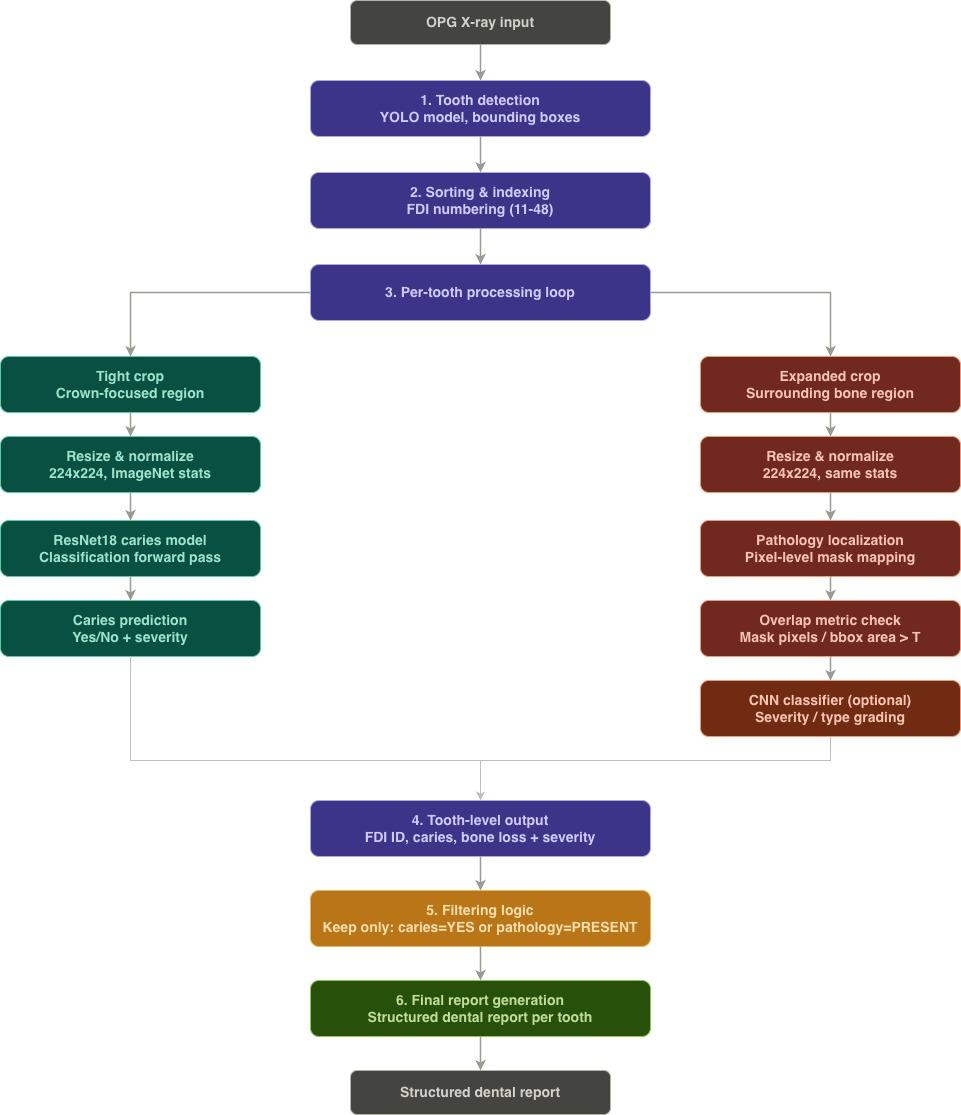
\includegraphics[width=0.62\textwidth]{figures/phase2/p2_3_01_target_pipeline.jpg}
\caption[Phase 2 target architecture]{The target end-to-end architecture drawn in the Phase 2 report
(Figure 3.1 there).}
\label{fig:p2target}
\end{figure}

\begin{table}[!htbp]
\centering
\caption[Phase 2 target design against the as-built design]{Phase 2 target design against the
as-built design, with the reason for each change.}
\label{tab:target-vs-built}
\small
\begin{tabularx}{\textwidth}{@{}L{3.0cm}L{3.6cm}L{3.8cm}Y@{}}
\toprule
Element & Phase 2 target & Phase 3 as built & Reason\\
\midrule
Numbering & Sort boxes into FDI order & Learned ResNet18 head plus Hungarian one-to-one assignment & Sorting fails when teeth are missing or tilted; a learned head with a one-to-one constraint cannot emit duplicate codes\\
Caries & Tight-crop classifier & Whole-image lesion detector, crop classifier retained & Five repairs of the classifier failed; the detector met a pre-registered rule\\
Bone loss & Overlap-labelled classifier with severity & Abnormality flag, severity withheld & The label marks expert abnormalities, not bone loss; the severity head did not beat a position prior\\
Filtering & Keep only positive teeth & Report every tooth, with an assessable flag & A missing tooth must be distinguishable from a healthy one\\
\bottomrule
\end{tabularx}
\end{table}

\section{Design Rationale}

The tooth-centric formulation was chosen over an image-level classifier because the deliverable is a
tooth-wise report, not one disease flag for the whole OPG. A modular pipeline is also the practical
answer to the available data: DENTEX provides tooth-level caries labels, Tufts is richer for
abnormality masks after region-to-tooth mapping, CariesXrays provides lesion boxes, and no single
dataset contains every label in one consistent format. A monolithic multi-task model would add
supervision mismatch without a clear advantage.

ResNet18 is the common backbone of the four classifier heads because it is light, well understood
and stable under transfer learning on small dental datasets; larger backbones were avoided because
the extra capacity raises overfitting risk without a demonstrated benefit. The two detectors are
YOLOv11l~\cite{jocher2024yolo11}, which balances accuracy and speed on a large panoramic image.

The modular design moves responsibility to integration: numbering, report assembly, consistency
checks and confidence handling must make independently trained models behave as one system. Phase 3
therefore added four mechanisms:
\begin{itemize}
\item a one-to-one assignment that forbids duplicate FDI codes;
\item an assessability rule that marks a tooth whose number is uncertain;
\item a check that refuses to fuse stage outputs of different lengths;
\item a limitations block in the report, keyed to the hash of each checkpoint that ran.
\end{itemize}

The caries stage changed form during Phase 3. The per-crop classifier of Phase 2 sees one tight crop
and answers yes or no, a task in which a strong positional prior can earn much of the score; five
direct repairs of it, each against a same-day control, gave no gain that separated from zero
(Section~\ref{sec:res-rq2}). The task was therefore changed to locating lesions on the whole image,
under an acceptance rule committed before any candidate was trained, and the classifier was kept as
a selectable alternative. % {C071}

\chapter{Low-Level Design}
\label{ch:lld}

\section{Module Decomposition}

The code is split into reusable modules under \texttt{src/}, an integration script, a web wrapper and
evaluation scripts (Table~\ref{tab:modules}, Figure~\ref{fig:modules}). Each module owns one
convention, such as a crop geometry or a coordinate frame, and defines its constants once, because a
silent mismatch between training and inference preprocessing degrades accuracy without raising any
error.

\begin{table}[!htbp]
\centering
\caption[Module decomposition]{Module decomposition (repository on 2 November 2026).}
\label{tab:modules}
\small
\begin{tabularx}{\textwidth}{@{}L{4.4cm}YL{4.5cm}@{}}
\toprule
Module & Responsibility & Key functions\\
\midrule
\nolinkurl{scripts/run_inference.py} & Integration: Stages 5--6, model loading, provenance, CLI & \texttt{load\_models}, \texttt{run\_pipeline}, \texttt{build\_report}, \texttt{draw\_overlay}\\
\nolinkurl{app.py} & Streamlit web demo, a thin wrapper over the same functions & \texttt{get\_models}, page layout\\
\nolinkurl{src/orientation.py} & Rotates the image into the detector's training frame and maps boxes back & \texttt{detect\_upright}, \texttt{unrot\_boxes}\\
\nolinkurl{src/fdi_head_inference.py} & Stage 2: crops, box features, joint scores, one-to-one assignment & \texttt{assign\_fdi\_head}, \texttt{head\_joint\_scores}\\
\nolinkurl{src/classifiers.py} & Stages 3--4: crop batches, caries gate, lesion detector, severity, abnormality flag & \nolinkurl{run_caries_lesion_detector}, \texttt{run\_caries}, \texttt{run\_bone\_loss}\\
\nolinkurl{src/crop_generator.py} & Expanded boxes, jitter, mask-aware crops (Phase 2) & \texttt{compute\_expanded\_bbox}\\
\nolinkurl{src/label_assigner.py} & Overlap-ratio labels for the abnormality flag (Phase 2) & \texttt{compute\_overlap\_ratio}\\
\nolinkurl{src/data_loader.py} & Tufts annotation parsing and joins (Phase 2) & \texttt{join\_all\_sources}\\
\nolinkurl{src/fdi_assignment.py} & Rule-based arch ordering, kept for comparison & \texttt{assign\_fdi}\\
\nolinkurl{src/fdi_structural_repair.py} & Optional sequence repair after assignment (an ablation, off by default) & \texttt{structural\_repair}\\
\nolinkurl{src/utils/fdi_converter.py} & Universal--FDI conversion and quadrant mirroring & \texttt{universal\_to\_fdi}\\
\bottomrule
\end{tabularx}
\end{table}

\begin{figure}[!htbp]
\centering
% Module dependencies. Traced to the import statements of app.py, scripts/run_inference.py and src/*.py.
\begin{tikzpicture}[
  mod/.style={rectangle,rounded corners=2.5pt,draw=#1,line width=0.8pt,fill=#1!7,font=\sffamily\tiny,
              align=left,text width=40mm,inner sep=3pt},
  mt/.style={font=\sffamily\scriptsize\bfseries,text=#1}]
\node[mod=p2grey] (app) at (-3.2,0) {\textbf{app.py}\\get\_models()\\page: upload, overlay, table, limitations};
\node[mod=p2grey] (cli) at (3.2,0) {\textbf{scripts/run\_inference.py}\\main(), load\_models(), run\_pipeline()\\build\_report(), draw\_overlay(), runtime\_info()};
\node[mod=p2indigo] (ori) at (-5.2,-2.3) {\textbf{src/orientation.py}\\detect\_upright()\\rot\_boxes(), unrot\_boxes()};
\node[mod=p2indigo] (fdi) at (0,-2.3) {\textbf{src/fdi\_head\_inference.py}\\assign\_fdi\_head()\\head\_joint\_scores() (32 codes)};
\node[mod=p2teal] (cls) at (5.2,-2.3) {\textbf{src/classifiers.py}\\run\_caries\_lesion\_detector()\\run\_caries(), run\_bone\_loss()\\lesion\_preds\_to\_tooth\_idx()};
\node[mod=p2maroon] (crop) at (2.6,-4.6) {\textbf{src/crop\_generator.py}\\compute\_expanded\_bbox()};
\node[mod=p2orange] (rep) at (-2.6,-4.6) {\textbf{src/fdi\_structural\_repair.py}\\structural\_repair() (optional)};
\node[mod=p2green] (ext) at (0,-6.5) {\textbf{External}\\Ultralytics YOLO11, PyTorch, OpenCV, SciPy (linear\_sum\_assignment)};
\draw[arr] (app) -- node[lbl,above]{imports} (cli);
\draw[arr] (cli) -- (ori); \draw[arr] (cli) -- (fdi); \draw[arr] (cli) -- (cls);
\draw[arr] (fdi) -- (crop); \draw[arr] (cls) -- (crop); \draw[darr] (fdi) -- (rep);
\draw[darr] (ori.south) |- (ext.west); \draw[darr] (cls.south) |- (ext.east);
\end{tikzpicture}

\caption[Module dependency diagram]{Module dependency diagram. Arrows point from a caller to the
module it uses.}
\label{fig:modules}
\end{figure}

\section{Stage Interfaces}

Every stage consumes the tooth boxes of Stage~1 and returns exactly one entry per box, in box order,
so Stage~5 can fuse the outputs by position (Table~\ref{tab:interfaces}).

\begin{table}[!htbp]
\centering
\caption[Stage interfaces]{Stage interfaces: input, crop convention, model and output.}
\label{tab:interfaces}
\small
\begin{tabularx}{\textwidth}{@{}L{1.6cm}L{3.0cm}L{2.5cm}L{3.0cm}Y@{}}
\toprule
Stage & Input & Crop & Model & Output per tooth\\
\midrule
1 & OPG, rotated 90\textdegree\ counter-clockwise & whole image, 1,024 px & YOLOv11l, conf.\ 0.25, NMS IoU 0.50 & box, detection confidence\\
2 & boxes & $1.5\times1.5$, 224 px, RGB & ResNet18 + 4 box features & FDI code, confidence, flags\\
3a & OPG, boxes & whole image & YOLOv11l lesion detector, conf.\ 0.25 & caries finding\\
3b & caries-positive teeth & $1.0\times1.0$ (tight), 224 px & ResNet18 & caries or deep caries\\
4a & boxes & $1.5\times2.0$, 224 px & ResNet18 & normal or flagged, confidence\\
4b & flagged teeth & $1.5\times2.0$ & ResNet18 & severity (withheld by default)\\
5 & all of the above & --- & rules & assessable flag and reasons\\
6 & tooth records, metadata & --- & --- & JSON report, overlay\\
\bottomrule
\end{tabularx}
\end{table}

\subsection{Crop Conventions}
\label{sec:lld-crops}

The three crop geometries come from three training pipelines (Figure~\ref{fig:crops}). Caries is
judged on a tight crop of the crown. Numbering sees the tooth and some of its neighbours, so that
position along the arch is visible. The abnormality flag sees the root and surrounding bone, so its
crop is widened by 1.5 and lengthened by 2.0 times the box. Crossing the conventions produces
confident, plausible and wrong output, so each constant is defined once in the module that owns it.

\begin{figure}[!htbp]
\centering
% Crop conventions. Traced to src/classifiers.py (CARIES_EXPAND (1.0,1.0), BONE_LOSS_EXPAND (1.5,2.0))
% and src/fdi_head_inference.py (EXPAND 1.5). Schematic, not to scale of any real tooth.
\begin{tikzpicture}[scale=0.9]
\def\w{1.2}\def\h{2.0}
\foreach \x/\name/\fw/\fh/\col/\lab in {0/a/1.0/1.0/p2teal/{Caries: $1.0\times1.0$ (tight)},
                                        4.2/b/1.5/1.5/p2indigo/{Numbering: $1.5\times1.5$},
                                        8.6/c/1.5/2.0/p2maroon/{Abnormality: $1.5\times2.0$}} {
  \begin{scope}[shift={(\x,0)}]
  % tooth silhouette
  \fill[lgrey] (-0.45,0.9) .. controls (-0.55,0.3) and (-0.35,-0.2) .. (-0.25,-0.95)
               -- (-0.05,-0.95) -- (0,-0.3) -- (0.05,-0.95) -- (0.25,-0.95)
               .. controls (0.35,-0.2) and (0.55,0.3) .. (0.45,0.9) -- cycle;
  \draw[p2grey,line width=0.6pt] (-0.45,0.9) .. controls (-0.55,0.3) and (-0.35,-0.2) .. (-0.25,-0.95)
               -- (-0.05,-0.95) -- (0,-0.3) -- (0.05,-0.95) -- (0.25,-0.95)
               .. controls (0.35,-0.2) and (0.55,0.3) .. (0.45,0.9) -- cycle;
  \draw[black,line width=0.8pt] (-\w/2,-\h/2) rectangle (\w/2,\h/2);
  \draw[\col,line width=1.2pt,dashed] (-\w*\fw/2,-\h*\fh/2) rectangle (\w*\fw/2,\h*\fh/2);
  \node[font=\sffamily\scriptsize,text=\col,align=center] at (0,-\h*\fh/2-0.4) {\lab};
  \end{scope}}
\node[font=\sffamily\tiny,text=p2grey] at (11.4,1.0) {solid: detected box};
\node[font=\sffamily\tiny,text=p2grey] at (11.4,0.6) {dashed: crop};
\end{tikzpicture}

\caption[Crop conventions of the three classifier heads]{Crop conventions. The detected tooth box
(solid) and the three crops cut from it.}
\label{fig:crops}
\end{figure}

\section{Control Flow}

Figure~\ref{fig:sequence} shows one call of \texttt{run\_pipeline}, the function both entry points
use. Models are loaded once per process and reused. \texttt{run\_pipeline} itself writes nothing to
disk: the command-line tool writes the report (and the overlay, if asked), and the web demo draws the
overlay in memory and stores nothing.

\begin{figure}[!htbp]
\centering
% Sequence of one inference call. Traced to scripts/run_inference.py run_pipeline() (order of calls:
% check_input, detect_upright, assign_fdi_head, run_caries_lesion_detector, run_bone_loss, build_report)
% and app.py (load_models once via st.cache_resource, draw_overlay in memory).
\begin{tikzpicture}[
  ll/.style={box,fill=#1,text width=19mm,minimum height=7mm,font=\sffamily\tiny\bfseries},
  msg/.style={-{Stealth[length=2mm]},draw=p2grey,line width=0.6pt},
  ret/.style={-{Stealth[length=2mm]},draw=p2arrow,line width=0.6pt,dashed},
  mt/.style={font=\sffamily\tiny,fill=white,inner sep=1pt}]
\foreach \i/\n/\c/\t in {0/u/p2grey/User, 1/a/p2grey/{app.py / CLI}, 2/r/p2indigo/run\_pipeline,
                         3/d/p2indigo/Stage 1, 4/f/p2indigo/Stage 2, 5/c/p2teal/Stage 3, 6/b/p2maroon/Stage 4,
                         7/p/p2orange/build\_report} {
  \node[ll=\c] (\n) at (\i*2.05,0) {\t};
  \draw[p2arrow,line width=0.5pt,dotted] (\n.south) -- ++(0,-8.9);
}
\def\y#1{-#1*0.62-0.7}
\draw[msg] (u.south |- 0,{\y{0}}) -- node[mt,above]{OPG} (a.south |- 0,{\y{0}});
\draw[msg] (a.south |- 0,{\y{1}}) -- node[mt,above]{image, models} (r.south |- 0,{\y{1}});
\draw[msg] (r.south |- 0,{\y{2}}) -- node[mt,above]{rotate, detect} (d.south |- 0,{\y{2}});
\draw[ret] (d.south |- 0,{\y{3}}) -- node[mt,above]{boxes} (r.south |- 0,{\y{3}});
\draw[msg] (r.south |- 0,{\y{4}}) -- node[mt,above]{boxes} (f.south |- 0,{\y{4}});
\draw[ret] (f.south |- 0,{\y{5}}) -- node[mt,above]{codes} (r.south |- 0,{\y{5}});
\draw[msg] (r.south |- 0,{\y{6}}) -- node[mt,above]{image, boxes} (c.south |- 0,{\y{6}});
\draw[ret] (c.south |- 0,{\y{7}}) -- node[mt,above]{caries} (r.south |- 0,{\y{7}});
\draw[msg] (r.south |- 0,{\y{8}}) -- node[mt,above]{boxes} (b.south |- 0,{\y{8}});
\draw[ret] (b.south |- 0,{\y{9}}) -- node[mt,above]{flags} (r.south |- 0,{\y{9}});
\draw[msg] (r.south |- 0,{\y{10}}) -- node[mt,above]{all outputs} (p.south |- 0,{\y{10}});
\draw[ret] (p.south |- 0,{\y{11}}) -- node[mt,above]{report} (r.south |- 0,{\y{11}});
\draw[ret] (r.south |- 0,{\y{12}}) -- node[mt,above]{report} (a.south |- 0,{\y{12}});
\draw[ret] (a.south |- 0,{\y{13}}) -- node[mt,above]{overlay, table, JSON} (u.south |- 0,{\y{13}});
\end{tikzpicture}

\caption[Sequence diagram of one inference call]{Sequence diagram of one inference call.}
\label{fig:sequence}
\end{figure}

\section{Report Data Structure}
\label{sec:lld-report}

The report is one JSON object with schema version \texttt{opg-report/1.6} and seven top-level fields
(Table~\ref{tab:schema}). Field names have stayed stable while checkpoints changed, so consumers do
not break; what each field means for the checkpoint that ran is written into the report's
\texttt{limitations} block.

\begin{table}[!htbp]
\centering
\caption[Report schema]{Top-level fields of the report (\texttt{opg-report/1.6}).}
\label{tab:schema}
\small
\begin{tabularx}{\textwidth}{@{}L{3.2cm}Y@{}}
\toprule
Field & Content\\
\midrule
\texttt{schema\_version} & \texttt{opg-report/1.6}\\
\texttt{generated} & ISO timestamp\\
\texttt{image} & path, width, height, input warnings\\
\texttt{summary} & teeth detected, teeth assessable, distinct and duplicate FDI codes, caries-positive and flagged counts\\
\texttt{teeth} & one record per detected tooth, sorted by FDI code (below)\\
\texttt{models} & for each stage: checkpoint path, SHA-256, version tag and settings; runtime versions, git commit and device\\
\texttt{limitations} & detector recall and end-to-end numbering accuracy of the detector that ran and where they hold, caveats for the caries method, the meaning and validation of the Stage-4 label, and \texttt{not\_clinically\_validated: true}\\
\bottomrule
\end{tabularx}
\end{table}

A tooth record holds the box, the detection confidence, the FDI code with its quadrant, position,
confidence and flags, the caries finding, the Stage-4 finding, and the assessability decision.
Listing~\ref{lst:record} is the record for tooth 36 of the radiograph walked through in
Figure~\ref{fig:walkthrough}.

\begin{lstlisting}[caption={Report record for tooth 36 of DENTEX \texttt{test\_0} (abridged from the saved report).},label=lst:record,language={}]
{"detection_index": 0, "bbox_xyxy": [1726.8, 845.0, 1913.9, 1150.0],
 "detection_confidence": 0.8389,
 "fdi": 36, "quadrant": 3, "position": 6, "fdi_confidence": 0.9999, "fdi_flags": [],
 "caries": {"finding": "deep_caries", "gate_confidence": 0.8892,
            "severity": "deep_caries", "severity_confidence": 0.9579,
            "flags": ["lesion_detector_v1.0", "gate_confidence_is_detection_not_softmax"]},
 "bone_loss": {"finding": "normal", "confidence": 0.7853, "severity": null},
 "assessable": true, "not_assessable_reasons": []}
\end{lstlisting}

\section{Assessability and Error Handling}

\begin{itemize}
\item \textbf{Assessability.} A tooth is not assessable if no FDI code was assigned or its numbering
  confidence is below 0.30. The comparison is written as ``not $\ge 0.30$'', so a NaN confidence
  also fails. The reasons are listed in the record.
\item \textbf{Alignment check.} Before fusion, \texttt{build\_report} checks that every stage returned
  one entry per box and raises an error otherwise, instead of attaching one tooth's findings to
  another.
\item \textbf{Input checks.} \texttt{check\_input} records warnings such as an unusual bit depth in
  the report.
\item \textbf{Non-finite scores.} The numbering head raises an error on a non-finite score rather
  than assigning codes from it.
\item \textbf{Empty images.} If no tooth is detected, an empty report is written, not an error.
\end{itemize}

\section{Configuration and Model Registry}

Every default checkpoint is pinned by its SHA-256 hash, and the hash is written into each report
(Table~\ref{tab:registry}). A previous default stays selectable from the command line, so every
number published before a change can be reproduced.

\begin{table}[!htbp]
\centering
\caption[Default checkpoints]{Default checkpoints, with the first eight hexadecimal digits of each
SHA-256 hash as written in the reports.}
\label{tab:registry}
\small
\begin{tabularx}{\textwidth}{@{}L{2.8cm}YL{2.0cm}@{}}
\toprule
Stage & Checkpoint & SHA-256\\
\midrule
1 Detector & \nolinkurl{models/15_detector_multicorpus_leverA/arm3c_best.pt} & \texttt{5d301f13}\\
2 Numbering & \nolinkurl{models/10_fdi_head_dentex_tufts_v2/enumeration_head_best.pth} & \texttt{6c675fa0}\\
3a Lesion detector & \nolinkurl{models/16_lever_b_pooled/.../weights/best.pt} & \texttt{029018db}\\
3b Severity & \nolinkurl{models/07_caries_cascade/phase2_final_bundle.pth} & \texttt{aa0a8a7e}\\
4a Abnormality flag & \nolinkurl{models/18_bone_loss_radiograph_split/seed42_best.pth} & \texttt{e4bc8744}\\
4b Severity (withheld) & \nolinkurl{models/04_bone_loss_severity_notebook_models/..._best.pth} & \texttt{fa93a520}\\
\bottomrule
\end{tabularx}
\end{table}

\section{Test Design}

The test suite has 23 modules under \texttt{tests/}. They cover:
\begin{itemize}
\item the FDI converter and its lower-arch regression;
\item crop parity between training and inference;
\item orientation round trips;
\item assignment and structural repair;
\item the dataset loaders;
\item the report;
\item an end-to-end pipeline run on a fixed image;
\item a set of invariants checked against the saved artefacts.
\end{itemize}
% {C096}
Tests that need the raw Tufts radiographs skip when the data are absent. Section~\ref{sec:impl-verify}
reports the verification results.

\chapter{System Design (Detailed)}
\label{ch:system}

\section{Overview}

The pipeline maps an OPG to a per-tooth record in six stages. Figure~\ref{fig:flow} draws it in the
style of the Phase 2 target pipeline. Figure~\ref{fig:arch} gives the as-shipped version with each
default checkpoint and its learnable parameter count. Figure~\ref{fig:walkthrough} follows one
held-out radiograph through every stage.

\begin{figure}[!htbp]
\centering
% As-built pipeline in the Phase 2 Figure 3.1 style and palette. Components traced to
% scripts/run_inference.py (docstring stage list, DEF_* checkpoints, CARIES_LESION_CONF 0.25,
% ASSESSABILITY_MIN_FDI_CONFIDENCE 0.30) and src/classifiers.py (crop conventions).
\begin{tikzpicture}[node distance=4.2mm]
\node[io] (in) {OPG X-ray input\\[-1pt]{\normalfont PNG or JPEG, any size}};
\node[stage,below=of in] (s1) {1. Tooth detection\\[-1pt]{\normalfont YOLOv11l, multi-corpus, conf.\ 0.25}};
\node[stage,below=of s1] (s2) {2. FDI numbering\\[-1pt]{\normalfont ResNet18 + box features, Hungarian one-to-one}};
\node[stage,below=of s2] (s3) {3. Per-tooth processing};
\node[cari,below left=7mm and 6mm of s3] (c1) {3a. Lesion detector\\[-1pt]{\normalfont whole image, conf.\ 0.25}};
\node[cari,below=of c1] (c2) {Lesion $\rightarrow$ tooth\\[-1pt]{\normalfont argmax containment}};
\node[cari,below=of c2] (c3) {3b. Severity\\[-1pt]{\normalfont tight crop, ResNet18}};
\node[cari,below=of c3] (c4) {Caries finding\\[-1pt]{\normalfont none / caries / deep}};
\node[bone,below right=7mm and 6mm of s3] (b1) {Expanded crop\\[-1pt]{\normalfont 1.5$\times$ width, 2.0$\times$ height}};
\node[bone,below=of b1] (b2) {4a. Abnormality flag\\[-1pt]{\normalfont ResNet18, radiograph split}};
\node[bone,below=of b2] (b3) {4b. Severity\\[-1pt]{\normalfont withheld by default}};
\node[bone,below=of b3] (b4) {Abnormality finding\\[-1pt]{\normalfont normal / flagged}};
\coordinate (mid) at ($(c4.south)!0.5!(b4.south)+(0,-6mm)$);
\node[stage,below=12mm of mid] (s5) {5. Fusion and assessability\\[-1pt]{\normalfont FDI confidence $\geq$ 0.30, alignment check}};
\node[rept,below=of s5] (s6) {6. Report generation\\[-1pt]{\normalfont JSON \texttt{opg-report/1.6} + overlay}};
\node[io,below=of s6] (out) {Structured per-tooth report\\[-1pt]{\normalfont with limitations and provenance}};
\draw[arr] (in) -- (s1); \draw[arr] (s1) -- (s2); \draw[arr] (s2) -- (s3);
\draw[arr] (s3.south) -- ++(0,-3mm) -| (c1.north);
\draw[arr] (s3.south) -- ++(0,-3mm) -| (b1.north);
\draw[arr] (c1) -- (c2); \draw[arr] (c2) -- (c3); \draw[arr] (c3) -- (c4);
\draw[arr] (b1) -- (b2); \draw[arr] (b2) -- (b3); \draw[arr] (b3) -- (b4);
\draw[arr] (c4.south) |- ($(s5.north)+(0,5mm)$) -- (s5.north);
\draw[arr] (b4.south) |- ($(s5.north)+(0,5mm)$);
\draw[arr] (s5) -- (s6); \draw[arr] (s6) -- (out);
\node[soft=p2teal,text width=21mm,left=3mm of c2,font=\sffamily\tiny] {retained alternative:\\tight-crop classifier\\(\texttt{-{}-caries-method gate})};
\end{tikzpicture}

\caption[As-built pipeline]{The as-built pipeline, drawn in the style and colours of the Phase 2
target architecture. Teal: the caries branch; maroon: the abnormality branch.}
\label{fig:flow}
\end{figure}

\begin{figure}[!htbp]
\centering
\includegraphics[width=\textwidth]{figures/repo/R06_architecture.pdf}
\caption[The pipeline as it ships, with parameter counts]{The pipeline as it ships, with its default
checkpoints and learnable parameter counts read from the saved weights. The default configuration
(Stages 1, 2, default 3a, 3b, 4a, and the withheld 4b with 11.18\,M) totals 95.34\,M. Blue: identity
stages; dark blue: the default caries path; dashed orange: the retained caries variant, the
comparison arm throughout; green: the abnormality flag. Thresholds are fixed in code; none was tuned
on an evaluation cohort.}
\label{fig:arch}
\end{figure}
% {C002} {C003}

\begin{figure}[!htbp]
\centering
\includegraphics[width=0.94\textwidth]{figures/repo/R02_walkthrough.pdf}
\caption[One held-out radiograph through the shipped pipeline]{One held-out DENTEX radiograph
(\texttt{test\_0}, not used to train any model) through the shipped pipeline. (a) Input, 2,829 by
1,316 pixels; dashed: the region shown in (b)--(f). (b) Stage 1: 30 teeth, with detection
confidences. (c) Stage 2: one FDI code per tooth; ``?'' marks its two unsure codes (24, 42).
(d) Stage 3a: one lesion-detector pass over the whole image, four boxes (confidence 0.35 to 0.89).
(e) Each box goes to the tooth holding most of it: 26 and 46 flagged as caries, 36 and 45 as deep
caries; no Stage-4 flag. (f) The written overlay with the expert's three caries annotations (26, 45,
48) in yellow: two found, 48 missed, 36 flagged with no annotated lesion. Radiograph:
DENTEX~\cite{hamamci2023dentex}, CC~BY-NC-SA~4.0.}
\label{fig:walkthrough}
\end{figure}

\section{Stage 1: Tooth Detection}

Stage 1 is a YOLOv11l detector~\cite{jocher2024yolo11} with 25.31\,M learnable parameters. The image is
rotated by 90\textdegree\ counter-clockwise into the orientation the detector was trained on, detection
runs at an input size of 1,024 pixels with confidence threshold 0.25 and non-maximum-suppression IoU
0.50, and the boxes are rotated back into the upright frame. The shipped detector, the default since
11 October 2026, was trained on three corpora (Tufts, DENTEX and the Kaggle dual-labelled set) with
per-corpus balancing. It replaced a Tufts-only YOLOv11l-seg detector, which stays selectable. The
replacement missed one of its pre-registered guards and was adopted by a separate, dated decision for
its numbering and caries behaviour; Section~\ref{sec:res-train} reports both. % {C031}

\section{Stage 2: FDI Numbering}

Stage 2 scores every FDI code for each detected tooth. A crop of the box expanded 1.5 times in each
direction is resized to 224 pixels and passed through a ResNet18~\cite{he2016resnet}, together with four
box-position features (centre $x$, centre $y$, width and height, each divided by the image's full
width or height). The network has two heads, one for the quadrant (four classes) and one for the
position (eight classes). Their log-probabilities are summed into a joint score for each of the 32
codes. The Hungarian algorithm~\cite{kuhn1955hungarian} then chooses the one-to-one matching of teeth to
codes with the highest total joint log-probability, so no code can be emitted twice, which an
independent per-tooth argmax would allow when two adjacent molars both look most like tooth 17. The
reported confidence is the exponential of the chosen code's joint log-probability. The head has
11.19\,M parameters and was trained on DENTEX and Tufts crops.

An optional structural post-pass that enforces the anatomical order of codes along the arch was built
and evaluated under its own pre-registration; it was a null result and ships off by default.

\section{Stage 3: Caries}

\subsection{Stage 3a, Default: Whole-Image Lesion Detector}

The default caries stage is a second YOLOv11l, trained with a single class to draw boxes around
carious lesions anywhere in the radiograph. It needs no tooth identity. Each predicted lesion box is
assigned to the tooth box that contains the largest share of it (intersection area divided by
lesion-box area, ``argmax containment''), and that tooth is flagged as carious. The confidence
threshold, 0.25, was frozen by the pre-registration and never tuned on a cohort. In the report, the
\texttt{gate\_confidence} of a lesion-flagged tooth is the detection score and is marked as such,
because it is not a calibrated probability.

\subsection{Stage 3a, Retained: Per-Crop Classifier}

The retained variant, selected with \texttt{-{}-caries-method gate}, is the Phase 2 design: a ResNet18
judges each tight tooth crop (no expansion, 224 pixels) as carious or not. It was retrained in Phase 3
with a real negative class of healthy teeth. It is kept so that every number measured before the
change of default can be reproduced, and it is the comparison arm of Chapter~\ref{ch:results}.

\subsection{Stage 3b: Severity}

Teeth flagged by either Stage-3a method are graded as caries or deep caries, the two caries labels
DENTEX releases, by the second stage of the Phase 2 cascade: a ResNet18 on the tight crop, trained in
two steps (the final layer first, then the whole network at a low learning rate) with class weights.
It was validated on 133 crops during development and is not evaluated separately in this report.

\section{Stage 4: Abnormality Flag}
\label{sec:sys-stage4}

\subsection{From the Phase 2 Bone-Loss Branch}

Phase 2 built this branch on the Tufts data, and its construction is kept:
\begin{itemize}
\item Annotation parsing joins the expert descriptions, the tooth boxes and the pathology masks on
  the image identifier; box corners are converted from the raw corner format to $[x, y, w, h]$.
\item Each tooth box is expanded asymmetrically, 1.5 times in width and 2.0 times in height, so that
  the crop contains the root and the surrounding bone.
\item A crop is labelled positive when the share of mask pixels inside it exceeds 0.01, an overlap
  ratio rather than an intersection over union, because the masks are sparse relative to the crop.
\end{itemize}
% {C082}

Phase 3 found that the masks behind this label mark expert abnormalities (apical lesions, sclerosis,
cysts), not periodontal bone loss. The field keeps its name, \texttt{bone\_loss}, so that report
consumers do not break, but it is described as an abnormality-proximity flag everywhere, including in
the report's own limitations block.

\subsection{Stage 4a in Phase 3}

The Phase 2 binary model's validation split shared radiographs with its training set
(Section~\ref{sec:res-stage4}). The shipped model was therefore retrained with the split made by
radiograph: a ResNet18 on 224-pixel greyscale crops, focal loss, trained on 678 Tufts radiographs, with
the checkpoint chosen on validation macro-F1 and tested once on 143 held-out radiographs. Three seeds
of the recipe were trained; seed 42 is shipped.

\subsection{Stage 4b: Severity, Withheld}

The Phase 2 severity head grades flagged teeth as mild, moderate or severe. Phase 3 found that its
classes had been derived from crop contrast rather than from the mask overlap they were meant to
encode. Retrained on true overlap bands, it did not beat an image-blind tooth-position prior, so the
grade is withheld from the report unless \texttt{-{}-bone-severity-grade} is given.

\subsection{CEJ-Based Estimation (Phase 2, Exploratory)}

The Phase 2 report also explored a cemento-enamel junction (CEJ) heuristic. Each crop was enhanced
with contrast-limited adaptive histogram equalisation (CLAHE) and a candidate CEJ and bone crest were located, so that bone loss could be expressed as a
CEJ-to-crest distance, the measurement closest to clinical practice. On 296 crops the heuristic was
judged reliable on 62.5\%, and its severity agreed with the overlap labels exactly on 15.1\% and within
one class on 61.6\%. It is kept as a documented negative result and is not part of the pipeline. % {C081}

\section{Stage 5: Fusion and Assessability}

Stage 5 joins the per-stage outputs by box index into one record per tooth. Before joining it checks
that every stage returned one entry per box. A tooth is marked not assessable, with the reason, if it
has no FDI code or its numbering confidence is below 0.30. The records are sorted by FDI code, and the
report summary counts detected and assessable teeth, distinct and duplicate codes, and positive
findings.

\section{Stage 6: Report and Overlay}

Stage 6 writes the JSON report described in Section~\ref{sec:lld-report} and, if asked, an overlay. The
overlay draws each tooth box with its FDI code. Colour encodes the finding: orange for a finding, blue
for none and grey for not assessable. Grey replaced red because red read as the most urgent tooth when
it meant that the pipeline could not say; orange and blue stay distinguishable under red--green colour
blindness. A thin line marks a numbering doubt.

\section{Explainability}

Phase 2 planned Grad-CAM saliency maps for every tooth-level prediction. Phase 3 did not implement
them. The visual evidence the system gives is the overlay: every finding is drawn on the tooth it
refers to, with the lesion boxes that produced it, so a reader can check the claim against the image.
Saliency maps remain future work (Chapter~\ref{ch:conclusion}).

\chapter{Proposed Methodology}
\label{ch:method}

\section{Overview}

The methodology has four strands (Figure~\ref{fig:methodflow}). Each stage is trained on the dataset
that carries its label, with leakage controlled at the radiograph level. A theory of the tooth-level
score supplies an image-blind baseline in closed form. Every comparison is paired on the same images
and reported with cluster-bootstrap intervals, per cohort and per site. Any change to a default
checkpoint must pass a rule written before the evidence.

\begin{figure}[!htbp]
\centering
% Methodology workflow. Traced to: data roles (Table 8.1), leakage control (MD5 exclusion, pHash check,
% radiograph-level splits), training recipes (Table 8.4), the constant (eq. 8.2-8.3), evaluation protocol
% (Section 8.7), pre-registration (ef3f453).
\begin{tikzpicture}[node distance=5mm and 6mm]
\node[io,text width=27mm] (d) {Public datasets\\[-1pt]{\normalfont each with one role}};
\node[stage,text width=29mm,right=of d] (l) {Leakage control\\[-1pt]{\normalfont MD5, pHash, split by radiograph}};
\node[stage,text width=27mm,right=of l] (t) {Train each stage\\[-1pt]{\normalfont recorded recipe, seed 42}};
\node[stage,text width=27mm,right=of t] (v) {Select on validation\\[-1pt]{\normalfont never on a test set}};
\node[cari,text width=29mm,below=9mm of d] (c) {Image-blind constant\\[-1pt]{\normalfont fitted off the test set}};
\node[cari,text width=29mm,right=of c] (e) {Paired evaluation\\[-1pt]{\normalfont per cohort, per site}};
\node[cari,text width=27mm,right=of e] (s) {Intervals\\[-1pt]{\normalfont cluster bootstrap, DL + HKSJ}};
\node[filt,text width=27mm,right=of s] (r) {Pre-registered rule\\[-1pt]{\normalfont committed before training}};
\node[rept,text width=40mm,below=9mm of r] (a) {Adopt, or keep as ablation;\\report both};
\draw[arr] (d) -- (l); \draw[arr] (l) -- (t); \draw[arr] (t) -- (v);
\draw[arr] (v.south) -- ++(0,-3mm) -| (e.north);
\draw[arr] (c) -- (e); \draw[arr] (e) -- (s); \draw[arr] (s) -- (r); \draw[arr] (r) -- (a);
\node[soft=p2maroon,text width=35mm,below=9mm of e] (lock) {Ningxia locked: test only, never tuned on};
\draw[darr] (lock) -- (e);
\end{tikzpicture}

\caption[Methodology workflow]{Methodology workflow, from data to an adopted checkpoint.}
\label{fig:methodflow}
\end{figure}

\section{Datasets and Task Allocation}

No single public dataset provides every label needed for tooth detection, numbering, caries and an
abnormality flag in one consistent format, so each dataset has a strict role
(Table~\ref{tab:datasets}). Labels are not mixed across tasks unless a direct spatial mapping exists.

\begin{table}[!htbp]
\centering
\caption[Datasets and their roles]{Datasets and their roles. Updated from Table 4.1 of the Phase 2 report.}
\label{tab:datasets}
\small
\begin{tabularx}{\textwidth}{@{}L{2.7cm}L{3.3cm}YL{2.8cm}@{}}
\toprule
Dataset & Annotation & Role in Phase 3 & Licence\\
\midrule
DENTEX~\cite{hamamci2023dentex} & Quadrant, enumeration and diagnosis boxes & Detector and numbering training; caries severity and the retained crop classifier; the development evaluation cohort (164 images) & CC BY-NC-SA 4.0\\
Tufts~\cite{panetta2022tufts} & 1,000 OPGs; tooth boxes, expert text, abnormality masks & Detector and numbering training; the abnormality flag; a held-out numbering test split (143 images) & Not redistributable\\
CariesXrays~\cite{chen2024cariesxrays} & 6,000 OPGs; lesion boxes & Lesion-detector training (4,800) and validation (1,200) & Used under citation\\
Kaggle dual-labelled & Tooth boxes and numbers & Third corpus of the detector & Kaggle release terms\\
Ningxia~\cite{li2024multicenter} & Lesion annotations; four test sites & External caries evaluation only (337 images); never trained or tuned on & Public release, no formal licence\\
UFBA-425~\cite{budagam2024oralbbnet} & Tooth annotations & External numbering evaluation only (425 images) & Public release\\
\bottomrule
\end{tabularx}
\end{table}

For the Tufts branch, only radiographs with all three sources present (tooth boxes, expert text and
masks) were kept after the join. This left a working pool of 423 OPGs, from which the Phase 2 work
built 22,806 tooth-level crops with a strong imbalance, about 96\% normal and 4\% abnormal, a ratio of
23.84 to 1 (Figure~\ref{fig:tuftscoverage}). % {C080}

\begin{figure}[!htbp]
\centering
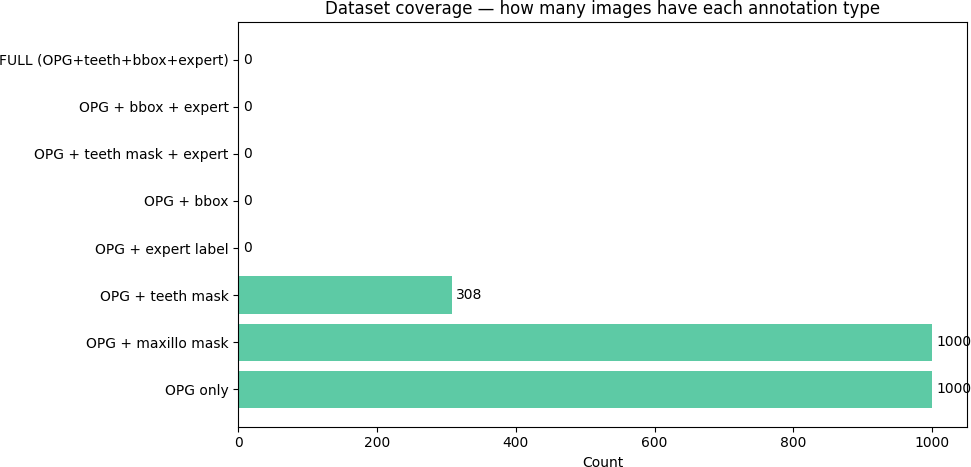
\includegraphics[width=0.66\textwidth]{figures/phase2/p2_4_01_tufts_coverage.png}
\caption[Tufts annotation coverage]{Coverage matrix used to identify the Tufts radiographs that carry
all required annotations (Phase 2 report, Figure 4.1).}
\label{fig:tuftscoverage}
\end{figure}

\section{Evaluation Cohorts}

Table~\ref{tab:cohorts} lists the evaluation populations. All splits are made by image. DENTEX's
disease subset has 250 annotated OPGs; MD5 hashing found 86 of them byte-identical to images the
models trained on (85 in numbering, 1 in detection), leaving 164 scored, of which 148 carry a caries
lesion (479 lesions on 477 teeth). The Ningxia release divides its test data into four sets: test2
comes from the dataset's training centre, and test1, test3 and test4 are described as cross-centre.
These are treated as four sites. % {C060}

\begin{table}[!htbp]
\centering
\caption[Evaluation cohorts]{Evaluation cohorts, units and exposure. Each row is a separate analysis
population; counts are not summed across rows.}
\label{tab:cohorts}
\small
\begin{tabularx}{\textwidth}{@{}L{2.8cm}L{1.4cm}L{4.3cm}Y@{}}
\toprule
Cohort & Images & Unit (n) & Role and exposure\\
\midrule
DENTEX disease & 164 & 936 teeth; 477 carious; 479 lesions & development; the detector trained on other DENTEX images\\
Ningxia, 4 sites & 337 & 1,013 lesions & external; never trained on; informed the lesion detector's adoption\\
CariesXrays & 1,200 & 2,815 lesions & external, except to the lesion detector (its validation split)\\
Tufts test & 143 & 3,760 / 3,892 teeth & numbering / Stage 4 (182 labelled); both trained on Tufts training images\\
UFBA-425 & 425 & 11,591 teeth & numbering; no model trained on it\\
\bottomrule
\end{tabularx}
\end{table}

\section{Data Preparation and Leakage Control}

\subsection{Leakage Control}

\begin{itemize}
\item \textbf{Exact duplicates.} Every evaluation image is hashed (MD5) against every training image;
  the 86 byte-identical DENTEX images are excluded from scoring.
\item \textbf{Near duplicates.} A perceptual-hash search (pHash and dHash) of the 164 scored DENTEX
  images against the 1,389 other DENTEX images checks for re-encoded or resized copies
  (Section~\ref{sec:res-controls}).
\item \textbf{Radiograph-level splits.} Training, validation and test sets are split by radiograph, so
  no radiograph contributes crops to two sets. The Tufts split is frozen and regenerated from code.
\item \textbf{Locked external data.} Ningxia is used only for testing and never for training,
  threshold choice or checkpoint selection.
\end{itemize}

\subsection{Preprocessing Retained from Phase 2}

\textbf{Bounding-box correction.} The raw Tufts annotation stores corners as $[y_1, x_1, y_2, x_2]$,
not $[x, y, w, h]$. Each box is converted with $x = x_1$, $y = y_1$, $w = x_2 - x_1$ and $h = y_2 - y_1$.
Without this correction every crop would have been cut from the wrong place.

\textbf{Asymmetric expanded crop.} For the abnormality flag each tooth box is expanded 1.5 times in
width and 2.0 times in height, clipped to the image and resized to 224 by 224. Teeth on a panoramic
radiograph are much taller than they are wide, so a symmetric expansion would take in neighbouring
teeth while still missing bone below the root.

\textbf{Overlap-ratio labelling.} Intersection over union was rejected for labelling crops, because the
expert masks are sparse and even a genuinely positive crop has an IoU near zero. The label uses the
share of mask pixels inside the crop,
\begin{equation}
\text{overlap} = \frac{\text{non-zero mask pixels inside the crop}}{\text{crop area}},
\label{eq:overlap}
\end{equation}
with a threshold of 0.01 chosen by inspecting the distribution of overlaps
(Figure~\ref{fig:overlapdist}).

\begin{figure}[!htbp]
\centering
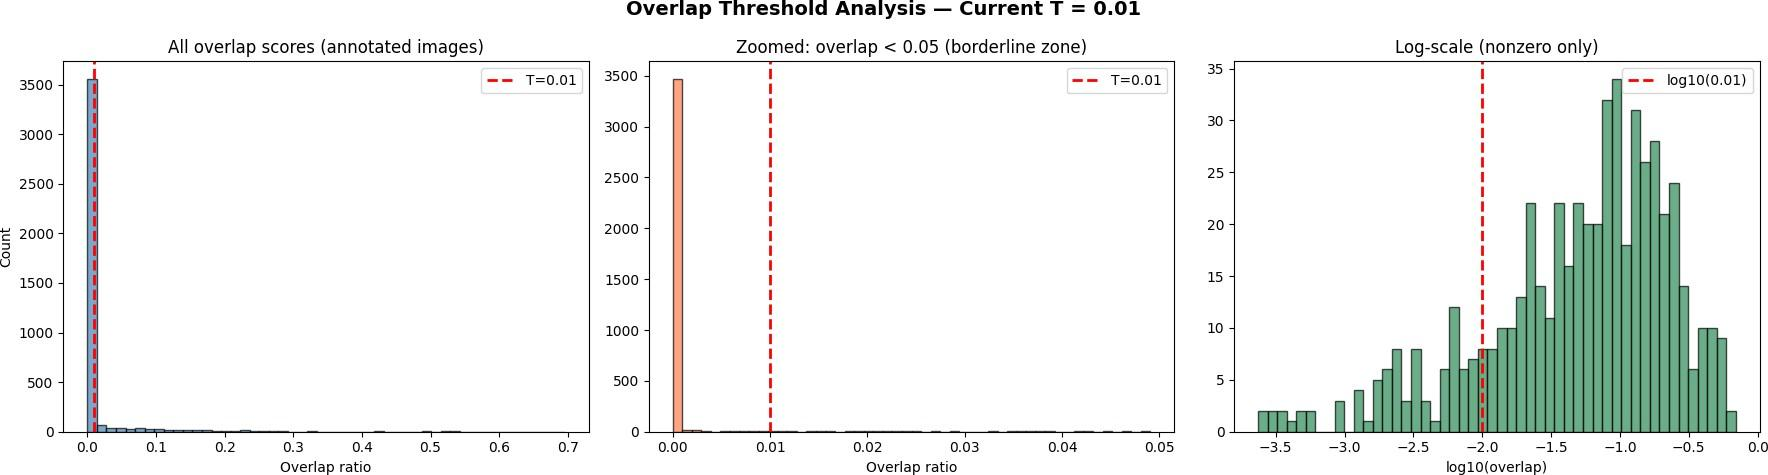
\includegraphics[width=0.8\textwidth]{figures/phase2/p2_4_02_overlap_distribution.jpg}
\caption[Distribution of overlap ratios]{Distribution of overlap ratios used for tooth-level label
assignment (Phase 2 report, Figure 4.2).}
\label{fig:overlapdist}
\end{figure}

\textbf{Box jitter.} A random perturbation of $\pm$15\% is applied to the Tufts boxes during crop
generation, to simulate the localisation noise of a detector and make the classifier less sensitive to
small misalignments. % {C082}

\textbf{CLAHE for the CEJ heuristic.} The exploratory CEJ branch enhanced each crop with
contrast-limited adaptive histogram equalisation (clip limit 2.0, 8 by 8 tiles) and light Gaussian
smoothing; this path is not used by the classifiers.

\textbf{Class imbalance (Phase 2 model).} For the Phase 2 binary model the normal class was
undersampled from 17,473 training crops to 2,500, and the 237 abnormal crops were expanded to 711 by
offline augmentation (random horizontal flip, rotation within 10\textdegree, brightness and contrast
jitter, and a small translation), giving the counts in Table~\ref{tab:p2data}.

\begin{table}[!htbp]
\centering
\caption[Tufts data summary of the Phase 2 binary model]{Tufts data summary of the Phase 2 binary model
(Phase 2 report, Table 4.2). Phase 3 found that this validation split shared radiographs with the
training split (Section~\ref{sec:res-stage4}).}
\label{tab:p2data}
\small
\begin{tabular}{@{}lrrr@{}}
\toprule
Split / subset & Normal & Abnormal & Total\\
\midrule
Raw training crops & 17,473 & 237 & 17,710\\
Resampled training crops & 2,500 & 711 & 3,211\\
Validation crops & 1,499 & 59 & 1,558\\
\bottomrule
\end{tabular}
\end{table}

The Phase 2 report stated that this split was made at the OPG level. The Phase 3 audit found the
opposite: it was a crop-level split, and every one of its validation radiographs also supplied
training crops. That is why the Phase 2 validation figure did not survive a held-out test
(Section~\ref{sec:res-stage4}), and why the Phase 3 model was retrained by radiograph.

\section{Model Training}

All classifier heads are ResNet18 networks pre-trained on ImageNet, with the final layer replaced; the
two detectors are YOLOv11l. Table~\ref{tab:training} gives each shipped model's recipe. Every model
was selected on its own validation split and is a single training run, except Stage~4a, which was
trained with three seeds.

\begin{table}[!htbp]
\centering
\caption[Training recipes of the shipped models]{Training recipes of the shipped models, from each
checkpoint's \texttt{run\_summary.txt}.}
\label{tab:training}
\footnotesize
\begin{tabularx}{\textwidth}{@{}L{2.4cm}L{3.4cm}YL{2.0cm}@{}}
\toprule
Model & Data & Recipe & Kept checkpoint\\
\midrule
Stage 1 detector, YOLOv11l & Tufts + DENTEX + Kaggle, balanced per corpus & 1,024 px, batch 32, AdamW, lr 0.001 with cosine decay, up to 150 epochs (patience 30), mosaic and vertical flip off, seed 42 & best on Tufts validation\\
Stage 2 head, ResNet18 + 4 features & DENTEX + Tufts crops, $1.5\times$ & 224 px, batch 64, lr 0.001 (backbone $\times$0.1), 15 epochs, seed 42 & epoch 12\\
Stage 3a lesion detector, YOLOv11l & 4,800 CariesXrays + 650 DENTEX images (replicated), 9,600 samples per epoch & one class, batch 16, up to 120 epochs (patience 25), mosaic and vertical flip off & epoch 29 of 54\\
Stage 3a crop classifier, ResNet18 & 6,616 tight crops from 260 DENTEX images & 15 epochs, augmented, class weights 3.2849 / 0.5898, seed 42 & epoch 15\\
Stage 3b severity, ResNet18 & DENTEX caries crops & cross-entropy with class weights; Adam, lr 0.001 on the final layer then $3\times10^{-5}$ on the whole network & Phase 2 bundle\\
Stage 4a flag, ResNet18 & 678 Tufts radiographs (36,360 crops) & focal loss ($\gamma$ = 2), Adam lr $10^{-4}$, weight decay $10^{-4}$, batch 32, up to 50 epochs (stop after 10 without gain) & epoch 16 of 26 (seed 42)\\
\bottomrule
\end{tabularx}
\end{table}

Mosaic augmentation and vertical flips are disabled for both detectors by a house rule: a mosaic
breaks the spatial context of a panoramic image, and a vertical flip swaps the upper and lower arches.
Training ran on cloud GPUs and on a laptop accelerator; inference needs neither. % {C083}

\section{The Image-Blind Constant}
\label{sec:method-constant}

\subsection{F1 of a Constant in Closed Form}

Let $N$ images be scored, $P$ be the number of carious teeth over all of them, and $n_c$ the number of
images in which tooth code $c$ is carious, so that $p_c = n_c/N$ is the prevalence of caries at
position $c$. A constant answers the same set $S$ of codes for every image. Its true positives are
$\sum_{c \in S} n_c$ and it names $|S|\,N$ codes, so its micro-averaged F1 is
\begin{equation}
F_1(S) = \frac{2 \sum_{c \in S} n_c}{|S|\,N + P}.
\label{eq:constf1}
\end{equation}
The equation counts every named code as a prediction, present tooth or not, as the scorer does, and
it applies to any set prediction scored by micro-F1 over a fixed label set. Nothing in it depends on an
image. The constant's recall, $\sum_{c \in S} n_c / P$, is the share of carious teeth that lie at its
codes.

\subsection{The Selection Rule}

Write $A = \sum_{c \in S} n_c$ and $k = |S|$. Adding a code $c \notin S$ raises the score,
$2(A+n_c)/((k+1)N+P) > 2A/(kN+P)$, if and only if
\begin{equation}
p_c > \tfrac{1}{2}\, F_1(S).
\label{eq:rule}
\end{equation}
For any fixed size the best set is the $k$ most prevalent codes, so the F1-optimal constant is a
prefix of the codes sorted by prevalence. Writing $S_k$ for the $k$ most prevalent codes, F1 rises
along $S_1, S_2, \dots$ to a single peak: if code $k+1$ fails~\eqref{eq:rule} against $S_k$, then
$p_{k+1} \le \tfrac{1}{2}F_1(S_{k+1})$ as well, so every later, less prevalent code fails too. The
optimum is the prefix cut where~\eqref{eq:rule} first fails, and it holds exactly the codes with
$p_c > \tfrac{1}{2}F_1^{*}$: a functional of the caries prior alone. That first molars are the most
caries-susceptible teeth is long established in caries epidemiology~\cite{batchelor2004grouping}; the
prior, and with it the floor, depends on the population's age and exposure. % {C010}

The constant is fitted on the 78 DENTEX images that were excluded from scoring because the models
trained on them, and frozen before it is scored (Figure~\ref{fig:prior}). % {C010}

\begin{figure}[!htbp]
\centering
\includegraphics[width=0.94\textwidth]{figures/repo/R05_positional_prior.pdf}
\caption[The positional prior and the constant it implies]{The positional prior and the constant it
implies. (a) Share of images in which the expert marked each FDI code carious, in chart order
(patient's right to left, as displayed): grey, the fit set (78 DENTEX images with caries, excluded from
scoring because the models trained on them); orange, the 164 scored images. Magenta: the eight codes
rule~\eqref{eq:rule} admits; dashed: the final threshold $F_1/2 = 0.196$. (b) F1 of the $k$ most
prevalent fit-set codes.}
\label{fig:prior}
\end{figure}

\subsection{Lesion Agreement and the Cohort's Prior}

The second metric family scores lesions rather than codes. Let a cohort contain $L$ expert lesions,
let $T(\ell)$ be the detected tooth that contains lesion $\ell$, and let $\mathcal{F}$ be the set of
teeth a system flags. Lesion agreement is
\begin{equation}
A(\mathcal{F}) = \frac{1}{L} \sum_{\ell} \mathbf{1}\big[\, T(\ell) \in \mathcal{F} \,\big].
\label{eq:agreement}
\end{equation}
It has no negative class, so it can only rise as $\mathcal{F}$ grows, and flagging every detected tooth
reaches its ceiling, the share of lesions inside any detected tooth; it must be read beside the number
of teeth flagged. For the constant, $\mathcal{F}$ is the eight molar boxes the front end finds, so $A$
is the cohort's prior mass on those molars. That prior mass varies between cohorts and between sites
of one cohort, as Zech et al.\ found for pneumonia prevalence between hospitals~\cite{zech2018variable},
so systems can be compared only when paired on the same images, cohort by cohort and site by site.

\section{A Test for a Positional Shortcut}

If a per-tooth classifier has learned the probability of caries given position, and not only given
pixels, two consequences follow. Its score on truly healthy teeth should rise with the base rate of
their position, because the prior lifts every tooth of a caries-prone type. And its ranking should
survive only partly when position is held fixed: the within-type area under the ROC curve (AUC), which
ranks carious against healthy teeth of the same type, removes the positional cue and keeps the image
signal. Both tests are applied to the crop classifier on 863 held-out tooth crops from 34 radiographs,
cut with ground-truth boxes so that the front end plays no part (Section~\ref{sec:res-shortcut}).

A whole-image lesion detector receives no tooth identity: to flag a tooth it must place a box mostly
inside it. It can express a positional prior only by drawing boxes over molars where it sees no lesion,
and each such box costs precision under~\eqref{eq:constf1} and earns agreement
under~\eqref{eq:agreement} only if a lesion happens to lie there. If the detector's lead over the
constant comes from reading the image, it should therefore come with fewer flagged teeth, and within
each tooth type its flags should be carious more often than the classifier's. % {C093}

\section{Evaluation Protocol}
\label{sec:method-eval}

\subsection{Systems Compared}

Four systems answer one question, which teeth in this radiograph show caries, on the same 164 images:
the pipeline (with each Stage-3a method), Qwen2.5-VL-32B (33.45\,B parameters) and Qwen2.5-VL-7B
(8.29\,B), both zero-shot with the FDI scheme in the prompt and also shown a blank grey and a
random-noise image as content-free controls, and the image-blind constant.

\subsection{Metrics}

FDI-set F1~\eqref{eq:constf1} is micro-averaged over teeth. Lesion agreement~\eqref{eq:agreement}
matches each expert lesion to a flagged tooth. On DENTEX it uses a greedy intersection over union of at
least 0.30 with a centroid fallback. On the external cohorts it uses centroid containment, because their
lesions are small (median 731 pixels) inside tooth boxes of about 25,000 pixels, so every comparison is
made within a cohort. % {C094}

\subsection{Statistics}

Teeth within one radiograph share exposure, anatomy and annotator, so their errors are correlated. All
intervals are 95\% percentile bootstrap confidence intervals (CI) over images, not teeth, the cluster bootstrap that stays
consistent when clusters carry random effects~\cite{field2007bootstrapping}. Unless stated, 10,000
resamples with seed 42 are used; the crop classifier's calibration average precision (AP) uses 2,000, its within-type AUC
5,000, and the two abstention gains 1,000 with seed 0. For two systems scored on the same images, the
paired difference is recomputed on every resample, and its 2.5th and 97.5th percentiles give the
interval. Differences are system minus comparator in percentage points (pp). % {C095}

Across the four Ningxia sites, the per-site differences $\Delta_j$ with variances $v_j$ (from each
site's interval width) are pooled by DerSimonian--Laird random effects~\cite{dersimonian1986meta},
\begin{equation}
\hat\mu = \frac{\sum_j \Delta_j / (v_j + \hat\tau^2)}{\sum_j 1 / (v_j + \hat\tau^2)},
\label{eq:dl}
\end{equation}
where the between-site variance $\hat\tau^2$ is estimated from Cochran's $Q$, and
$I^2 = (Q - k + 1)/Q$ is the share of variation due to sites~\cite{higgins2002quantifying}. A fixed-site
interval asks whether a system led at these sites; the random-effects prediction interval asks whether
it would lead at another~\cite{riley2011interpretation}. With only four sites the DerSimonian--Laird
interval is too narrow, so the Hartung--Knapp--Sidik--Jonkman (HKSJ) interval~\cite{inthout2014hartung}
and a Q-profile interval for $\tau$~\cite{viechtbauer2007confidence} are reported beside it.

\subsection{Matched-Volume Comparison}

A system that names more teeth than the constant can buy F1 with volume. Each system is therefore also
compared with an image-blind answer that names exactly as many codes: the $k$ most prevalent fit-set
codes on some images and the $k+1$ most prevalent on the rest, a mixture chosen without looking at any
image, whose true positives and named codes are linear in the mixing fraction.

\subsection{Estimation, Not Testing}

Results are reported as estimates with intervals, not as a family of hypothesis tests, so no
multiplicity correction is applied across cohorts, arms, metrics and sites. The theory of
Section~\ref{sec:method-constant} was formulated after the measurements it is checked against, so its
check in Chapter~\ref{ch:results} is a consistency check, not a test of predictions made in advance.

\section{Pre-Registration and Experiment Governance}
\label{sec:method-prereg}

Changes to a default checkpoint were proposed as numbered ``levers'', each with an acceptance rule
committed before the arm was trained (Table~\ref{tab:levers}, Figure~\ref{fig:levers}). The caries
reformulation's rule, committed as \texttt{ef3f453} before any arm was trained, required the lesion
detector to beat both the image-blind constant and the crop classifier on at least two of three
cohorts, with the interval excluding zero, at no more than 1.5 times their rate of flagged teeth.
Because Ningxia was one of the three cohorts, it informed the adoption, and the lead measured on it is
optimistic by construction. % {C021}

\begin{table}[!htbp]
\centering
\caption[Levers attempted and their outcomes]{Levers attempted and their outcomes.}
\label{tab:levers}
\small
\begin{tabularx}{\textwidth}{@{}L{1.0cm}L{4.4cm}Y@{}}
\toprule
Lever & Change & Outcome\\
\midrule
1 & Multi-corpus detector (Tufts + DENTEX) & DENTEX numbering rose sharply; the Tufts guard failed: kept as an ablation\\
2 & Stand-alone CariesXrays lesion detector & Level with the benchmark's own method; a benchmark row, not a pipeline component\\
A & Multi-corpus detector, three- and four-corpus arms, balanced per corpus & Primary metric and external-caries guard passed; the Tufts box mAP guard failed: an ablation, the three-corpus arm later made the default by a separate decision\\
A2 & Frozen-backbone Tufts fine-tune of Lever A & Tufts test guard still failed: an ablation\\
B & Caries as whole-image lesion detection & Met the rule on two of three cohorts: \textbf{adopted}\\
C & Structural FDI post-processing & Null: not adopted\\
\bottomrule
\end{tabularx}
\end{table}

\begin{figure}[!htbp]
\centering
% Experiment lineage. Traced to transfer.md section 2.6 (levers 1, 2, A, A2, B, C) and models/README.md.
\begin{tikzpicture}[node distance=5mm and 7mm,
  lev/.style={box,fill=#1,text width=32mm,minimum height=10mm,font=\sffamily\tiny\bfseries}]
\node[io,text width=32mm] (base) {Phase 2 modules\\[-1pt]{\normalfont crop classifier, Tufts-only detector}};
\node[lev=p2arrow,right=of base,yshift=13mm] (l1) {Lever 1: multi-corpus detector\\[-1pt]{\normalfont Tufts guard failed}};
\node[lev=p2orange,right=of l1] (la) {Lever A: 3- and 4-corpus detector\\[-1pt]{\normalfont arm 3C made default, 11 Oct}};
\node[lev=p2arrow,right=of la] (la2) {Lever A2: frozen fine-tune\\[-1pt]{\normalfont Tufts guard failed}};
\node[lev=p2arrow,right=of base,yshift=-1mm] (l2) {Lever 2: CariesXrays detector\\[-1pt]{\normalfont benchmark row}};
\node[lev=p2green,right=of l2] (lb) {Lever B: lesion detector\\[-1pt]{\normalfont adopted 4 Sep, 2 of 3 cohorts}};
\node[lev=p2arrow,right=of base,yshift=-15mm] (rep) {Five crop-classifier repairs\\[-1pt]{\normalfont none separated from zero}};
\node[lev=p2arrow,right=of rep] (lc) {Lever C: FDI structural repair\\[-1pt]{\normalfont null}};
\node[lev=p2green,right=of lc] (s4) {Stage 4a by radiograph\\[-1pt]{\normalfont default 13 Oct}};
\draw[arr] (base.east) -- ++(2mm,0) |- (l1.west); \draw[arr] (l1) -- (la); \draw[arr] (la) -- (la2);
\draw[arr] (base.east) -- ++(2mm,0) |- (l2.west); \draw[arr] (l2) -- node[lbl,above]{same arch.} (lb);
\draw[arr] (base.east) -- ++(2mm,0) |- (rep.west); \draw[arr] (rep) -- (lc);
\draw[darr] (rep.north) -- node[lbl,right]{task changed} (lb.south west);
\end{tikzpicture}

\caption[Experiment lineage]{Experiment lineage. Green: adopted into the pipeline; grey: ablation or
null; orange: adopted by a separate decision against a failed guard.}
\label{fig:levers}
\end{figure}

\chapter{Implementation and Pseudocode}
\label{ch:impl}

\section{Technology Stack}

The implementation is in Python 3.12. PyTorch and torchvision run the ResNet18 heads; Ultralytics
YOLO11 trains and runs the two detectors; OpenCV and NumPy cut crops and process masks; SciPy supplies
the linear-assignment solver for numbering; pandas joins annotations; scikit-learn computes metrics and
fits the isotonic calibrator; Matplotlib draws the figures; Streamlit serves the demo; pytest runs the
tests; and Docker packages the demo. Exact versions are pinned in \texttt{requirements-lock.txt}
(Table~\ref{tab:hwsw}). NumPy is held below version 2, which breaks the SciPy import that the
Hungarian assignment needs.

\section{Repository Structure}

The repository layout, to two levels, is shown in Figure~\ref{fig:repotree}.

\begin{figure}[!htbp]
\centering
% Repository structure (top levels). Traced to `git ls-files` of the repository on 2 Nov 2026.
\begin{minipage}{0.92\textwidth}
\small
\renewcommand{\DTstyle}{\ttfamily\small}
\renewcommand{\DTcomment}{\rmfamily\itshape\color{p2grey}}
\dirtree{%
.1 An-Intelligent-Dental-Assisting-System/.
.2 app.py\DTcomment{Streamlit web demo}.
.2 Dockerfile\DTcomment{CPU-only container with a build self-test}.
.2 src/\DTcomment{reusable stage modules (orientation, numbering, classifiers, crops)}.
.2 scripts/.
.3 run\_inference.py\DTcomment{Stages 5--6: one OPG in, one JSON report out}.
.3 eval/\DTcomment{40 evaluation scripts}.
.3 dentex/, tufts/, yolo/\DTcomment{dataset builders and trainers}.
.3 figures/\DTcomment{figure scripts with asserted values}.
.3 verify\_paper\_numbers.py\DTcomment{asserts 215 reported numbers}.
.2 models/\DTcomment{one folder per trained stage, with run summaries}.
.2 outputs/\DTcomment{saved evaluation results (JSON, CSV)}.
.2 tests/\DTcomment{23 test modules}.
.2 notebooks/\DTcomment{Phase 2 development notebooks}.
.2 docs/\DTcomment{results log, model metrics, session memory}.
.2 paper/\DTcomment{manuscript and the ten-page IEEE draft}.
.2 requirements.txt, requirements-lock.txt\DTcomment{dependencies}.
}
\end{minipage}

\caption[Repository structure]{Repository structure (top two levels, main folders only).}
\label{fig:repotree}
\end{figure}

The working rules of the repository are part of the implementation. Every result is logged in a
dated, append-only results log. Every default checkpoint is pinned by hash. Superseded checkpoints are
kept, not deleted, so that earlier numbers stay reproducible. Large raw data stay outside version
control.

\section{Modules Carried Over from Phase 2}

\subsection{Module 1: Caries Cascade}

The Phase 2 caries work is a two-stage cascade rather than one three-class model. The first stage, a
ResNet18 on tight tooth crops resized to 224 by 224 with ImageNet normalisation, predicts caries
against no caries; the second reuses the backbone for caries against deep caries, with the final layer
reset and the network fine-tuned at a lower learning rate so that it adapts to severity cues. In
Phase 3 the first stage was retrained with a real negative class of 5,366 healthy teeth, becoming the
retained crop classifier, and the second stage is the shipped severity grader (Stage~3b). % {C084}

\subsection{Module 2: Dataset Exploration and Annotation Parsing}

\texttt{src/data\_loader.py} turns the raw Tufts annotations into a form suitable for tooth-level
analysis. Three parsing bugs were decisive in Phase 2:
\begin{itemize}
\item the expert and box files are lists of records keyed by the stem of their External ID, not
  dictionaries keyed by image name;
\item the boxes are stored as $[y_1, x_1, y_2, x_2]$;
\item the mask values encode lesion instances, not severity classes.
\end{itemize}
The module therefore loads the expert descriptions and derives the image stems, converts the boxes to
$[x, y, w, h]$, classifies each mask as empty or annotated, and joins all sources on the stem.

\subsection{Module 3: Abnormality Dataset Construction}

\texttt{src/crop\_generator.py} and \texttt{src/label\_assigner.py} build the expanded crop from a tooth
box, optionally jitter it, crop the expert mask to the same region and compute the overlap
ratio~\eqref{eq:overlap} that sets the label. This turns sparse region annotations into a tooth-wise
label without lesion segmentation at inference (Figures~\ref{fig:p2grid} and~\ref{fig:p2samples}).

\begin{figure}[!htbp]
\centering
\optionalgraphics[width=0.66\textwidth]{figures/phase2/p2_5_01_crop_validation_grid.jpg}
\caption[Validation grid of tooth boxes, expanded crops and mask-aligned crops]{Validation grid of
tooth boxes, expanded crops and mask-aligned crops (Phase 2 report, Figure 5.1). Tufts radiographs.}
\label{fig:p2grid}
\end{figure}

\begin{figure}[!htbp]
\centering
\optionalgraphics[width=0.86\textwidth]{figures/phase2/p2_5_02_crop_samples.jpg}
\caption[Representative tooth crops of the abnormality dataset]{Representative tooth crops of the
abnormality dataset (Phase 2 report, Figure 5.2). Tufts radiographs.}
\label{fig:p2samples}
\end{figure}

One limitation noted in Phase 2 remains true: the abnormal pool contained jittered near-duplicates of
the same teeth, and offline augmentation multiplied them. The Phase 3 retrain replaced offline
augmentation with an epoch that draws every abnormal crop once and 3.5 normal crops for each, redrawn
every epoch.

\subsection{Modules 4 and 5: Binary Flag and Severity Training}

The Phase 2 binary model fine-tuned a ResNet18 on the expanded crops with focal loss, Adam,
learning-rate reduction on plateau and early stopping; its best epoch was 22. The Phase 2 severity
model was a three-class ResNet18 trained with focal loss on the positive crops. Phase 3 kept both
recipes and changed the split (Section~\ref{sec:sys-stage4}). % {C085}

\subsection{Module 6: CEJ-Based Estimation}

The CEJ heuristic used CLAHE preprocessing, column-wise CEJ and apex detection, a focused search window
for the bone crest, interquartile-range outlier removal and a confidence score
(Figure~\ref{fig:p2cej}). Its results are in Section~\ref{sec:sys-stage4}. % {C086}

\begin{figure}[!htbp]
\centering
\optionalgraphics[width=0.66\textwidth]{figures/phase2/p2_5_03_cej_overlays.jpg}
\caption[CEJ-estimation overlays on tooth crops]{CEJ-estimation overlays on tooth crops from the
exploratory branch (Phase 2 report, Figure 5.3). Tufts radiographs.}
\label{fig:p2cej}
\end{figure}

\section{Modules Added in Phase 3}

\begin{description}[leftmargin=0pt,style=nextline]
\item[Module 7: Tooth detector.] Dataset builders under \texttt{scripts/yolo/} convert each corpus to
  the YOLO format in the detector's rotated frame, balance the corpora and train with Ultralytics.
\item[Module 8: Numbering head.] \texttt{scripts/dentex/build\_enumeration\_crops.py} builds the
  $1.5\times$ crops and box features from DENTEX and Tufts, splitting by source image before any crop
  exists, and \texttt{train\_enumeration\_head.py} trains the two-headed ResNet18.
\item[Module 9: Lesion detector.] \texttt{build\_dentex\_caries\_boxes.py} converts the 705 DENTEX
  disease images into single-class lesion boxes (650 kept), pooled with CariesXrays, with a live MD5
  check against the scored cohort.
\item[Module 10: Integration.] \texttt{scripts/run\_inference.py} composes the stages
  (Algorithm~\ref{alg:pipeline}) and writes the report.
\item[Module 11: Web demo and container.] \texttt{app.py} renders the report in a browser, and the
  Dockerfile packages it with a build-time self-test.
\item[Module 12: Evaluation suite.] Forty scripts under \texttt{scripts/eval/} reproduce every result:
  lesion agreement on DENTEX, Ningxia and CariesXrays; the vision-language and constant baselines;
  numbering, abstention and calibration; the shortcut test; random-effects pooling; constant
  stability; and the near-duplicate check.
\end{description}

\section{Pseudocode}

Eight algorithms give the pseudocode of the pipeline and of the evaluation: end-to-end inference
(Algorithm~\ref{alg:pipeline}), one-to-one FDI assignment (Algorithm~\ref{alg:fdi}), lesion-to-tooth
assignment (Algorithm~\ref{alg:lesion}), the fit of the image-blind constant
(Algorithm~\ref{alg:constant}), the paired cluster bootstrap (Algorithm~\ref{alg:bootstrap}), the
matched-volume comparison (Algorithm~\ref{alg:matched}), random-effects pooling across sites
(Algorithm~\ref{alg:re}) and the near-duplicate check (Algorithm~\ref{alg:nearDup}).

\begin{algorithm}[!htbp]
\caption{End-to-end inference (\texttt{run\_pipeline})}
\label{alg:pipeline}
\begin{algorithmic}[1]
\Require OPG image $I$; loaded models; caries method $m \in \{\text{lesion-detector}, \text{gate}\}$
\Ensure report $R$
\State $W \gets \textsc{CheckInput}(I)$ \Comment{warnings, never a silent failure}
\State $(B, s) \gets \textsc{DetectUpright}(\text{detector}, I)$ \Comment{rotate 90\textdegree, detect at 1,024 px, conf.\ 0.25, NMS 0.50, rotate back}
\State $(c, q) \gets \textsc{AssignFDI}(\text{head}, I, B)$ \Comment{Algorithm~\ref{alg:fdi}}
\If{$m = \text{lesion-detector}$}
  \State $K \gets \textsc{LesionCaries}(I, B)$ \Comment{Algorithm~\ref{alg:lesion}}
\Else
  \State $K \gets \textsc{GateCaries}(I, B)$ \Comment{tight crops, ResNet18, then severity}
\EndIf
\State $A \gets \textsc{AbnormalityFlag}(I, B)$ \Comment{$1.5\times2.0$ crops, ResNet18}
\State \textbf{assert} $|B| = |c| = |K| = |A|$ \Comment{refuse to fuse misaligned outputs}
\For{each tooth $i$}
  \State $\text{assessable}_i \gets (c_i \neq \varnothing) \wedge (q_i \geq 0.30)$
\EndFor
\State $R \gets \textsc{BuildReport}(B, s, c, q, K, A, W)$; sort records by FDI code
\State attach checkpoint hashes, runtime versions and the limitations of the checkpoints that ran
\State \Return $R$
\end{algorithmic}
\end{algorithm}

\begin{algorithm}[!htbp]
\caption{One-to-one FDI assignment (\texttt{assign\_fdi\_head})}
\label{alg:fdi}
\begin{algorithmic}[1]
\Require image $I$ of width $W$ and height $H$; tooth boxes $b_1,\dots,b_n$; two-headed network $g$
\For{$i = 1$ to $n$}
  \State $x_i \gets \textsc{Resize}(\textsc{Crop}(I, \textsc{Expand}(b_i, 1.5, 1.5)), 224)$
  \State $f_i \gets (c_x/W,\ c_y/H,\ w/W,\ h/H)$ of $b_i$
\EndFor
\State $(\ell^{q}, \ell^{p}) \gets g(x, f)$ \Comment{log-softmax over 4 quadrants and 8 positions}
\State $J_{i,(Q,P)} \gets \ell^{q}_{i,Q} + \ell^{p}_{i,P}$ for all 32 codes \Comment{joint log-probability}
\If{any $J$ is not finite} \State \textbf{raise} an error \EndIf
\State $\pi \gets \textsc{LinearSumAssignment}(-J)$ \Comment{Hungarian: maximise $\sum_i J_{i,\pi(i)}$, one code per tooth}
\For{$i = 1$ to $n$}
  \State $c_i \gets \pi(i)$, or none if more than 32 teeth were detected and $i$ is unmatched
  \State $q_i \gets \exp(J_{i,c_i})$; flag $c_i$ as doubtful if $q_i < 0.30$
\EndFor
\State \Return $(c, q)$
\end{algorithmic}
\end{algorithm}

\begin{algorithm}[!htbp]
\caption{Lesion-to-tooth assignment (\texttt{run\_caries\_lesion\_detector})}
\label{alg:lesion}
\begin{algorithmic}[1]
\Require upright image $I$; tooth boxes $b_1,\dots,b_n$; lesion detector $D$; severity network $h$
\State $\mathcal{L} \gets D(I)$ at 1,024 px, confidence $\geq 0.25$ \Comment{no rotation: trained upright}
\State $\text{best} \gets \{\}$
\For{each lesion box $l$ with score $\sigma$ in $\mathcal{L}$}
  \State $r_i \gets \text{area}(l \cap b_i) / \text{area}(l)$ for every tooth $i$ \Comment{containment}
  \If{$\max_i r_i > 0$}
    \State $i^{*} \gets \arg\max_i r_i$
    \State $\text{best}[i^{*}] \gets \max(\text{best}[i^{*}], \sigma)$ \Comment{one tooth per lesion}
  \EndIf \Comment{a lesion outside every tooth is dropped}
\EndFor
\For{each tooth $i$}
  \If{$i \in \text{best}$}
    \State severity $\gets h(\textsc{TightCrop}(I, b_i))$; finding $\gets$ caries or deep caries
  \Else
    \State finding $\gets$ no caries
  \EndIf
\EndFor
\State \Return one finding per tooth, with the detection score marked as such
\end{algorithmic}
\end{algorithm}

\begin{algorithm}[!htbp]
\caption{Fitting the image-blind constant (rule~\eqref{eq:rule})}
\label{alg:constant}
\begin{algorithmic}[1]
\Require fit images, $N$ of them, with carious codes; $n_c$ = images with code $c$ carious; $P = \sum_c n_c$
\State order the 32 codes by $n_c$, largest first
\State $S \gets \varnothing$; $A \gets 0$
\For{each code $c$ in that order}
  \State $k \gets |S|$
  \If{$n_c > 0$ \textbf{and} $2(A + n_c)(kN + P) > 2A((k+1)N + P)$} \Comment{adding $c$ raises F1}
    \State $S \gets S \cup \{c\}$; $A \gets A + n_c$
  \Else
    \State \textbf{break} \Comment{single peak: every later code fails too}
  \EndIf
\EndFor
\State \Return $S$, frozen before it is scored
\end{algorithmic}
\end{algorithm}

\begin{algorithm}[!htbp]
\caption{Paired cluster bootstrap}
\label{alg:bootstrap}
\begin{algorithmic}[1]
\Require images $1,\dots,N$; per-image counts for systems $X$ and $Y$; metric $M$; $R = 10{,}000$; seed 42
\For{$r = 1$ to $R$}
  \State draw $N$ image indices with replacement \Comment{resample radiographs, not teeth}
  \State $\Delta_r \gets M_X(\text{draw}) - M_Y(\text{draw})$ \Comment{both systems on the same draw}
\EndFor
\State \Return point estimate on all images; interval $[\Delta_{(2.5\%)}, \Delta_{(97.5\%)}]$
\end{algorithmic}
\end{algorithm}

\begin{algorithm}[!htbp]
\caption{Matched-volume image-blind comparison}
\label{alg:matched}
\begin{algorithmic}[1]
\Require system predictions on $N$ images; fit-set prevalence order of codes; $P$ carious teeth
\State $v \gets (\text{codes the system names}) / N$; $k \gets \lfloor v \rfloor$; $f \gets v - k$
\For{each image $j$}
  \State $\mathit{TP}^{\text{mix}}_j \gets (1-f)\,\mathit{TP}_j(S_k) + f\,\mathit{TP}_j(S_{k+1})$ \Comment{mixture chosen by image ID, not content}
\EndFor
\State $F_1^{\text{mix}} \gets 2\sum_j \mathit{TP}^{\text{mix}}_j / (vN + P)$
\State $\Delta \gets F_1^{\text{system}} - F_1^{\text{mix}}$; interval by Algorithm~\ref{alg:bootstrap} with $f$ fixed
\State \Return $\Delta$ and its interval
\end{algorithmic}
\end{algorithm}

\begin{algorithm}[!htbp]
\caption{Random-effects pooling across sites, with HKSJ and Q-profile intervals}
\label{alg:re}
\begin{algorithmic}[1]
\Require per-site differences $\Delta_j$ and 95\% intervals $[l_j, u_j]$, $j = 1,\dots,k$
\State $v_j \gets ((u_j - l_j)/3.92)^2$; $w_j \gets 1/v_j$
\State $Q \gets \sum_j w_j (\Delta_j - \bar\Delta_w)^2$; $\hat\tau^2 \gets \max\!\big(0, \frac{Q-(k-1)}{\sum w_j - \sum w_j^2/\sum w_j}\big)$ \Comment{DerSimonian--Laird}
\State $w^{*}_j \gets 1/(v_j + \hat\tau^2)$; $\hat\mu \gets \sum w^{*}_j \Delta_j / \sum w^{*}_j$
\State DL interval: $\hat\mu \pm 1.96\,(\sum w^{*}_j)^{-1/2}$
\State $q \gets \sum w^{*}_j(\Delta_j - \hat\mu)^2/(k-1)$; HKSJ interval: $\hat\mu \pm t_{k-1}\sqrt{q/\sum w^{*}_j}$
\State Q-profile: solve $Q(\tau^2) = \chi^2_{k-1}$ quantiles for the bounds of $\tau^2$
\State prediction interval: $\hat\mu \pm t_{k-2}\sqrt{\hat\tau^2 + \text{SE}^2}$
\State \Return $\hat\mu$, DL and HKSJ intervals, $\tau$ interval, $I^2$, prediction interval
\end{algorithmic}
\end{algorithm}

\begin{algorithm}[!htbp]
\caption{Near-duplicate check (\texttt{dentex\_near\_duplicates.py})}
\label{alg:nearDup}
\begin{algorithmic}[1]
\Require query images (scored cohort); reference images (all other DENTEX images)
\For{each image $x$}
  \State pHash$(x)$: 32$\times$32 greyscale, 2-D DCT, top-left 8$\times$8 thresholded at its median (64 bits)
  \State dHash$(x)$: 9$\times$8 greyscale, sign of the horizontal gradient (64 bits)
\EndFor
\State Hamming distance from every query to every reference, for both hashes
\State positive control: every MD5-identical pair must be at distance 0 under both hashes
\State candidates $\gets$ queries with pHash distance $\leq 6$ or dHash distance $\leq 4$
\State inspect each candidate beside its nearest neighbours by eye; record the verdict
\end{algorithmic}
\end{algorithm}

\section{Verification and Testing}
\label{sec:impl-verify}

The code and the reported numbers were checked in six ways, summarised in Table~\ref{tab:verify}. % {C050}

\begin{table}[!htbp]
\centering
\caption[Verification results]{Verification results of the code and of the reported numbers, re-run
on 6 November 2026 unless stated.}
\label{tab:verify}
\small
\begin{tabularx}{\textwidth}{@{}L{4.0cm}YL{3.4cm}@{}}
\toprule
Check & What it verifies & Result\\
\midrule
Unit and integration tests & 23 modules, including an end-to-end pipeline run & 210 passed, 3 skipped\textsuperscript{a}\\
Number verification & 215 manuscript numbers asserted against their saved artefacts & 215 of 215, no drift\\
Number trace (2 Nov) & every number in the ten-page paper draft traced to a file & 390 numbers; 6 untraced, each explained\\
Invariants & twelve properties of the saved outputs, such as the 86-image exclusion list & 12 of 12 hold\\
Citation audit & every reference resolved on Crossref, OpenAlex, Semantic Scholar or arXiv & verified\\
Container build & imports, the Hungarian solver and the NumPy version, at build time & build self-test\\
\bottomrule
\end{tabularx}
\srcnote{\textsuperscript{a}\,The three skipped tests need the raw Tufts radiographs, which are not on
the machine that ran them.}
\end{table}

\section{Deployment}

The demo container is built with \texttt{docker build -t opg-pipeline .} and run with
\texttt{docker run -p 8501:8501 opg-pipeline}; the page opens at \texttt{http://localhost:8501}. The
build installs the CPU wheel of PyTorch and fails if a dependency would break the pipeline. The running
container is health-checked every 30 seconds. Appendix~B gives the full instructions.

\chapter{Experimentation, Results and Discussion}
\label{ch:results}

This chapter first revisits the Phase 2 results, because two of them did not survive Phase 3. It then
reports the training diagnostics, the identity factors, the image-blind constant, and the answers to
RQ1--RQ3. It ends with the abnormality flag, the controls, runtime, a discussion and the limitations.
Unless stated otherwise, intervals are 95\% paired cluster-bootstrap intervals over images, and
differences are system minus comparator in percentage points. % {C095}

\section{Phase 2 Results Revisited}
\label{sec:res-phase2}

The Phase 2 report presented the results in Table~\ref{tab:p2results} and
Figures~\ref{fig:p2train}--\ref{fig:p2cejagree}. They are kept here as they were measured, and
Table~\ref{tab:p2corrections} states what Phase 3 found about each.

\begin{table}[!htbp]
\centering
\caption[Phase 2 results as reported]{Phase 2 results as reported (Phase 2 report, Tables 6.1 and
6.2), all on validation splits.}
\label{tab:p2results}
\small
\begin{tabularx}{\textwidth}{@{}L{4.0cm}YYL{3.6cm}@{}}
\toprule
Module & Headline & Other figures & Evaluation set\\
\midrule
Bone-loss binary & macro-F1 0.9233 & sensitivity 0.8305, specificity 0.9953 & 1,558 validation crops\\
Bone-loss severity & macro-F1 0.7208 & mild-class F1 0.80 & positive subset (mild $n = 6$)\\
Caries severity (final cascade run) & macro-F1 0.77 & accuracy 0.81, deep-caries recall 0.84 & 133 validation crops\\
CEJ heuristic & reliable on 62.5\% & exact agreement 15.1\%, within one class 61.6\% & 296 crops\\
\bottomrule
\end{tabularx}
\end{table}

\begin{figure}[!htbp]
\centering
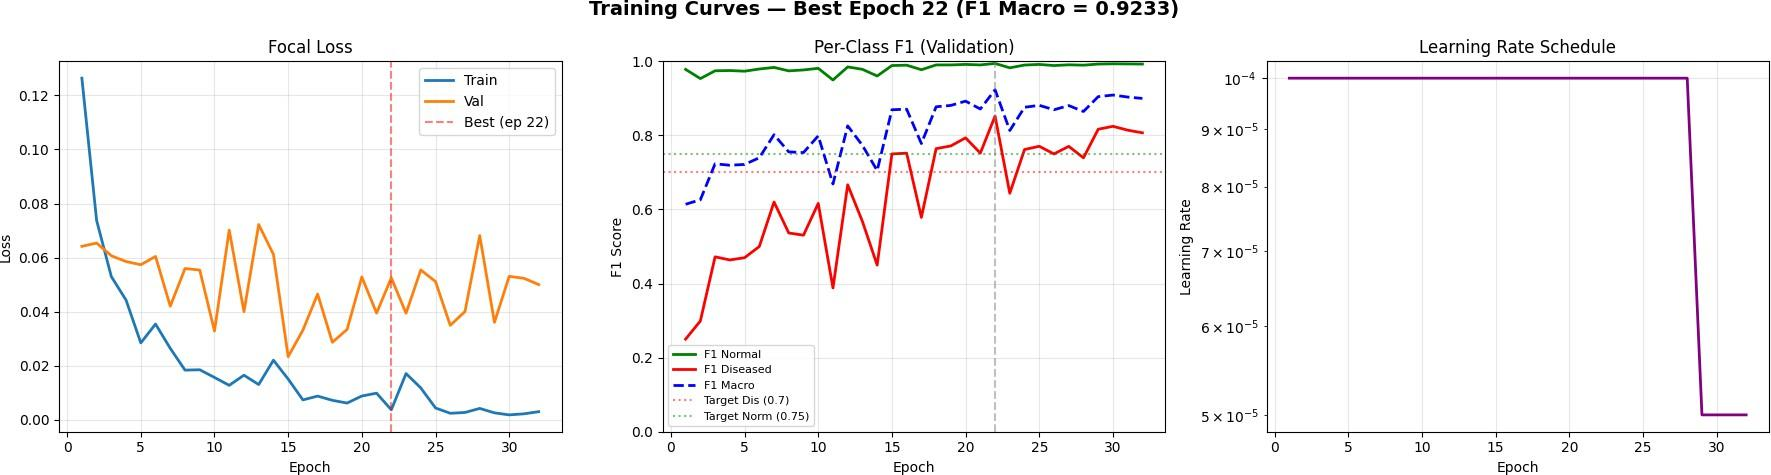
\includegraphics[width=0.92\textwidth]{figures/phase2/p2_6_01_boneloss_training.jpg}
\caption[Phase 2 training curves of the binary bone-loss classifier]{Training and validation curves of
the Phase 2 binary bone-loss classifier (Phase 2 report, Figure 6.1). Its validation split shared
radiographs with training; see Table~\ref{tab:p2corrections}.}
\label{fig:p2train}
\end{figure}

\begin{figure}[!htbp]
\centering
\begin{subfigure}[b]{0.56\textwidth}
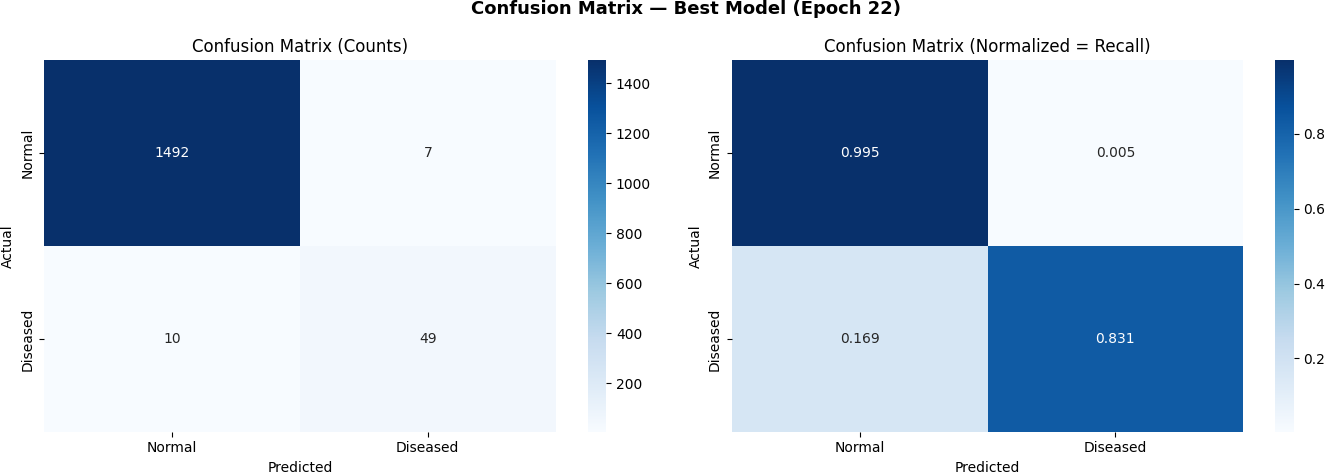
\includegraphics[width=\textwidth]{figures/phase2/p2_6_02_boneloss_confusion.png}
\caption{Binary model, validation split.}
\label{fig:p2cm}
\end{subfigure}\hfill
\begin{subfigure}[b]{0.42\textwidth}
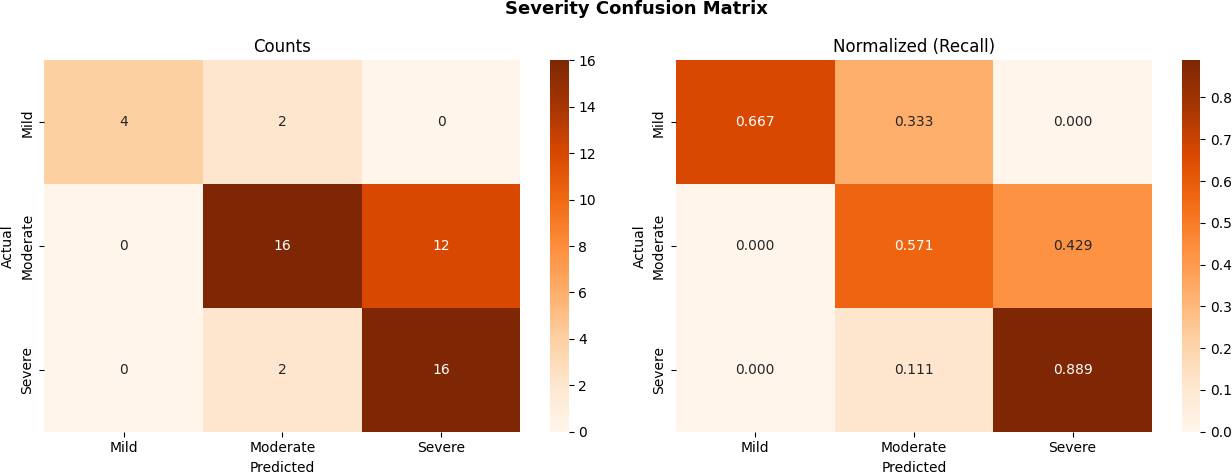
\includegraphics[width=\textwidth]{figures/phase2/p2_6_03_severity_confusion.png}
\caption{Severity model, positive subset.}
\label{fig:p2sev}
\end{subfigure}
\caption[Phase 2 confusion matrices]{Phase 2 confusion matrices (Phase 2 report, Figures 6.2 and
6.3).}
\label{fig:p2confusions}
\end{figure}

\begin{figure}[!htbp]
\centering
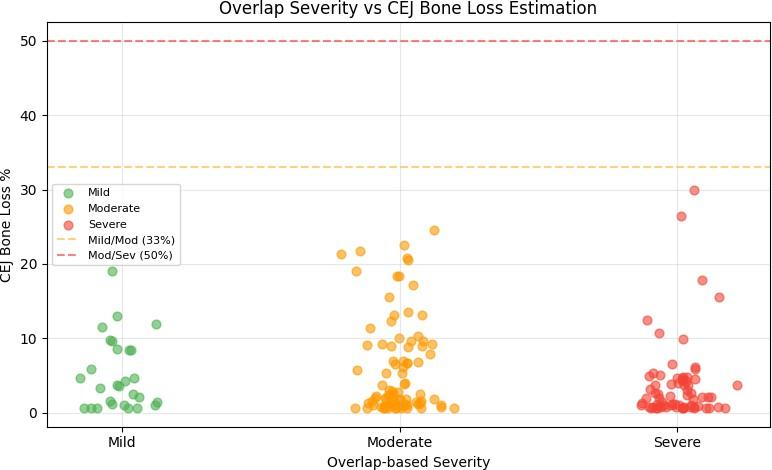
\includegraphics[width=0.62\textwidth]{figures/phase2/p2_6_04_cej_vs_overlap.jpg}
\caption[Phase 2 CEJ estimation against overlap severity]{Agreement of the CEJ heuristic with the
overlap-based severity labels (Phase 2 report, Figure 6.4).}
\label{fig:p2cejagree}
\end{figure}

\begin{table}[!htbp]
\centering
\caption[What Phase 3 found about the Phase 2 results]{What Phase 3 found about each Phase 2 result.}
\label{tab:p2corrections}
\small
\begin{tabularx}{\textwidth}{@{}L{3.6cm}Y@{}}
\toprule
Phase 2 result & Phase 3 finding\\
\midrule
Bone-loss binary, macro-F1 0.9233 & A crop-level split: every validation radiograph also supplied training crops. Held out by radiograph, the same model finds 3.4\% of labelled teeth (6 of 175); retrained by radiograph, 27.5\% at 95.9\% specificity (Section~\ref{sec:res-stage4})\\
``Bone loss'' label & The masks mark apical lesions, sclerosis and cysts; the output is reported as an abnormality flag\\
Bone-loss severity, macro-F1 0.7208 & Classes came from crop contrast; retrained on true overlap bands, 0.294 against 0.334 for a tooth-position prior: withheld\\
Caries severity, macro-F1 0.77 & Kept as Stage 3b; validated on the same 133 crops, not evaluated separately here\\
CEJ heuristic & Unchanged: a documented negative result\\
Integration ``not yet implemented'' & Six stages run end to end (Chapters~\ref{ch:system} and~\ref{ch:impl})\\
\bottomrule
\end{tabularx}
\end{table}
% {C040} {C041} {C042}

\section{Training Diagnostics}
\label{sec:res-train}

Every training loss in Figure~\ref{fig:training} falls steadily. Each kept checkpoint is the best on
its run's validation split, so these are selection diagnostics, not test results. % {C032}
\begin{itemize}
\item \textbf{Tooth detector.} Validation box mean average precision at IoU 0.5 (mAP@0.5) reaches
  0.634 at its last epoch and is still rising. On the frozen Tufts test split it missed its
  pre-registered guard, which required it to stay within four points of a Tufts-only control
  (0.587 against 0.723). It was adopted regardless, by a dated decision, for its numbering and caries
  behaviour.
\item \textbf{Lesion detector.} It peaks at mAP@0.5 0.820 (epoch 29 of 54).
\item \textbf{Numbering head.} Crop-level FDI-exact accuracy reaches 0.810 (epoch 12 of 15). The
  quadrant digit is right on 98.1\% of crops and the position digit on 82.5\%, so its errors are
  counting errors along the arch.
\item \textbf{Stage 4a.} Validation macro-F1 stays below 0.6 in all three seeds (best 0.568, 0.580
  and 0.597).
\end{itemize}
% {C031} {C032}

\begin{figure}[!htbp]
\centering
\includegraphics[width=\textwidth]{figures/repo/R04_training.pdf}
\caption[Training logs of the four trained stages]{Training logs of the four trained stages, from the
saved run files; validation splits, not test. (a) Tooth detector, 148 epochs, 150 Tufts radiographs.
(b) Lesion detector, 54 epochs, 1,200 CariesXrays radiographs. (c) Numbering head, 15 epochs, 6,450
tooth crops (DENTEX and Tufts, ground-truth boxes). (d) Stage-4a flag, three seeds of one recipe.
Dots: the checkpoint each run kept.}
\label{fig:training}
\end{figure}

On a published benchmark the detector family is competitive. Trained on CariesXrays alone, the lesion
detector's single-corpus arm reaches COCO AP 48.2 (AP50 84.5) on the project's seed-fixed 1,200-image
validation split. That matches the benchmark authors' task-specific method (48.2, AP50 84.1) and is six
points above the strongest of their ten baselines (42.2)~\cite{chen2024cariesxrays}. The splits
differ, and the project's split also chose the checkpoint, so the comparison is indicative only;
Section~\ref{sec:res-rq2} shows that this checkpoint does not transfer. The earlier detector lever is
summarised in Figure~\ref{fig:lever1}. % {C033}

\begin{figure}[!htbp]
\centering
\includegraphics[width=0.86\textwidth]{figures/repo/lever1_summary.png}
\caption[Lever 1, the first multi-corpus detector]{Lever 1, the first multi-corpus detector: numbering
on 164 DENTEX images rose (left), but the Tufts box-mAP guard failed (right), so it stayed an ablation.
Its successor, Lever A, is the shipped detector.}
\label{fig:lever1}
\end{figure}

\section{Identity: Detection and Numbering}
\label{sec:res-identity}

Table~\ref{tab:identity} measures the first two factors of the decision chain~\eqref{eq:chain}. On
DENTEX, whose other images trained the detector, identity costs 7.2 points. On the Tufts test split,
also from a training corpus, it costs 36.5. On UFBA-425, which no model trained on, it costs 55.5
points with the files as distributed. % {C030}

\begin{table}[!htbp]
\centering
\caption[Identity before disease]{Identity before disease: the first two factors of~\eqref{eq:chain},
per tooth, in percent. Det.: detected; Exact: numbered exactly, of those detected; End to end: their
product, with a 95\% cluster-bootstrap interval. DENTEX 164 images, Tufts test 143, UFBA-425 425 (as
distributed, and widened to a panoramic shape).}
\label{tab:identity}
\small
\begin{tabular}{@{}lrrrr@{}}
\toprule
Corpus & Teeth & Det. & Exact & End to end\\
\midrule
DENTEX & 936 & 99.6 & 93.2 & 92.8 [90.6, 94.9]\\
Tufts test & 3,760 & 89.3 & 71.1 & 63.5 [59.3, 67.5]\\
UFBA as is & 11,591 & 66.6 & 66.8 & 44.5 [42.4, 46.6]\\
UFBA widened & 11,591 & 95.6 & 80.8 & 77.2 [75.2, 79.1]\\
\bottomrule
\end{tabular}
\end{table}

End-to-end FDI-exact accuracy on DENTEX is 92.8\% (869 of 936 teeth) [90.6, 94.9], an in-domain
figure. Four teeth are not detected, and 93.2\% of the 932 found are numbered correctly. Of 63 wrong
codes, 51 (81.0\%) name an adjacent tooth in the correct quadrant (29 one step towards the midline, 22
one step away), and only 6 of 932 detected teeth (0.6\%) receive a quadrant-level error
(Figures~\ref{fig:numbering} and~\ref{fig:taxonomyerr}). Errors concentrate where adjacent teeth look
alike: 11.3\% of detected lateral incisors and 10.1\% of central incisors receive a wrong code,
against 4.1\% of second premolars. At molar positions, where most caries lies, 8.2\% of detected
second molars receive a wrong code, and each such error moves any finding to the wrong tooth. % {C034}

\begin{figure}[!htbp]
\centering
\includegraphics[width=\textwidth]{figures/repo/R08_numbering_reliability.pdf}
\caption[Outputs a constant cannot produce]{Outputs a constant cannot produce. (a) Numbering outcome
for each of 936 ground-truth DENTEX teeth (log scale). (b) Share of detected teeth given a wrong code,
by position. (c) Accuracy on the items answered as the least confident are declined: numbering, from
saved per-tooth confidences (circle: the 0.30 threshold fixed in code); crop classifier, saved
operating points at 50, 75, 90 and 100\% coverage. (d) Reliability of the crop classifier's raw
confidence on 863 held-out crops, by stated probability (marker area proportional to bin count).}
\label{fig:numbering}
\end{figure}

\begin{figure}[!htbp]
\centering
\includegraphics[width=0.94\textwidth]{figures/repo/stage2_failure_taxonomy_arm3c.png}
\caption[Numbering outcome taxonomy under the shipped detector]{Numbering outcome taxonomy under the
shipped detector, 936 DENTEX teeth: outcome categories (left) and the error rate by tooth position
(right).}
\label{fig:taxonomyerr}
\end{figure}

\section{The Positional Prior and the Image-Blind Constant}
\label{sec:res-constant}

On the fit set (Figure~\ref{fig:prior}) rule~\eqref{eq:rule} admits the eight first and second molars,
with prevalences from 0.372 (tooth 26) to 0.205 (tooth 27). It rejects the ninth code, tooth 15, at
0.128 against a threshold of 0.196, which is exactly the set the evaluation's greedy search returns.
Frozen, \{16, 17, 26, 27, 36, 37, 46, 47\} scores F1 0.392 on its fit images and 0.320 on the 164
scored ones: 286 true positives among 1,312 named codes, against 477 carious teeth, so its recall is
0.600, the share of carious teeth that lie on those eight molars. The prior shifts between the two
sets: teeth 17 and 27 fall to 0.140 and 0.134 on the scored images, so the oracle constant fitted on
the scored images themselves keeps six molars and reaches only 0.330. Almost all of the image-blind
score therefore needs no evaluation data. % {C010} {C011}

The set is fragile at its margin and the floor is not (Figure~\ref{fig:stability}). Refitted on 10,000
resamples of the fit images, rule~\eqref{eq:rule} returns exactly these eight molars 27\% of the time
and seven codes 45\% of the time, yet the refitted constants score a median F1 of 0.320 on the scored
images, 95\% of them between 0.279 and 0.330. Over sizes one to sixteen the constant's F1 is flat from
six to nine codes (0.298 to 0.325; Figure~\ref{fig:opcurve}). % {C012}

\begin{figure}[!htbp]
\centering
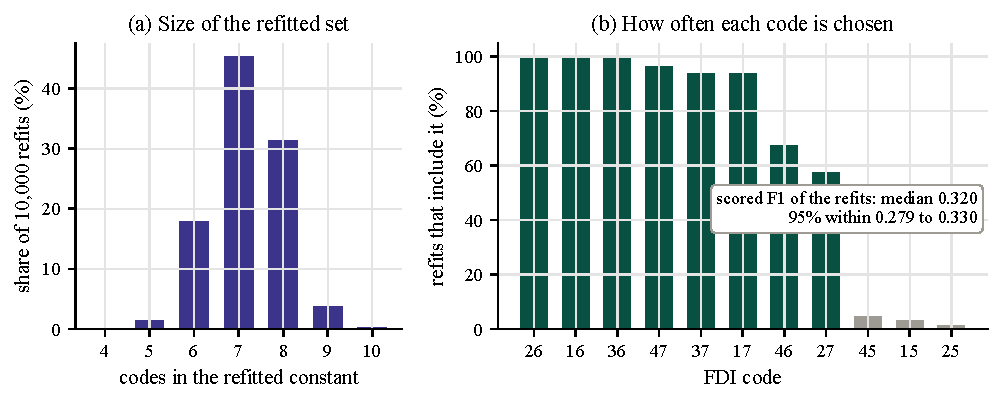
\includegraphics[width=\textwidth]{figures/plots/P2_constant_stability.pdf}
\caption[Stability of the fitted constant]{Stability of the fitted constant over 10,000 resamples of
the 78 fit images. (a) Size of the refitted set. (b) How often each code is chosen (teal: the eight
molars).}
\label{fig:stability}
\end{figure}

\begin{figure}[!htbp]
\centering
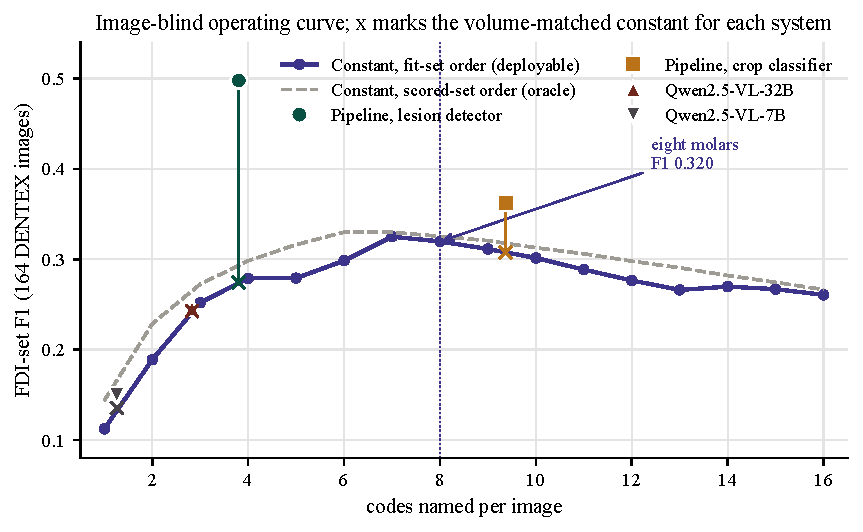
\includegraphics[width=0.94\textwidth]{figures/plots/P1_operating_curve.pdf}
\caption[Image-blind operating curve]{Image-blind operating curve: F1 of the $k$ most prevalent codes,
in fit-set order (deployable) and scored-set order (oracle), with each system at its own output volume.
A cross marks the image-blind answer that names as many codes as the system.}
\label{fig:opcurve}
\end{figure}

\section{RQ1 on Development Data}
\label{sec:res-rq1dev}

\begin{table}[!htbp]
\centering
\caption[Tooth-level caries prediction on DENTEX]{Tooth-level caries prediction on 164 DENTEX images
(477 carious teeth), micro-averaged. P: precision; R: recall; Matched: F1 minus that of a constant
naming as many codes (pp).}
\label{tab:ladder}
\small
\begin{tabular}{@{}lrrrr@{}}
\toprule
System & P & R & F1 & Matched\\
\midrule
Pipeline, lesion detector & 0.439 & 0.574 & 0.498 & +22.35\\
Pipeline, crop classifier & 0.237 & 0.765 & 0.362 & +5.50\\
Constant (image-blind) & 0.218 & 0.600 & 0.320 & ---\\
Qwen2.5-VL-32B, zero-shot & 0.250 & 0.243 & 0.246 & +0.39\\
Qwen2.5-VL-7B, zero-shot & 0.248 & 0.107 & 0.149 & +1.39\\
Oracle constant (test-fitted) & 0.245 & 0.505 & 0.330 & ---\\
\bottomrule
\end{tabular}
\end{table}
% {C013} {C014}

Both vision-language models see the radiograph and score below a list that does not
(Table~\ref{tab:ladder}): $-7.32$ points [$-11.23$, $-3.42$] for the 32B model and $-17.04$ [$-21.22$,
$-12.66$] for the 7B. The crop-classifier pipeline leads the constant by $+4.27$ points [$+1.58$,
$+7.05$] while naming 1,537 teeth to its 1,312, at barely higher precision (0.237 against 0.218), as
expected of a classifier that leans on the prior. The lesion-detector pipeline leads by $+17.80$
[$+13.48$, $+22.02$] and is the only system whose precision clearly exceeds the constant's: it names
624 codes, 43.9\% of them carious. % {C013} {C014}

Volume explains neither pipeline lead (Figure~\ref{fig:matched}). Against a matched constant that
names as many codes as the system, the leads are $+5.50$ [$+2.84$, $+8.22$] for the crop classifier and
$+22.35$ [$+17.42$, $+27.18$] for the lesion detector. The vision-language models are level with
constants of their own volume (32B [$-4.90$, $+5.63$], 7B [$-2.06$, $+4.85$]): they fall below the
eight molars by naming fewer teeth, and their F1 carries no detectable image information. % {C015}

\begin{figure}[!htbp]
\centering
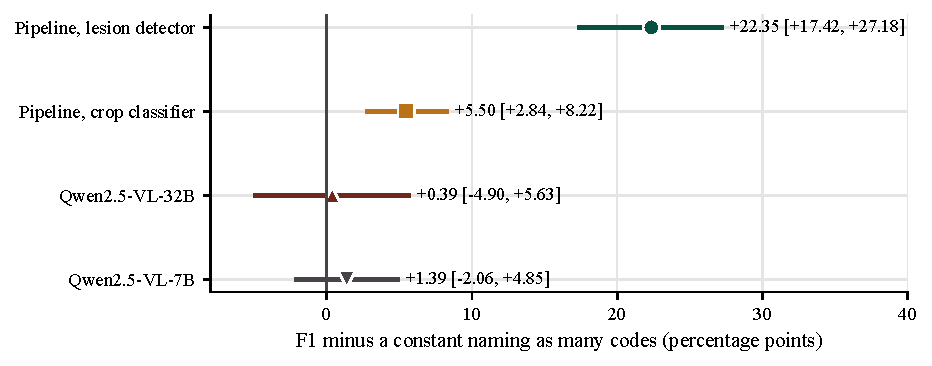
\includegraphics[width=0.86\textwidth]{figures/plots/P3_matched_volume.pdf}
\caption[Comparison at matched output volume]{Each system's F1 minus that of an image-blind answer
naming as many codes, with paired 95\% intervals over the 164 images.}
\label{fig:matched}
\end{figure}

Under lesion agreement the crop classifier leads the constant by $+17.12$ points [$+12.15$, $+21.89$],
partly by volume: it flags 1,439 teeth against 988, at a lower match rate (0.267 against 0.306). The
lesion detector flags 603 teeth at the highest match rate (0.473) and is not separable from the
constant ($-3.55$ [$-10.11$, $+2.64$]); F1 ranks it above the crop classifier, and agreement below.
None of this is yet evidence of perception, because the front end trained on this corpus. % {C025}

\section{RQ1 on External Data}
\label{sec:res-rq1ext}

On the four Ningxia sites the crop-classifier pipeline and the constant are level when pooled: 0.600
against 0.591, a difference of $+0.89$ points [$-3.86$, $+5.57$] (Figure~\ref{fig:paired}a). Per site,
the difference runs from $-18.99$ [$-26.32$, $-11.84$] at test1 to $+12.32$ [$+5.01$, $+19.20$] at test2
(Figure~\ref{fig:paired}b), a 31-point swing within one cohort. The constant's own agreement, each
site's prior mass on the eight molars, ranges from 0.494 to 0.709 (Figure~\ref{fig:sites}). On
CariesXrays the constant wins outright, 0.604 against 0.379 ($-22.42$ points [$-24.62$, $-20.18$]); it
flags 46\% more teeth but at the higher match rate (0.200 against 0.188), so volume does not explain it.
The crop-classifier pipeline leads only where its detector trained. % {C016}

\begin{figure}[!htbp]
\centering
\includegraphics[width=0.62\textwidth]{figures/repo/R07_paired_differences.pdf}
\caption[Lesion agreement of each caries option minus the constant]{Lesion agreement of each Stage-3a
option minus the constant, paired 95\% cluster-bootstrap intervals (10,000 resamples). (a) Per cohort;
DENTEX is development data for the front end and CariesXrays is the lesion detector's validation split.
(b) The four Ningxia sites, the pooled difference with sites fixed, and the DerSimonian--Laird mean for
the lesion detector (diamond; bar: 95\% interval; dotted, beyond the axis: prediction interval for a new
site).}
\label{fig:paired}
\end{figure}

\begin{figure}[!htbp]
\centering
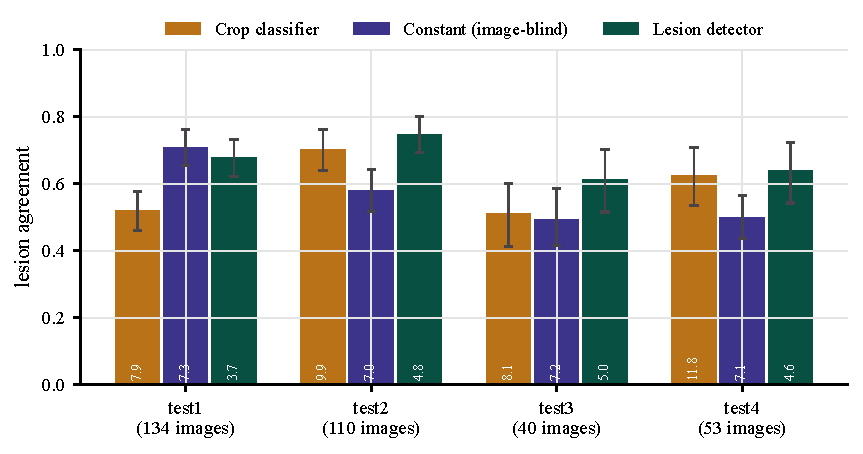
\includegraphics[width=0.92\textwidth]{figures/plots/P7_ningxia_sites.pdf}
\caption[Lesion agreement at each Ningxia site]{Lesion agreement at each Ningxia site for the three
Stage-3a options, with 95\% intervals. The numbers inside the bars are teeth flagged per image.}
\label{fig:sites}
\end{figure}

\section{RQ2: Localising Lesions Instead of Classifying Teeth}
\label{sec:res-rq2}

Five direct repairs of the crop classifier came first (Table~\ref{tab:repairs}), each against a same-day
control under a rule fixed in advance. None separated from zero, including a retrain with 2.67 times the
carious crops, so the ceiling is not set by supervision. Section~\ref{sec:res-shortcut} locates it in
the task as posed: a tight crop, a binary label and a strong prior. % {C017}

\begin{table}[!htbp]
\centering
\caption[Repairs of the crop classifier]{Repairs of the crop classifier on the same 863 held-out crops
(34 radiographs): paired difference in AP against the control (in F1 for the thresholds).}
\label{tab:repairs}
\small
\begin{tabular}{@{}lr@{}}
\toprule
Repair & Difference [95\% CI]\\
\midrule
Contrast equalisation (CLAHE) & $+0.049$ [$-0.003$, $+0.099$]\\
Crop expanded 1.25 times & $+0.020$ [$-0.037$, $+0.081$]\\
Position-balanced sampling & $+0.043$ [$-0.033$, $+0.116$]\\
Retrain, 2.67 times the positives & $-0.002$ [$-0.089$, $+0.082$]\\
Per-tooth-type thresholds (F1) & $+0.006$ [$-0.034$, $+0.041$]\\
\bottomrule
\end{tabular}
\end{table}

The task was then changed. Under the tooth detector of the time, the lesion detector met the
pre-registered rule on two cohorts of three: $+12.2$ points [$+10.1$, $+14.3$] over the constant on
CariesXrays and $+10.2$ [$+6.3$, $+14.0$] on Ningxia, with a tie on DENTEX ($-3.3$ [$-8.4$, $+1.3$]).
It was adopted on 4 September 2026. Table~\ref{tab:arms} gives the three options under the current
detector. % {C020} {C021}

\begin{table}[!htbp]
\centering
\caption[Lesion agreement of the three caries options]{Lesion agreement of the three Stage-3a options
under the current tooth detector: crop classifier (Clf.), constant (Const.) and lesion detector (Det.);
last column, detector minus constant in points, paired 95\% CI. CariesXrays is the detector's
validation split.}
\label{tab:arms}
\small
\begin{tabular}{@{}lrrrr@{}}
\toprule
Cohort & Clf. & Const. & Det. & Det.\ minus const.\\
\midrule
DENTEX & 0.802 & 0.630 & 0.595 & $-3.55$ [$-10.11$, $+2.64$]\\
CariesXrays & 0.379 & 0.604 & 0.757 & $+15.38$ [$+12.96$, $+17.73$]\\
Ningxia & 0.600 & 0.591 & 0.684 & $+9.28$ [$+4.72$, $+13.73$]\\
\bottomrule
\end{tabular}
\end{table}

Both consequences predicted in Section~\ref{sec:method-constant} hold.
\begin{itemize}
\item \textbf{Fewer flags.} The lesion detector flags 4.35 teeth per image against the constant's 7.15
  on Ningxia, and 2.16 against 7.05 on CariesXrays.
\item \textbf{More precise flags within each tooth type.} On DENTEX, the development corpus where
  per-type records exist, 46.3\% of the molars it flags carry caries, against 28.4\% for the crop
  classifier and 21.8\% for the constant; and 39.7\% of its flagged premolars against 17.0\%.
\end{itemize}
% {C023}
Per site (Figure~\ref{fig:pooling}) it is separated from the constant at test2, test3 and test4 ($+16.91$
[$+9.17$, $+24.62$], $+11.73$ [$+1.07$, $+21.34$], $+13.98$ [$+2.34$, $+24.34$]) and not at test1 ($-3.16$
[$-10.56$, $+3.97$]), where the constant is strongest. Treating the sites as a sample (random effects,
post hoc) gives $+9.61$ [$-0.54$, $+19.76$] (HKSJ [$-5.02$, $+24.24$]), $I^2 = 81\%$, $\tau$ 9.27 points
[3.22, 33.09] and a prediction interval of [$-36.08$, $+55.29$]. The lead therefore holds at three of
these four sites and is not shown for an unseen one. The training mixture, not the architecture,
transfers: the single-corpus arm reached 0.694 [0.674, 0.714] on CariesXrays but collapsed to 0.086
[0.055, 0.119] on DENTEX and 0.240 [0.209, 0.272] on Ningxia. % {C022} {C023} {C024}

\begin{figure}[!htbp]
\centering
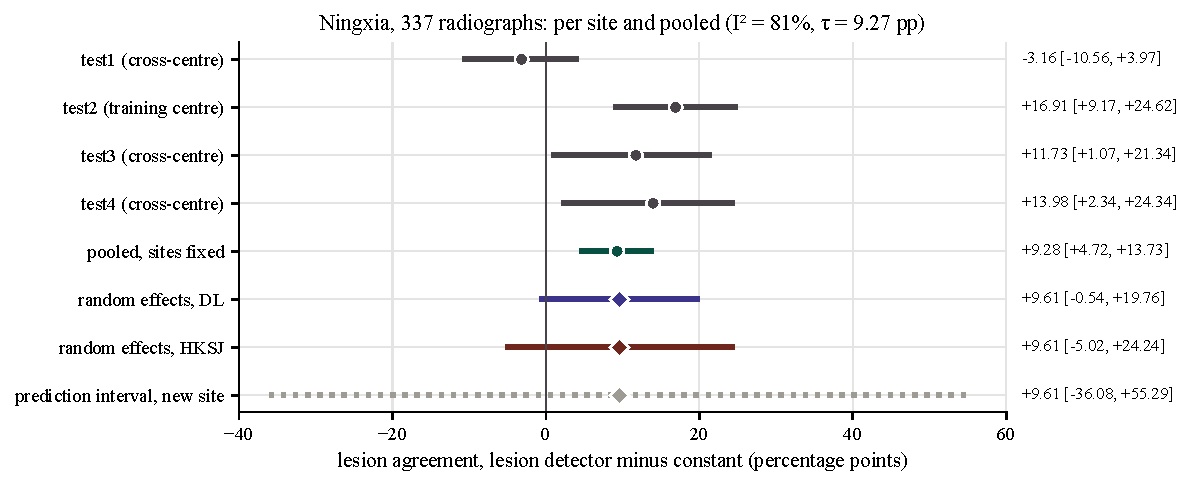
\includegraphics[width=0.94\textwidth]{figures/plots/P4_ningxia_pooling.pdf}
\caption[Ningxia: per site and pooled]{Lesion detector minus constant on Ningxia: each site, the pooled
difference with sites fixed, the random-effects mean with the DerSimonian--Laird and HKSJ intervals, and
the prediction interval for a new site.}
\label{fig:pooling}
\end{figure}

Figure~\ref{fig:outcomes} shows these numbers on images, in rows chosen by a rule fixed before
rendering: the scored image with the most lesions all found, a typical image, and the one with the most
lesions none found.

\begin{figure}[!htbp]
\centering
\includegraphics[width=0.86\textwidth]{figures/repo/R03_outcomes.pdf}
\caption[Pipeline output against the expert on three radiographs]{Pipeline output against the expert
on three held-out DENTEX radiographs: left, the lesion detector; right, the constant placed by the same
front end. (a) \texttt{test\_120}: all seven lesions found, 33 and 34 also flagged; the constant covers
four of the seven without reading the image. (b) \texttt{test\_0} (Figure~\ref{fig:walkthrough}): two
of three found, 48 missed. (c) \texttt{test\_110}: none of four found (32, 33, 34 and 46 missed; 16,
24, 26, 36 and 37 flagged). A flag without an annotated lesion is not a confirmed false positive: the
annotation's exhaustiveness is not documented. Radiographs: DENTEX~\cite{hamamci2023dentex},
CC~BY-NC-SA~4.0.}
\label{fig:outcomes}
\end{figure}

\section{The Positional-Shortcut Test}
\label{sec:res-shortcut}

\begin{table}[!htbp]
\centering
\caption[The positional-shortcut test on the crop classifier]{The positional-shortcut test on the crop
classifier: 863 held-out crops from 34 radiographs. Base rate: share carious in its training data.
Within-type AUC interval: cluster bootstrap over the 34 radiographs, 5,000 resamples.}
\label{tab:shortcut}
\small
\begin{tabular}{@{}lrrrrrr@{}}
\toprule
Tooth type & Crops & Carious & \makecell{Base\\rate} & \makecell{Mean score,\\healthy} & \makecell{Healthy\\flagged} & \makecell{Within-type\\AUC}\\
\midrule
Incisor & 266 & 8 & 0.017 & 0.075 & 0.039 & 0.681\\
Canine & 129 & 5 & 0.023 & 0.087 & 0.016 & 0.748\\
Premolar & 221 & 31 & 0.157 & 0.273 & 0.268 & 0.781\\
Molar & 247 & 83 & 0.343 & 0.478 & 0.482 & 0.781\\
All, within type & 863 & 127 & --- & --- & --- & 0.745 [0.660, 0.842]\\
\bottomrule
\end{tabular}
\end{table}

The classifier's mean score on healthy teeth climbs with the training base rate, from 0.075 on incisors
to 0.478 on molars, and it flags 48.2\% of healthy molars: the prior is doing visible work and costs
precision (Table~\ref{tab:shortcut}). Its within-type AUC is 0.745 [0.660, 0.842], above 0.5, so there
is also genuine lesion signal. A predictor that uses position alone and sees no image reaches
average precision (AP) 0.296, against the classifier's 0.550 and chance at 0.147. The classifier is
neither a lookup table nor a pure reader, but a reader whose score is inflated by a prior that the
constant captures for free. % {C018}

\section{RQ3: Outputs a Constant Cannot Produce}
\label{sec:res-rq3}

\textbf{Numbering} is covered in Section~\ref{sec:res-identity}.

\textbf{Selective prediction}~\cite{geifman2017selective} (Figures~\ref{fig:numbering}c
and~\ref{fig:coverage}). Declining the least-confident quarter raises numbering accuracy from 0.932 to
0.980 ($+4.76$ points [$+3.29$, $+6.54$], 164 image clusters) and the crop classifier's from 0.797 to
0.940 ($+14.25$ [$+11.32$, $+16.63$], 34 clusters). With confidences shuffled across items both gains
collapse, to $-0.06$ and $+0.00$ points, so the gain comes from the confidence ranking, not from
discarding items. The 0.30 threshold fixed in code lands at 96.1\% coverage and 0.941 accuracy. Because
coverage counts detected teeth, retaining 75\% of detections is 74.7\% of the teeth present. % {C035}

\begin{figure}[!htbp]
\centering
\includegraphics[width=0.94\textwidth]{figures/repo/c4_coverage_accuracy_arm3c.png}
\caption[Coverage against accuracy under abstention]{Coverage against accuracy as the least-confident
answers are declined: numbering (left, with the 0.30 threshold) and the crop classifier (right).}
\label{fig:coverage}
\end{figure}

\textbf{Calibration} (Figure~\ref{fig:calibration}) is measured on the crop classifier, because the
lesion detector emits detection scores rather than per-tooth probabilities. The classifier is
overconfident: at a stated confidence of 0.85 the observed share carious is 0.26, and its expected
calibration error (ECE)~\cite{naeini2015obtaining,guo2017calibration} is 0.136. Temperature scaling made
it worse (0.152). Isotonic regression reduced it to 0.043, at a cost: AP falls from 0.550 to 0.500, and
at the decision threshold 155 of 863 verdicts would change. Isotonic regression therefore adjusts only
the reported confidence. AP 0.550 [0.445, 0.660] against a prevalence of 0.147 shows a model that ranks
teeth well but fails at calibration and at its operating point. % {C036}

\begin{figure}[!htbp]
\centering
\begin{subfigure}[b]{\textwidth}
\centering
\includegraphics[width=0.86\textwidth]{figures/repo/caries_gate_calibration_test.png}
\caption{Reliability (raw) and precision--recall on the test crops.}
\end{subfigure}\\[2mm]
\begin{subfigure}[b]{0.46\textwidth}
\includegraphics[width=\textwidth]{figures/repo/caries_gate_temperature_scaling.png}
\caption{Temperature scaling ($T$ = 1.38).}
\end{subfigure}\hfill
\begin{subfigure}[b]{0.46\textwidth}
\includegraphics[width=\textwidth]{figures/repo/caries_gate_isotonic.png}
\caption{Isotonic calibration.}
\end{subfigure}
\caption[Calibration of the crop classifier]{Calibration of the crop classifier on 863 held-out test
crops.}
\label{fig:calibration}
\end{figure}

\section{The Abnormality Flag (Stage 4)}
\label{sec:res-stage4}

Stage 4's Phase 2 model reported 0.923 macro-F1 on a crop-level split in which every validation
radiograph also supplied training crops. That figure is a selected maximum, the best of 32 epochs on 59
positive crops. Held out properly, the model collapses (Table~\ref{tab:stage4},
Figure~\ref{fig:stage4}). % {C040}
\begin{itemize}
\item On 821 Tufts radiographs outside its training it found 7.6\% [5.19, 10.47] of the labelled teeth
  at 98.7\% specificity.
\item On the 125 test radiographs held out from its training it found 3.4\% (6 of 175).
\end{itemize}
% {C040}
Retrained with a radiograph-level split, three runs of one recipe found 27.5\%, 16.5\% and 11.0\% (50,
30 and 20 of 182) on 143 held-out radiographs, at 95.9\% to 98.6\% specificity. The seeds rank teeth
about equally well (AP 0.153 to 0.183); they differ in where the decision threshold falls. Seed 42 is
shipped. Against the previous model on the same teeth, its F1 for the labelled class is higher by
$+0.2135$ [$+0.1305$, $+0.2954$], and on the radiographs that carry a mask its AP exceeds a tooth-position
prior's (0.3504 against 0.2455; $+0.1049$ [$+0.0186$, $+0.2051$]). Both are the pre-registered
eligibility conditions. % {C040} {C041}

\begin{table}[!htbp]
\centering
\caption[Stage 4a: from the Phase 2 figure to the shipped model]{Stage 4a: from the Phase 2 figure to
the shipped model. Tufts data throughout.}
\label{tab:stage4}
\small
\begin{tabularx}{\textwidth}{@{}YL{3.0cm}rr@{}}
\toprule
Model and evaluation & Set & Sensitivity & Specificity\\
\midrule
Phase 2 model, crop-level validation & 1,558 crops & 0.8305 & 0.9953\\
Phase 2 model, held out & 821 radiographs & 0.076 & 0.987\\
Phase 2 model, test radiographs never trained on & 125 radiographs & 0.0343 & 0.9877\\
Radiograph split, seed 42 (shipped) & 143 radiographs & 0.2747 & 0.9590\\
Radiograph split, seed 43 & 143 radiographs & 0.1648 & 0.9806\\
Radiograph split, seed 44 & 143 radiographs & 0.1099 & 0.9863\\
\bottomrule
\end{tabularx}
\end{table}

\begin{figure}[!htbp]
\centering
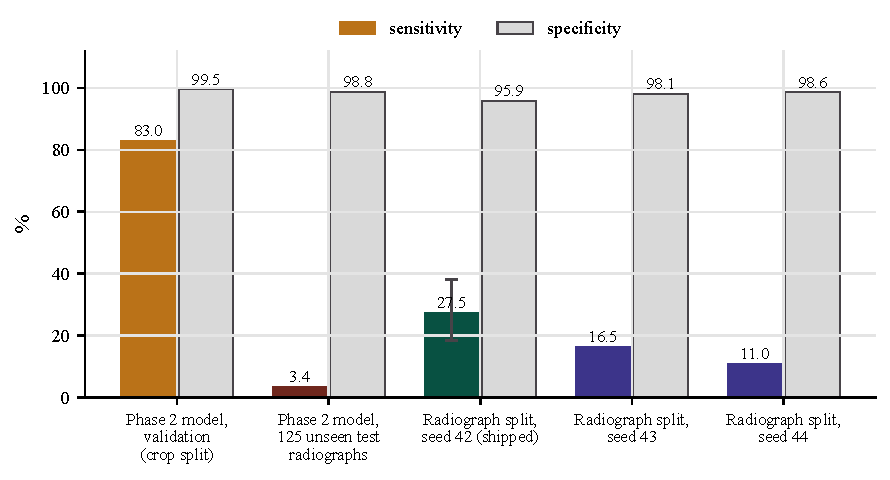
\includegraphics[width=0.94\textwidth]{figures/plots/P5_stage4_correction.pdf}
\caption[Stage 4a sensitivity and specificity]{Stage 4a sensitivity and specificity, from the Phase 2
validation figure to the radiograph-split retrain (error bar: 95\% interval of the shipped model).}
\label{fig:stage4}
\end{figure}

The severity head (macro-F1 0.294 [0.214, 0.385] against 0.334 for an image-blind position prior) stays
withheld, and no periodontal claim is made. The label itself is part of the explanation: the masks mark
apical lesions, sclerosis and cysts, so the collapse on external periodontitis annotations, where the
Phase 2 model found 2.4\% [2.0, 2.9] of the annotated teeth pooled over four Ningxia sites, is at least
partly a label mismatch rather than a failure to transfer. % {C042}

\section{Controls}
\label{sec:res-controls}

\textbf{Vision-language models without anatomy.} Shown no anatomy, the vision-language models return the
population prior. Qwen2.5-VL-7B answers ``26,~36'' to a blank grey image, to random noise and to a real
radiograph. Qwen2.5-VL-32B answers ``none'' to the blank image but answers noise with exactly the
constant's eight molars. One prompt was used and the decoding settings were not recorded, so this holds
for these models under this prompt. % {C019}

\textbf{Near-duplicate check.} A perceptual-hash search of the 164 scored DENTEX images against all 1,389
other DENTEX images found no further copy (Figure~\ref{fig:neardup}). As a positive control, all 86
MD5-identical images come out at distance 0 under both hashes, and all 86 were already excluded. No scored
image is at distance 0. The closest pHash pair is at 4 bits, with a dHash distance of 13. The 20
scored images with the nearest neighbours, inspected by eye, each differ from their neighbours in
restorations or missing teeth. The method finds copies of a radiograph, not a second radiograph of the
same patient. % {C060}

\begin{figure}[!htbp]
\centering
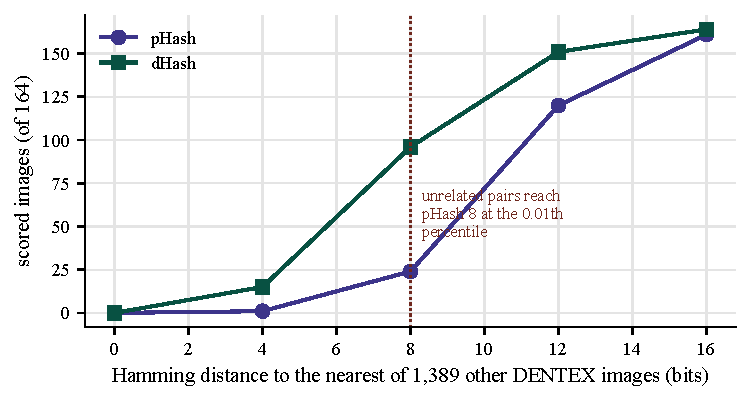
\includegraphics[width=0.78\textwidth]{figures/plots/P6_near_duplicates.pdf}
\caption[Near-duplicate check]{Scored DENTEX images whose nearest neighbour among the other DENTEX
images lies within a given Hamming distance, for pHash and dHash.}
\label{fig:neardup}
\end{figure}

\section{Runtime and Model Size}
\label{sec:res-runtime}

The whole pipeline runs at 1.70 seconds per image on the CPU of the team's macOS laptop, with no GPU
(1.45 seconds with the previous detector). The default configuration has 95.34\,M learnable parameters,
81.21\,M with the crop-classifier variant, and 72.99\,M for the caries path alone
(Figure~\ref{fig:params}). % {C001} {C003}

\begin{figure}[!htbp]
\centering
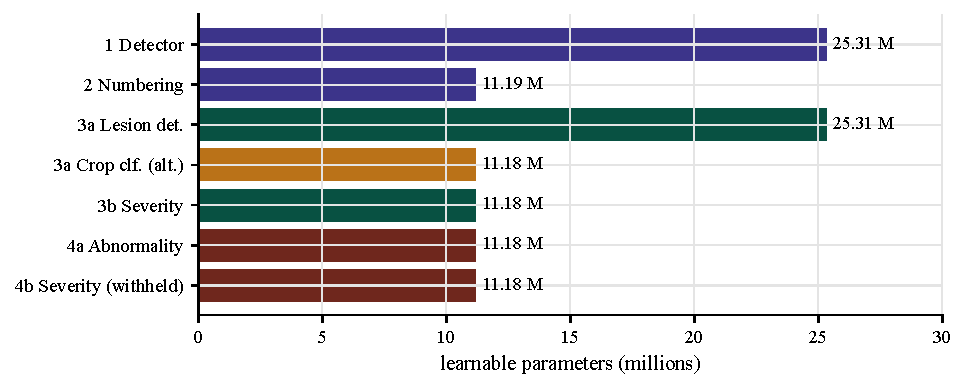
\includegraphics[width=0.86\textwidth]{figures/plots/P8_parameters.pdf}
\caption[Learnable parameters per stage]{Learnable parameters per stage, read from the saved weights
(batch-normalisation buffers excluded).}
\label{fig:params}
\end{figure}

\section{Discussion}
\label{sec:discussion}

The theory of Section~\ref{sec:method-constant} was formulated after the measurements, so
Table~\ref{tab:theory} is a consistency check, not a test of predictions made in advance. Five of its
implications hold, the last only at three of four sites; one of them is also expected under ordinary
domain shift and does not single out the theory. One is not supported: the prior inflates the
classifier's thresholded scores, but its ranking within a tooth type carries real image signal.

\begin{table}[!htbp]
\centering
\caption[What the theory implies, and what the measurements show]{What the theory implies, and what the
measurements show (a post-hoc consistency check).}
\label{tab:theory}
\small
\begin{tabularx}{\textwidth}{@{}L{4.2cm}YL{2.4cm}@{}}
\toprule
Implication & Evidence & Verdict\\
\midrule
Rule~\eqref{eq:rule} gives the best constant & reproduces the fitted eight molars; recall 0.600 equals the carious share at them & holds\\
The floor moves with the cohort & the constant's agreement is 0.494 to 0.709 across four sites & holds\\
A shortcut lifts healthy-tooth scores & healthy score 0.075 (incisors) to 0.478 (molars); 48.2\% of healthy molars flagged & holds\\
The shortcut carries the ranking & within-type AUC 0.745 [0.660, 0.842]; position-balanced AP $+0.043$ [$-0.033$, $+0.116$] & not supported\\
Development agreement does not transfer & classifier minus constant $+17.12$, $+0.89$ and $-22.42$ on the three cohorts & holds; not specific\\
Localising gives fewer, better flags & Ningxia $+9.28$ with 4.35 against 7.15 flags per image; DENTEX molar flags 46.3\% against 28.4\% carious & at 3 of 4 sites\\
\bottomrule
\end{tabularx}
\end{table}

\textbf{RQ1.} The same metric moves 40 points across cohorts and 31 across one cohort's sites, so a
favourable tooth-level figure on development data is weak evidence of perception.

\textbf{RQ2.} A detector that must place lesion boxes can express a positional prior only at a cost in
precision. It led the constant on the external sites with fewer flags, and on the development corpus its
flags were carious more often within each tooth type. Three facts qualify the lead:
\begin{itemize}
\item Ningxia informed the detector's adoption, so the lead measured there is optimistic.
\item The change of task is confounded with new training data.
\item The site-level interval includes zero; test1, where the constant is strongest, stays unexplained.
\end{itemize}

\textbf{RQ3.} Numbering, calibration and shuffle-controlled abstention are outputs a constant cannot
attempt, and they show confidence that ranks the system's own errors.

\textbf{What to report.} A tooth-level caries score should travel with an image-blind row fitted off the
test set, the identity factors of Table~\ref{tab:identity}, per-site external results with paired
intervals, and images of what the system does (Figures~\ref{fig:walkthrough}, \ref{fig:training}
and~\ref{fig:outcomes}). This complements the reporting checklists for medical-imaging and dental
AI~\cite{mongan2020claim,schwendicke2021checklist}. % {C090}

\section{Limitations}
\label{sec:limitations}

The authors' own limitations come first:
\begin{itemize}
\item DENTEX is in-domain for the tooth detector, which missed its Tufts guard (0.587 against 0.723).
  Only Ningxia is external to the lesion detector, it informed the adoption, and the random-effects
  interval includes zero. % {L001}
\item The theory treats codes independently and was checked on one corpus (78 and 164 images); the
  shortcut test rests on 34 radiographs; the lesion detector has no calibration curve. % {L002}
\item DENTEX caries labels were read from panoramic radiographs alone, which detect proximal caries less
  accurately than bitewings~\cite{akarslan2008comparison}. The expert lesions are therefore a subset of
  disease, and part of the molar prior may be a prior of what panoramic labels capture. % {L003}
\item Agreement has no negative class and the external cohorts have no healthy controls. Every model but
  Stage 4a is a single run, no clinician comparison was made, and the duplicate checks cannot find a
  patient's second radiograph. % {L004}
\item The Stage-4 label marks expert abnormalities, not periodontal bone loss; Stage 3b was validated
  only on 133 development crops. % {L005}
\end{itemize}

Additional caveats:
\begin{itemize}
\item The per-tooth-type comparison of flag precision was computed on DENTEX only. The saved Ningxia
  outputs hold per-image counts, so repeating it externally needs a re-run on the raw images.
\item The vision-language comparison used one prompt without recorded decoding settings.
\end{itemize}

\chapter{Conclusion and Future Work}
\label{ch:conclusion}

\section{Summary of the Work}

Phase 3 turned the separately trained modules of Phase 2 into one working system and then tested what
its output can and cannot show. A single OPG now passes through six stages and comes out as a numbered,
per-tooth JSON report with an overlay:
\begin{itemize}
\item YOLOv11l tooth detection;
\item ResNet18 numbering with one-to-one Hungarian assignment;
\item whole-image caries lesion detection;
\item caries severity grading;
\item an abnormality flag;
\item fusion with an assessability rule.
\end{itemize}
The system runs in 1.70 seconds per image on a laptop CPU, from the command line, in a Streamlit demo or
inside a Docker container, and every report records the checkpoints that produced it and their measured
limitations.

The evaluation showed why a tooth-level caries score must be read with care. Caries concentrates on the
first and second molars, so a fixed list of eight molars, the same for every patient and derived in
closed form, scores F1 0.320 on the held-out DENTEX images without reading a pixel. Against that floor
the shipped pipeline scores 0.498. Its lead is not bought by naming more teeth: an image-blind answer of
the same volume is 22.35 points lower. On 337 external radiographs from four sites the lesion detector
led the constant by 9.28 points of lesion agreement while flagging fewer teeth, at three of the four
sites. The earlier per-crop caries classifier, by contrast, was level with the constant externally, and
its scores on healthy teeth tracked each position's base rate. Phase 3 also corrected Phase 2: its
bone-loss figure of 0.9233 came from a crop-level split, and the radiograph-split retrain finds 27.5\%
of labelled teeth at 95.9\% specificity. % {C010} {C011} {C013} {C015} {C016} {C018} {C022} {C023} {C024} {C040}

\section{Utility}

\begin{itemize}
\item \textbf{For dentists and students,} the overlay and the per-tooth table give a second, numbered
  reading of an OPG, with each finding drawn on the tooth it refers to and the system's own uncertainty
  shown (doubtful codes, teeth that are not assessable). It is a teaching and research aid, not a
  diagnosis.
\item \textbf{For researchers,} the evaluation protocol is reusable:
  \begin{itemize}
  \item an image-blind row fitted off the test set;
  \item identity factors reported separately from disease;
  \item paired cluster-bootstrap intervals, reported per site;
  \item a matched-volume comparison;
  \item pre-registered adoption rules.
  \end{itemize}
\item \textbf{For maintainers,} hash-pinned checkpoints, a verified results trail and a self-testing
  container make every number in this report reproducible.
\end{itemize}

\section{Key Contributions}

\begin{enumerate}[label=\arabic*.,leftmargin=1.6em]
\item A complete, CPU-only, six-stage OPG-to-report pipeline, packaged for demonstration.
\item A closed-form image-blind floor for tooth-level caries scores, with its selection rule and a
  stability analysis.
\item A pre-registered change of the caries task from crop classification to lesion localisation, which
  led the floor externally with fewer flags.
\item Outputs a fixed list cannot produce: numbering with an error taxonomy, calibrated confidence and
  shuffle-controlled abstention.
\item An honest correction of the Phase 2 periodontal results.
\end{enumerate}

\section{Limitations}

The limitations are listed in Section~\ref{sec:limitations}:
\begin{itemize}
\item the external caries evidence rests on one cohort that informed the adoption;
\item DENTEX is in-domain for the detector;
\item the Stage-4 label is not periodontal bone loss;
\item there is no clinician comparison.
\end{itemize}

\section{Future Work}

\begin{enumerate}[label=\arabic*.,leftmargin=1.6em]
\item \textbf{External per-type precision.} Repeat the per-tooth-type comparison of flag precision on
  the raw Ningxia images, which needs a frozen-pipeline re-run that records per-tooth codes.
\item \textbf{Stronger shortcut controls.} Add a learned position-only floor, a content ablation, and a
  probe of whether the model can identify the site.
\item \textbf{Calibration of the lesion detector.} Fit and validate a calibrator for its detection
  scores, so that the default caries path also reports calibrated confidence and supports abstention.
\item \textbf{Explanations.} Add saliency maps (for example Grad-CAM) to the overlay, as planned in
  Phase 2.
\item \textbf{A real periodontal measurement.} Replace the abnormality proxy with bone-level labels:
  a learned CEJ and bone-crest landmark detector, on higher-resolution periapical or bitewing images
  where available.
\item \textbf{Numbering along the arch.} Reduce the off-by-one errors that remain, which the structural
  post-pass did not.
\item \textbf{Clinical evaluation.} Compare the system with dentists on a cohort with healthy controls
  and an independent reference standard such as bitewings.
\item \textbf{Release and publication.} Prepare a code and data availability statement, and submit the
  accompanying paper to a venue that meets the department's guidelines.
\end{enumerate}
% {C098}

The task hierarchy drawn in Phase 2 (Figure~\ref{fig:taskhier}) still describes the sequence of the
problem. Phase 3 built tooth detection, FDI numbering, disease detection, caries severity and the
clinical report into one working system, with input checks for image quality. Quantitative
bone-level measurement and explainability are the boxes that remain.

\begin{figure}[!htbp]
\centering

\includegraphics[width=\textwidth]{figures/phase2/p2_7_01_task_hierarchy.jpg}
\caption[Task hierarchy for panoramic radiograph analysis]{Task hierarchy for panoramic dental
radiograph analysis, adapted from the project's companion survey (Phase 2 report, Figure 7.1).}
\label{fig:taskhier}
\end{figure}


% ================================================================ references and appendices
\clearpage
\phantomsection
\addcontentsline{toc}{chapter}{REFERENCES}
\renewcommand{\bibname}{REFERENCES}
\begingroup
\titleformat{\chapter}[display]{\centering\bfseries\fontsize{18}{22}\selectfont}{}{0pt}{\MakeUppercase}
\singlespacing\small
\bibliographystyle{IEEEtran}
\bibliography{IEEEabrv,references}
\endgroup

\appendix
\renewcommand{\chaptertitlename}{Appendix}
\chapter{Definitions, Acronyms and Abbreviations}
\label{app:acronyms}

\section{Definitions}

The terms used in this report are defined in Table~\ref{tab:defs}.

\begin{table}[!htbp]
\centering
\caption[Definitions of terms used in the report]{Definitions of terms used in the report.}
\label{tab:defs}
\small
\begin{tabularx}{\textwidth}{@{}L{4.0cm}Y@{}}
\toprule
Term & Meaning in this report\\
\midrule
Assessable & A tooth record with an FDI code whose numbering confidence is at least 0.30\\
Constant (image-blind) & A fixed set of FDI codes answered for every image, without reading it; here the eight first and second molars\\
Fit set & The 78 DENTEX images, excluded from scoring because the models trained on them, on which the constant is fitted\\
Scored set & The 164 held-out DENTEX images on which the systems are compared\\
FDI-set F1 & Micro-averaged F1 over the set of tooth codes a system marks carious, per image\\
Lesion agreement & The share of expert lesions whose containing tooth is flagged by a system\\
Prior mass & The share of a cohort's lesions that lie on the constant's teeth\\
Matched-volume constant & An image-blind answer that names as many codes per image as a given system\\
Identity factors & Detection recall and numbering accuracy, the first two factors of the decision chain\\
Paired cluster bootstrap & Resampling radiographs (not teeth) with replacement, both systems on the same draw\\
Pre-registration & An acceptance rule committed to version control before the experiment it judges\\
Lever & A numbered, pre-registered proposal to change a pipeline component\\
Guard & A condition of a lever that must not get worse, such as Tufts detection accuracy\\
Abnormality flag & Stage 4a's output: the tooth crop overlaps an expert-marked Tufts abnormality\\
\bottomrule
\end{tabularx}
\end{table}

\section{Acronyms and Abbreviations}

The acronyms and abbreviations are expanded in Table~\ref{tab:acronyms}.

\begin{table}[!htbp]
\centering
\caption[Acronyms and abbreviations]{Acronyms and abbreviations.}
\label{tab:acronyms}
\small
\begin{tabularx}{\textwidth}{@{}L{2.2cm}YL{2.2cm}Y@{}}
\toprule
Acronym & Meaning & Acronym & Meaning\\
\midrule
AI & Artificial intelligence & JSON & JavaScript Object Notation\\
AP & Average precision & LLD & Low-level design\\
AP50 & Average precision at IoU 0.5 & mAP & Mean average precision\\
AUC & Area under the (ROC) curve & MD5 & Message-Digest 5 hash\\
CEJ & Cemento-enamel junction & NMS & Non-maximum suppression\\
CLAHE & Contrast-limited adaptive histogram equalisation & OPG & Orthopantomogram (panoramic radiograph)\\
CLI & Command-line interface & pHash, dHash & Perceptual and difference hashes\\
CNN & Convolutional neural network & PRS & Project requirements specification\\
CPU & Central processing unit & PRISMA & Preferred Reporting Items for Systematic Reviews and Meta-Analyses\\
DFD & Data-flow diagram & QUADAS-2 & Quality Assessment of Diagnostic Accuracy Studies, version 2\\
DL & DerSimonian--Laird (random effects) & ResNet & Residual network\\
ECE & Expected calibration error & ROC & Receiver operating characteristic\\
FDI & Fédération Dentaire Internationale (tooth notation) & RQ & Research question\\
FDP & Fixed dental prosthesis & SHA-256 & Secure Hash Algorithm, 256-bit\\
FPCL & Feature pyramid contrastive learning & UFBA-425 & The 425-radiograph dataset released with OralBBNet~\cite{budagam2024oralbbnet}\\
GPU & Graphics processing unit & VLM & Vision-language model\\
HKSJ & Hartung--Knapp--Sidik--Jonkman (interval) & YOLO & You Only Look Once (detector family)\\
HLD & High-level design & & \\
IoU & Intersection over union & & \\
\bottomrule
\end{tabularx}
\end{table}

\chapter{User Manual}
\label{app:manual}

\section{What the System Does}

The system takes one panoramic dental radiograph (OPG) and returns a per-tooth report: the FDI number
of every detected tooth, whether it shows caries and how deep, whether it overlaps an expert-style
abnormality, and whether the record is reliable enough to read. It is a research and teaching
prototype, \textbf{not a medical device}. Every report states that it is not clinically validated, and
its findings must not be used for diagnosis.

\section{Installation}

\begin{enumerate}[label=\arabic*.,leftmargin=1.6em]
\item Install Python 3.12 and Git.
\item Clone the repository; the default model checkpoints (313 MB) come with it.
\item Create a virtual environment and install the pinned packages:
\begin{lstlisting}
python -m venv .venv
.venv\Scripts\activate            (Windows)   or   source .venv/bin/activate
pip install -r requirements-lock.txt
\end{lstlisting}
\item Check the installation by running the tests (about one minute on a laptop):
\begin{lstlisting}
python -m pytest -q
\end{lstlisting}
\end{enumerate}

\section{Command-Line Use}

One image in, one report out:
\begin{lstlisting}
python scripts/run_inference.py --image opg.png --output report.json
python scripts/run_inference.py --image opg.png --output report.json --overlay overlay.jpg
\end{lstlisting}

\begin{table}[!htbp]
\centering
\caption[Command-line options]{Command-line options of \texttt{scripts/run\_inference.py}.}
\label{tab:cli}
\small
\begin{tabularx}{\textwidth}{@{}L{4.6cm}L{3.2cm}Y@{}}
\toprule
Option & Default & Effect\\
\midrule
\texttt{-{}-image} & (required) & the OPG to analyse (PNG or JPEG)\\
\texttt{-{}-output} & \texttt{report.json} & where to write the JSON report\\
\texttt{-{}-overlay} & none & also write an annotated image\\
\texttt{-{}-caries-method} & \texttt{lesion-detector} & \texttt{gate} selects the retained per-crop classifier\\
\texttt{-{}-caries-lesion-conf} & 0.25 & lesion detector confidence threshold (frozen; change only to experiment)\\
\texttt{-{}-assignment} & \texttt{hungarian} & optional structural numbering post-pass (an ablation)\\
\texttt{-{}-no-one-to-one} & off & plain argmax numbering, which can emit duplicate codes\\
\texttt{-{}-bone-severity-grade} & off & report the withheld Stage-4 severity grade\\
\texttt{-{}-detector}, \texttt{-{}-fdi-head} & shipped defaults & select another detector or numbering checkpoint\\
\texttt{-{}-caries-lesion-model}, \texttt{-{}-caries-gate}, \texttt{-{}-caries-severity} & shipped defaults & select other caries checkpoints\\
\texttt{-{}-bone-loss}, \texttt{-{}-bone-severity} & shipped defaults & select other Stage-4 checkpoints\\
\texttt{-{}-conf}, \texttt{-{}-det-iou}, \texttt{-{}-imgsz} & 0.25, 0.50, 1024 & detector settings (keep the defaults)\\
\bottomrule
\end{tabularx}
\end{table}

\section{Reading the Report}

\begin{itemize}
\item \textbf{\texttt{summary}} counts the detected and assessable teeth, the distinct and duplicate FDI
  codes (duplicates should be 0) and the positive findings.
\item \textbf{\texttt{teeth}} has one record per detected tooth, sorted by FDI code
  (Listing~\ref{lst:record}). Read a finding only if \texttt{assessable} is true; otherwise
  \texttt{not\_assessable\_reasons} says why.
\item \textbf{\texttt{caries.finding}} is \texttt{no\_caries}, \texttt{caries} or \texttt{deep\_caries}.
  With the default method its confidence is a detection score, not a calibrated probability.
\item \textbf{\texttt{bone\_loss.finding}} is \texttt{normal} or \texttt{bone\_loss}. It means that the
  tooth crop overlaps an expert-style abnormality, \emph{not} a periodontal bone-loss measurement.
\item \textbf{\texttt{limitations}} gives the measured accuracy of the checkpoints that ran and where it
  holds. Read it before trusting any number above it.
\item \textbf{Overlay colours.} Orange: a finding; blue: no finding; grey: not assessable. A thin line
  marks a numbering doubt.
\end{itemize}

\section{Web Demo}

\begin{enumerate}[label=\arabic*.,leftmargin=1.6em]
\item Start the demo from the repository root:
\begin{lstlisting}
python -m streamlit run app.py
\end{lstlisting}
\item Open \texttt{http://localhost:8501} in a browser. The first run loads the models, which takes a
  few seconds; later runs reuse them.
\item Upload an OPG (PNG or JPEG). The page shows the counts, the annotated overlay, the per-tooth table
  and the limitations (Figure~\ref{fig:app}).
\item Use \emph{Download full JSON report} to save the report, and \emph{Model versions used} to see
  which checkpoints ran.
\end{enumerate}
The demo is single-user, runs locally and stores nothing: the overlay is drawn in memory.

\begin{figure}[!htbp]
\centering
\begin{subfigure}[b]{0.49\textwidth}
\optionalgraphics[width=\textwidth]{figures/screens/app_01_landing.jpg}
\caption{Start page, waiting for an image.}
\end{subfigure}\hfill
\begin{subfigure}[b]{0.49\textwidth}
\optionalgraphics[width=\textwidth]{figures/screens/app_02_results.jpg}
\caption{Counts, overlay and per-tooth table.}
\end{subfigure}\\[3mm]
\begin{subfigure}[b]{0.72\textwidth}
\optionalgraphics[width=\textwidth]{figures/screens/app_03_limitations.jpg}
\caption{Limitations, the not-validated notice, the JSON download and the model versions.}
\end{subfigure}
\caption[The web demo]{The Streamlit web demo, captured on 6 November 2026 with DENTEX
\texttt{test\_0} (the radiograph of Figure~\ref{fig:walkthrough}). Its counts (30 teeth detected, 28
assessable, 4 caries-positive, no Stage-4 flag) match the saved report. Tooth 24 is not assessable
because its numbering confidence is 0.262. Radiograph: DENTEX~\cite{hamamci2023dentex},
CC~BY-NC-SA~4.0.}
\label{fig:app}
\end{figure}

\section{Docker}

\begin{lstlisting}
docker build -t opg-pipeline .
docker run -p 8501:8501 opg-pipeline
\end{lstlisting}
Then open \texttt{http://localhost:8501}. The build fails if a dependency would break the pipeline (a
CUDA build of PyTorch, NumPy 2 or an old Streamlit). The container's health is checked every 30 seconds.

\section{Reproducing a Reported Number}

\begin{lstlisting}
python scripts/verify_paper_numbers.py        # asserts 215 numbers against saved artefacts
python scripts/eval/verify_invariants.py      # twelve invariants of the saved outputs
\end{lstlisting}
Each evaluation script under \texttt{scripts/eval/} names its inputs and writes its result under
\texttt{outputs/}. The checkpoint behind any older number can be selected with the options in
Table~\ref{tab:cli}.

\section{Troubleshooting}

Common problems and their fixes are listed in Table~\ref{tab:trouble}.

\begin{table}[!htbp]
\centering
\caption[Troubleshooting]{Common problems and their fixes.}
\label{tab:trouble}
\small
\begin{tabularx}{\textwidth}{@{}L{5.2cm}Y@{}}
\toprule
Symptom & Fix\\
\midrule
\texttt{ImportError} from \texttt{scipy.optimize} & NumPy 2 is installed; install the pinned NumPy 1.26.4\\
``checkpoint not found'' & pull the repository again; the default checkpoints are versioned in it\\
The demo raises an error on upload & Streamlit is older than 1.62; install the pinned version\\
Report has input warnings & the image's bit depth or format is unusual; convert it to an 8-bit PNG\\
Many teeth not assessable & the image differs from the training corpora; read the limitations block\\
Duplicate FDI codes reported & \texttt{-{}-no-one-to-one} was given; remove it\\
\bottomrule
\end{tabularx}
\end{table}


\end{document}
